\documentclass[11pt,a4paper]{article}

\usepackage[a4paper,margin=1in]{geometry}
\usepackage[T1]{fontenc}
\usepackage[utf8]{inputenc}
\usepackage{lmodern}
\usepackage{microtype}
\usepackage{amsmath,amssymb,amsfonts,amsthm,mathtools}
\usepackage{bm}
\usepackage{booktabs}
\usepackage{array}
\usepackage{enumitem}
\usepackage{xcolor}
\usepackage[most]{tcolorbox}
\tcbuselibrary{skins,breakable}
\usepackage{hyperref}
\usepackage{framed}
\usepackage{titlesec}
\usepackage{fancyhdr}
\usepackage{lastpage}
\usepackage{tikz}
\usepackage{subcaption}
\usetikzlibrary{arrows.meta, positioning, calc, patterns, shapes.geometric}
\usepackage{graphicx}

\hypersetup{
    colorlinks=true,
    linkcolor=blue!60!black,
    urlcolor=blue!60!black,
    citecolor=blue!60!black,
    pdftitle={Computational Control -- Lecture Handout},
    pdfauthor={Riccardo Polo},
    pdfsubject={Dynamic Programming, LQR, MPC, Identification, Data-Driven Predictive Control, MDPs, Monte Carlo Learning, Reinforcement Learning}
}

\pagestyle{fancy}
\fancyhf{}
\fancyhead[L]{Computational Control}
\fancyhead[R]{Lecture Handout}
\fancyfoot[C]{\thepage\ / \pageref{LastPage}}

\titleformat{\section}{\large\bfseries}{\thesection}{0.6em}{}
\titleformat{\subsection}{\normalsize\bfseries}{\thesubsection}{0.6em}{}
\titleformat{\subsubsection}{\normalsize\itshape}{\thesubsubsection}{0.6em}{}

\setlist[itemize]{topsep=2pt,itemsep=2pt}
\setlist[enumerate]{topsep=2pt,itemsep=2pt}

\newcommand{\R}{\mathbb{R}}
\newcommand{\E}{\mathbb{E}}
\newcommand{\Prob}{\mathbb{P}}
\newcommand{\cS}{\mathcal{S}}
\newcommand{\cA}{\mathcal{A}}
\newcommand{\cU}{\mathcal{U}}
\newcommand{\cX}{\mathcal{X}}
\newcommand{\argmin}{\operatorname*{arg\,min}}
\newcommand{\tr}{\operatorname{tr}}
\newcommand{\norm}[1]{\left\lVert #1 \right\rVert}
\newcommand{\stagecost}{\ell}
\newcommand{\terminalcost}{V_f}

\newtheorem*{remark}{Remark}
\newtheorem*{idea}{Key idea}

% Colored theorem/statement box
\newtcolorbox{theorembox}[1][]{
    enhanced,
    breakable,
    colback=blue!5,
    colframe=blue!60!black,
    boxrule=0.7pt,
    arc=3pt,
    left=6pt,
    right=6pt,
    top=6pt,
    bottom=6pt,
    fonttitle=\bfseries,
    title=#1
}

\begin{document}

\begin{titlepage}
    \centering
    {\scshape\LARGE Computational Control\par}
    \vspace{0.6cm}
    {\huge\bfseries Lecture Handout\par}
    \vspace{0.8cm}
    \vfill
    {\large \today\par}
\end{titlepage}

\tableofcontents
\newpage

\section{Dynamic Programming and LQR}
\subsection{Introduction}
In general we formulate the optimization control task as
\begin{equation}
    \min_{\mathbf{u} \in \mathcal{U}} J(\mathbf{u})
    \label{eq:min1}
\end{equation}
where $\mathcal{U} = \mathcal{\tilde{U}}\times \{ 0,1,\dots,\text{T}\}$ is the set of the feasible inputs and $J(\mathbf{u}) $ is generally the sum of some \emph{stage costs} and a terminal cost/constraint.\\
The issue is that generally \ref{eq:min1} is an intractable optimization problem. This is due to several factors:
\begin{itemize}
    \item the dimension of $\mathbf{u}$ is too big;
    \item the cost function requires an accurate model of the system;
    \item the optimization problem is \textbf{non-convex};
    \item In presence of \textbf{disturbances} and \textbf{uncertainity} the open-loop nature of the task makes it useless
\end{itemize} 

In this context, Dynamic Programming (DP) is a powerfull tool whenever we can decompose the problem. In particular when the problem allows for a \textbf{Markovian representation}:
\begin{theorembox}[Key assumptions: Markovian representation]
The following hypothesis are crucial in order for DP to be meaningfull:
\begin{enumerate}
    \item There exists a \textbf{Markovian State}\footnote{i.e. $X_{t+1} \perp X_{1:t-1} | X_t$} that evolves according to some dynamics
    $$ x_{t+1} = f_t (x_t,u_t) \footnote{discrete time dynamical system representation. Notice $f_t$ can change with time}$$
    \item The initial condition $x_0$ is known.
    \item The cost is additive over time, i.e.
    $$J = \sum_{t} g_t (x_t,u_t)$$
\end{enumerate}
\end{theorembox}

In this context a powerfull result is given by \textbf{Bellman's principle}. Considering the following setup:
\begin{align*}
    \min_{\mathbf{u,x}} \quad &\sum_{t=0}^T g_t (x_t,u_t)\\
    \text{subject to} \quad &x_{t+1} = f_t(x_t,u_t)\\
                       &x_0 = X_0\\
                       &x_t \in \mathcal{X}_t \;\forall t\\
                       &u_t \in \mathcal{U}_t \; \forall t.
\end{align*}
a very powerfull result on which relies DP is \textbf{Bellman's optimality principle}.
\begin{theorembox}[Bellman's optimality principle]
\textit{An optimal policy has the property that whatever the initial state and the initial decisions are, the remaining decisions must consititute an optimal policy with regard to the state resulting from the first decision.}
\end{theorembox}
In a intuitive way we can say that any tail of an optimal trajectory is optimal too.\\
\begin{align*}
V_0(X_0)
&=
\min_{u_0}
\left\{
g_0(X_0,u_0 )
+
\min_{x_1,\dots,x_T \atop u_1,\dots,u_T}
\sum_{t=1}^{T} g_t(x_t,u_t)
\;\;
\text{s.t.}
\begin{cases}
x_{t+1} = f_t(x_t,u_t) \\
x_1 = f_0(X_0,u_0)
\end{cases}
\right\}
\\&= 
\min_{u_0}
\left\{
g_0(X_0,u_0)
+
V_1(x_1)
\right\}
\\&=
\min_{u_0}
\left\{
g_0(X_0,u_0)
+
V_1(f_0(x_0,u_0))
\right\}
\end{align*}
We can see that the problems are nested, therefore we need to proceed in a \textbf{backward} way, starting from the last time step and going backward in time. In particular we need to proceed in the following order
\begin{enumerate}
    \item solve the subproblem parametrized by $x_1$;
    \item compute the value function $V_1$;
    \item solve the outer problem 
    $$\min_{u_0} \{ g(X_0,u_0)+V_1(f_0(X_0,u_0)) \}$$
\end{enumerate}

\subsection{Dynamic Programming}
We can now write the general DP algorithm, which is a backward procedure to compute the value function and the optimal policy. We start from the last time step and we proceed backward in time until we reach the initial time step.\\
At the last stage (T) the subproblem is trivial, since there are no more decisions to be taken, therefore we have
$$V_T(x_T) = g_T(x_T)$$
At time $T-1$ we compute the value function as
\begin{align*}
    \min_{u_{T-1}} \{ g_{T-1}(x_{T-1},u_{T-1}) + V_T(f_{T-1}(x_{T-1},u_{T-1})) \}
\end{align*}
In particular notice that in the formulation above we know the value of $V_T(x_T)$, therefore we can compute the value function at time $T-1$ and so on until we reach the initial time step. So at this moment we have an optimal policy for the time step $T-1$, that means that we know how to compute the optimal control action at time $T-1$ given the state at time $T-1$. We can repeat this procedure until we reach the initial time step, therefore we have an optimal policy for all time steps.\\
At time $T-2$ we compute $V_{T-2}(x_{T-2})$ as
\begin{align*}
    \min_{u_{T-2}} \{ g_{T-2}(x_{T-2},u_{T-2}) + V_{T-1}(f_{T-2}(x_{T-2},u_{T-2})) \}
\end{align*}
Notice that this value function $V_{T-2}(x_{T-2})$ is a function of the state $x_{T-2}$, therefore we have to compute it $\forall x_{T-2} \in \mathcal{X}_{T-2}$, which is generally a very hard task.\\

\begin{theorembox}[Problem Decomposition]
We have seen that the optimal control problem is decomposed into \textbf{stage problems} that we can solve via \textbf{backward induction} :
\begin{align}
V_t(x_t) = \min_{u_t} \{ g_t(x_t,u_t) + V_{t+1}(f_t(x_t,u_t)) \}
\end{align}
And $V_T(x_T) = g_T(x_T)$
\end{theorembox}
A reasonable question at this point would be, in which cases is this stage problem formulation simple to solve ? We can list three scenarios:
\begin{itemize}
    \item Decision space $\mathcal{\tilde{U}}$ is convec , or maybe finite.
    \item If $g_t$ is convex in $u_t$.
    \item If $V_{t+1}$ evaluated at the future step $f_t$ is convex in $u_t$.
\end{itemize}
In practice, a very common setup in which the assumptions above are satisfied is when we have a \textbf{quadratic cost} $g_t$ and a \textbf{linear dynamics} $f_t$, which is the so called \textbf{LQR problem}. Another way is also to use approximations of the value function, in which case maybe not all the assumptions above are satisfied, but we can still solve the stage problem.

\subsection{Optimal LQR}
The LQR problem is a special case of the optimal control problem, in which we have a linear dynamics and a quadratic cost. In particular we have:
\begin{itemize}
    \item Markovian update and linear dynamics
    $$ x_{t+1} = A_t x_t + B_t u_t$$
    \item Quadratic cost function:
    $$ \sum_{t=0}^{T-1} \left( x_t^\top\, Q_t\, x_t + u_t^\top\, R_t\, u_t \right) + x_T^\top \,S \,x_T \quad \text{with }Q,S\geq 0 \, , \, R >0 $$
    \item Value function (i.e. minimum cost to go starting from $x$ at time $t$) :
    $$V_t (x) = \min_{u_t,\dots,u_{T-1}} \sum_{k=t}^{T-1} \left( x_k^\top\, Q_k\, x_k + u_k^\top\, R_k\, u_k \right) + x_T^\top \,S \,x_T$$
    \begin{align*}
        \text{subject to } &x_{k+1} = A_k x_k + B_k u_k \quad \forall k=t,\dots,T-1 \\
        &x_t = x
    \end{align*}
\end{itemize}
We say that the optimal cost is $V_0(x_0)$.

\subsection{Dynamic Programming for LQR}

Let us now specialize the dynamic programming recursion to the Linear Quadratic Regulator (LQR) problem.  
Recall that the value function represents the optimal \emph{cost-to-go}, i.e. the minimum cost achievable from a given state when acting optimally from that point onward.

A key observation in the LQR setting is that the terminal cost is quadratic in the state.  
Indeed, from the problem formulation we have
\[
V_T(x) = x^\top S x ,
\]
which is a convex quadratic function since $S \succeq 0$.

The main idea of the LQR derivation is to show that the value function $V_t(x)$ is also quadratic and has the form of $V_t(x) = x^\top\, P_t \,x$ for some symmetric positive semidefinite matrix $P_t$.\\
We will then show that the matrices $P_t$ can then be computed recursively by working \emph{backward in time} starting from the terminal time $T$.
Eventually the the optimal control input $u_t$ will be computed as a solution of a convex quadratic optimization problem, which admits a closed-form solution.\\

To derive the recursion, consider the dynamic programming stage problem at time $t$ where the value function is 
$$ 
V_t(x) = \min_{u} \Big( x^\top\, Q \,x + u^\top\, R \,u + V_{t+1}(A x + B u) \Big).
$$
We now proceed by induction, assuming that $V_{t+1}(x) = x^\top P_{t+1} x$ for some positive semidefinite matrix $P_{t+1}$. Then $V_t(x)$ can be written as
\begin{align*}
V_t(x) &= x^\top Q x + \min_{u} \Big(u^\top R u + (A x + B u)^\top P_{t+1} (A x + B u) \Big) \\
&= x^\top Q x + \min_{u} \Big(
\textcolor{blue}{u^\top R u}
+ x^\top A^\top P_{t+1} A x
+ 2 u^\top B^\top P_{t+1} A x
+ \textcolor{blue}{u^\top B^\top P_{t+1} B u}
\Big) \\
&= x^\top \, Q \, x  + \min_{u} \Big(
\textcolor{blue}{u^\top (R + B^\top P_{t+1} B) u} 
+ x^\top A^\top P_{t+1} A x
+ 2 u^\top B^\top P_{t+1} A x
\Big).
\end{align*}
We set the gradient of the expression inside the minimization with respect to $u$ to zero:
$$ (R+B^\top P_{t+1} B) u + B^\top P_{t+1} A x = 0 $$
Yielding the optimal control input
$$\boxed{\textcolor{red}{u^* = - (R + B^\top P_{t+1} B)^{-1} B^\top P_{t+1} A x}}$$
But now we need to check that $V_t(x)$ is indeed quadratic in $X$. That means $V_t(x) = x^\top P_t x$ for some $P_t$ and we have to find how to compute $P_t$. We can do that by plugging the optimal control input $u^*$ back into the expression for $V_t(x)$:
% remove green color in following code
\begin{align*}
V_t(x)
&= x^\top Q x + (u^*)^\top R u^* + (A x + B u^*)^\top P_{t+1} (A x + B u^*) \\[4pt]
&= x^\top Q x
+ \textcolor{blue}{(u^*)^\top R u^*}
+ x^\top A^\top P_{t+1} A x
+ 2 (u^*)^\top B^\top P_{t+1} A x
+ \textcolor{blue}{(u^*)^\top B^\top P_{t+1} B u^*} \\[6pt]
&= x^\top Q x
+ x^\top A^\top P_{t+1} A x
+ \textcolor{blue}{(u^*)^\top (R + B^\top P_{t+1} B) u^*}
+ 2 (u^*)^\top B^\top P_{t+1} A x \\[6pt]
&= x^\top Q x
+ x^\top A^\top P_{t+1} A x
+ \textcolor{red}{(u^*)^\top} \bigr( (R+B^\top P_{t+1} B)\textcolor{red}{u^*} + 2 B^\top P_{t+1} A x \bigl) \\[6pt]
&=x^\top Q x
+ x^\top A^\top P_{t+1} A x\\
&\textcolor{red}{- \bigl((R+B^\top P_{t+1} B)^{-1} B^\top P_{t+1} A x\bigr)^\top} \bigr( \textcolor{red}{-}(R+B^\top P_{t+1} B)\textcolor{red}{(R+B^\top P_{t+1} B)^{-1} B^\top P_{t+1} A x} + 2 B^\top P_{t+1} A x \bigl) \\[6pt]
&=x^\top Q x
+ x^\top A^\top P_{t+1} A x + 
- \bigl((R+B^\top P_{t+1} B)^{-1} B^\top P_{t+1} A x\bigr)^\top \bigl( B^\top P_{t+1} A x \bigr) \\[6pt]
&= x^\top Q x
+ x^\top A^\top P_{t+1} A x
- x^\top A^\top P_{t+1} B
(R + B^\top P_{t+1} B)^{-1}
B^\top P_{t+1} A x \\[6pt]
&=
x^\top
\Big(\textcolor{blue}{
Q + A^\top P_{t+1} A
-
A^\top P_{t+1} B
(R + B^\top P_{t+1} B)^{-1}
B^\top P_{t+1} A}
\Big)
x \\[6pt]
&= x^\top \textcolor{blue}{P_t} x
\end{align*}
To complete the proof one should check that $P_t$ is positive semidefinite. Here we homit the proof. $\quad  \blacksquare$\\
In cocnlusion we have been able to derive a closed-form expression for the optimal control input $u^*$ for the LQR problem.Be aware that this solution is not valid anymore if the problem becomes constrained.\\
 
We summerize here the main results:
\begin{theorembox}[Optimal LQR solution]
\textbf{Backward induction} 
$$u_t = \underbrace{- (R + B^\top P_{t+1} B)^{-1} B^\top P_{t+1} A}_{\Gamma_t} \,x_t$$
where
$$P_t = Q + A^\top P_{t+1} A - A^\top P_{t+1} B (R + B^\top P_{t+1} B)^{-1} B^\top P_{t+1} A \quad \text{and } P_T = S$$
\textbf{Forward integration from } $x_0$:
$$x_{t+1} = A x_t + B u_t$$
\end{theorembox}
So clearly one could compute this whole open-loop sequence $u_0,\dots,u_{T-1}$ in a offline computation. But what if the optimal control input $\mathbf{u}$ takes us to a trajectory different from the one we compouted ? In this case we can use the optimal policy $\Gamma_t$ to compute the optimal control input at each time step, given the current state $x_t$. This is the main advantage of having a closed-form solution for the optimal control input, since we can use it in a feedback way.\\

We can do a quick comparison of the computational cost of using these equations in a feedback way vs computing the whole open-loop sequence. By fixing $m$ as the size of the states and $n$ as the size of the control input, we have the following computational costs:
\begin{itemize}
    \item \textbf{Offline computation}
    \begin{itemize}
        \item $n\times n$ matrix multiplications to compute $P_t$ for $t=T-1,\dots,0$
        \item $m\times m$ matrix inversions to compute $\Gamma_t$ for $t=T-1,\dots,0$
        \item $T$ iterations to compute $P_t$ and $\Gamma_t$ for $t=T-1,\dots,0$
    \end{itemize}
    \item \textbf{Online computation}
    \begin{itemize}
        \item Storage of $T$ $m\times n$ matrices $\Gamma_t$ for $t=T-1,\dots,0$
        \item $m\times m$ matrix multiplications to compute $u_t$ at each time step, given $x_t$
    \end{itemize}
\end{itemize}

\subsubsection{Infinite-Horizon LQR}

In many practical control applications the system is required to operate
over a very long time horizon.  
Examples include regulation problems where the controller must stabilize
a system indefinitely, or tracking tasks where disturbances may occur
continuously.

For these reasons it is natural to study the limit case where the horizon
tends to infinity. The resulting problem is known as the
\textbf{infinite-horizon Linear Quadratic Regulator (LQR)}.

Consider the linear time-invariant system
\[
x_{t+1} = A x_t + B u_t, \qquad x_0 \text{ given}
\]

and the infinite-horizon quadratic cost
\[
\min_{u_0,u_1,\dots}
\sum_{t=0}^{\infty}
\left(
x_t^\top Q x_t + u_t^\top R u_t
\right),
\qquad Q \succeq 0, \; R \succ 0 .
\]

Compared to the finite-horizon case, the cost now accumulates
indefinitely. Therefore a first important question concerns the
\textbf{feasibility} of the problem.

\begin{theorembox}[Feasibility]
If the pair $(A,B)$ is \textbf{stabilizable}, then there exists a control input
sequence that yields a finite value of the infinite-horizon cost.
\end{theorembox}

Indeed, if the system is stabilizable there exists a feedback matrix
$K$ such that the closed-loop matrix $A + BK$ has all eigenvalues
inside the unit circle.  
Consider the linear feedback policy
\[
u_t = K x_t .
\]

The state then evolves according to
\[
x_t = (A + BK)^t x_0 .
\]

Substituting this into the cost yields
\[
V(x_0)
=
\sum_{t=0}^{\infty}
\left(
x_t^\top Q x_t
+
x_t^\top K^\top R K x_t
\right).
\]

Using the closed-loop dynamics we obtain
\[
V(x_0)
=
x_0^\top
\left(
\sum_{t=0}^{\infty}
(A+BK)^{t\top}
(Q + K^\top R K)
(A+BK)^t
\right)
x_0 .
\]

Since $A+BK$ is stable, the above summation behaves like a
\emph{matrix geometric series} and therefore converges.
Consequently the cost is finite.\\

But how do we compute the optimal policy for the infinite-horizon LQR problem ? The answer is that we can still apply the dynamic programming recursion, but now the value function does not depend on time. The solution is given by the \textbf{Discrete Algebraic Riccati Equation (DARE)}, which is a fixed-point equation for the matrix \(P\) that defines the value function.
\begin{theorembox}[Algebraic Riccati Equation]
The iteration 
$$P_{t-1} = Q + A^\top P_t A - A^\top P_t B (R + B^\top P_t B)^{-1} B^\top P_t A\qquad P_0 = 0$$
converges, for $t \to -\infty$, to a unique positive semidefinite solution \(P_{\infty} \succ 0\) of the algebraic Riccati equation
$$ \textcolor{red}{P} = Q + A^\top \textcolor{red}{P} A - A^\top \textcolor{red}{P} B (R + B^\top \textcolor{red}{P} B)^{-1} B^\top \textcolor{red}{P} A $$
\end{theorembox}
We can show that then the optimal feedback control in the infinite-horizon case is given by
$$u_t = \underbrace{- (R + B^\top P B)^{-1} B^\top P A}_{F_{\infty}} x_t  $$
and thus minimizes the infinite horizon cost and yields $V(X_0) = X_0^\top P X_0$.\\
We now show again a comparison of the computational cost of using the infinite-horizon solution in a feedback way vs computing the whole open-loop sequence. By fixing $m$ as the size of the states and $n$ as the size of the control input, we have the following computational costs:
\begin{itemize}
    \item \textbf{Offline computation}
    \begin{itemize}
        \item $n\times n$ matrix multiplications to compute $P$
        \item $m\times m$ matrix inversions to compute $F_{\infty}$
        \item $T$ iterations to compute $P$ and $F_{\infty}$ for $t=T-1,\dots,0$
        \item "Infinite iterations" to compute $P$ for $t \to -\infty$\footnote{$P_{\infty}$ can be computed by solving the Algebraic Riccati Equation}
    \end{itemize}
    \item \textbf{Online computation}
    \begin{itemize}
        \item Storage of a \textbf{single} $m\times n$ matrix $F_{\infty}$. So less memory is required compared to the finite-horizon case, since we do not need to store $T$ matrices $\Gamma_t$.
        \item $m\times n$ matrix multiplications to compute $u_t$ at each time step, given $x_t$
    \end{itemize}
\end{itemize}

A natural question at this point is whether the optimal infinite-horizon
feedback law is also \emph{stabilizing}.  
Indeed, even if the infinite-horizon cost is well defined and the Riccati
equation admits a solution, one would still like to know whether the
resulting closed-loop dynamics
\[
x_{t+1} = (A + B F_\infty)x_t
\]
are asymptotically stable.

This is a meaningful question because the quadratic cost does \emph{not}
necessarily penalize all state directions. In particular, if some unstable
state component is not ``seen'' by the cost, then the optimizer may have
no incentive to stabilize it.

\paragraph{Illustrative example}

Consider the system
\[
x_{t+1} =
\begin{bmatrix}
2 & 0\\
0 & 3
\end{bmatrix}x_t + u_t,
\qquad
Q =
\begin{bmatrix}
1 & 0\\
0 & 0
\end{bmatrix},
\qquad
R =
\begin{bmatrix}
1 & 0\\
0 & 1
\end{bmatrix}.
\]

Here both open-loop modes are unstable, since the eigenvalues of \(A\) are
\(2\) and \(3\). However, the stage cost penalizes only the first state
component \(x_1\), while the second component \(x_2\) does not appear in
the state cost. Therefore, from the viewpoint of the objective function,
an unstable behavior in the second state may go completely unnoticed
unless it is indirectly forced to be controlled through the dynamics.

This already suggests an important principle:

\begin{quote}
Unstable modes must be visible in the cost function, otherwise the optimal
controller may fail to stabilize them.
\end{quote}

To make this statement precise, write $Q = C^\top C$.
Then the cost penalizes exactly the directions that are observable through
the pair \((C,A)\).

\begin{theorembox}[Stability of the optimal infinite-horizon LQR controller]
Let \(Q = C^\top C\).  
The optimal infinite-horizon feedback \(F_\infty\) stabilizes the system
if and only if
\begin{enumerate}
    \item the pair \((A,B)\) is stabilizable;
    \item the pair \((C,A)\) has no unobservable unstable modes.
\end{enumerate}
Equivalently, all unstable modes of \(A\) must be detectable through the
state penalty \(Q\).
\end{theorembox}

The second condition is often stated by saying that the pair
\((A,Q^{1/2})\) must be \textbf{detectable}.  
Detectability is weaker than observability: it does not require all modes
to be observable, but only the unstable ones.

\paragraph{Interpretation}

This theorem has a clear practical meaning.  
The matrix \(R\) penalizes the control effort, while \(Q\) determines which
state directions the controller tries to regulate. If an unstable mode is
not penalized by \(Q\), then the optimization problem may prefer not to
spend control effort on that mode, since doing so does not improve the
objective. As a consequence, the optimal controller may exist but fail to
stabilize the closed-loop system.

Hence, in practice:

\begin{itemize}
    \item \((A,B)\) stabilizable ensures that unstable modes can in principle
    be controlled;
    \item detectability of \((A,Q^{1/2})\) ensures that every unstable mode
    matters in the cost.
\end{itemize}

When both conditions hold, the stabilizing solution \(P\) of the algebraic
Riccati equation yields the optimal feedback
\[
u_t = F_\infty x_t,
\qquad
F_\infty = - (R + B^\top P B)^{-1} B^\top P A,
\]
and the closed-loop matrix \(A + B F_\infty\) has all eigenvalues inside
the unit disk.

\newpage
\section{Model Predictive Control}
\subsection{Introduction}
In the previous chapter we have seen an overview of the LQR problem and how to solve it using dynamic programming. In that formulation, we assumed that there were no constraints on the state and control input. However, in many real-world applications, constraints on the state and input must be explicitly taken into account.\\
In the presence of constraints, the problem cannot, in general, be solved in closed form via backward induction as in the unconstrained LQR case, since the value function is no longer quadratic.The resulting optimization problem becomes:

\begin{theorembox}[Constrained LQ finite horizon problem]
\begin{align*}
\min_{u_0, \ldots, u_{T-1},x_0,\dots,x_T} &\sum_{t=0}^{T-1} \left( x_t^\top Q x_t + u_t^\top R u_t \right) + x_T^\top S x_T \\
\text{s.t.} \quad & x_{t+1} = A x_t + B u_t, \quad t=0, \ldots, T-1 \\
& x_0 = x_0 \\
& \textcolor{red}{x_t \in \mathcal{X}_t}\\
& \textcolor{red}{u_t \in \mathcal{U}_t}
\end{align*}
Usually, the constraint sets are convex, e.g., polytopes.
\end{theorembox}

One could solve this optimization problem in a \textbf{one-shot} fashion (i.e., open-loop strategy), obtaining an optimal input sequence $u_0, \ldots, u_{T-1}$ for the given initial state $x_0$, instead of a state-feedback policy as in the unconstrained case (where $u_t = \Gamma_t x_t$).\\ However, if disturbances or model mismatch cause the system to deviate from the predicted trajectory, the previously computed control sequence is no longer optimal. As a result, the system will follow a different trajectory than expected (see Figures \ref{fig:mpc_01} and \ref{fig:mpc_02}).\\
To address this issue, the optimal control problem must be re-solved using the updated state information. Since we assume a Markovian system, the current state contains all the information needed to compute an optimal control sequence for the future. This implies that the optimization problem must be solved repeatedly, at each time step, within one sampling interval.

\begin{figure}[!ht]
\centering
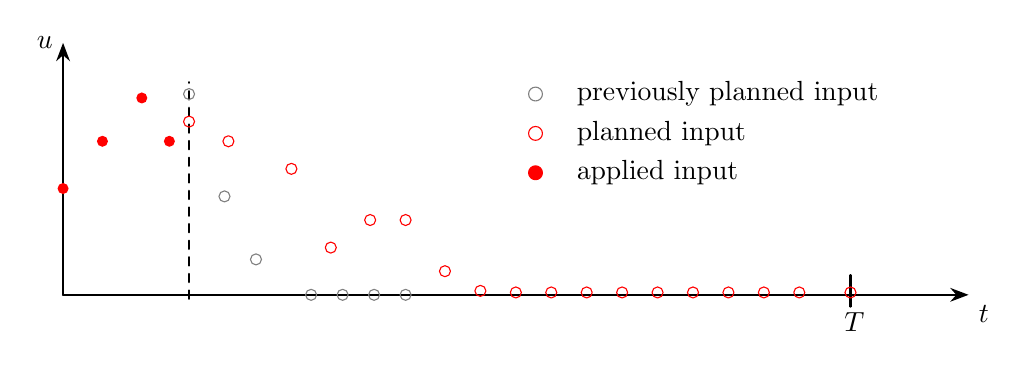
\begin{tikzpicture}[>=Stealth, line cap=round, line join=round, scale=1.0]

    % Axes
    \draw[->, thick] (0,0) -- (11.5,0) node[below right] {$t$};
    \draw[->, thick] (0,0) -- (0,3.2) node[left] {$u$};

    % Horizon marker
    \draw[dashed, thick] (1.6,-0.05) -- (1.6,2.7);

    % T mark
    \draw[thick] (10.0,-0.15) -- (10.0,0.25);
    \node[below] at (10.05,-0.1) {$T$};

    % Legend
    \node[draw=gray, circle, minimum size=5pt, inner sep=0pt] at (6.0,2.55) {};
    \node[anchor=west] at (6.4,2.55) {previously planned input};

    \node[draw=red, circle, minimum size=5pt, inner sep=0pt] at (6.0,2.05) {};
    \node[anchor=west] at (6.4,2.05) {planned input};

    \node[fill=red, draw=red, circle, minimum size=5pt, inner sep=0pt] at (6.0,1.55) {};
    \node[anchor=west] at (6.4,1.55) {applied input};

    % Previously planned input (gray open circles)
    \foreach \x/\y in {
        1.6/2.55,
        2.05/1.25,
        2.45/0.45,
        3.15/0.00,
        3.55/0.00,
        3.95/0.00,
        4.35/0.00
    }{
        \draw[gray] (\x,\y) circle (0.07);
    }

    % Planned input (red open circles)
    \foreach \x/\y in {
        1.6/2.20,
        2.1/1.95,
        2.9/1.60,
        3.4/0.60,
        3.9/0.95,
        4.35/0.95,
        4.85/0.30,
        5.3/0.05,
        5.75/0.03,
        6.2/0.03,
        6.65/0.03,
        7.1/0.03,
        7.55/0.03,
        8.0/0.03,
        8.45/0.03,
        8.9/0.03,
        9.35/0.03,
        10.0/0.03
    }{
        \draw[red] (\x,\y) circle (0.07);
    }

    % Applied input (red filled circles)
    \foreach \x/\y in {
        0.0/1.35,
        0.5/1.95,
        1.0/2.50,
        1.35/1.95
    }{
        \fill[red] (\x,\y) circle (0.07);
    }

\end{tikzpicture}
\caption{Receding-horizon update of the input sequence: previously planned inputs are shifted, a new optimal input sequence is computed based on the current state.}
\label{fig:mpc_01}
\end{figure}

\begin{figure}[!ht]
\centering
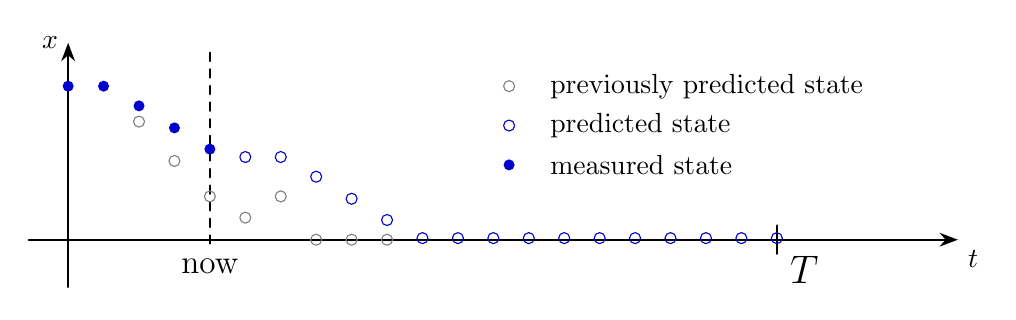
\begin{tikzpicture}[>=Stealth, line cap=round, line join=round, scale=1.0]
    % Axes
    \draw[->, thick] (0,-0.6) -- (0,2.5) node[left] {$x$};
    \draw[->, thick] (-0.5,0) -- (11.3,0) node[below right] {$t$};

    % "now" dashed line
    \draw[dashed, thick] (1.8,-0.05) -- (1.8,2.4);
    \node[below] at (1.8,-0.12) {\large now};

    % Horizon marker T
    \draw[thick] (9.0,-0.18) -- (9.0,0.18);
    \node[below] at (9.35,-0.08) {\Large $T$};

    % Legend
    \draw[gray] (5.6,1.95) circle (0.07);
    \node[anchor=west] at (6.0,1.95) {previously predicted state};

    \draw[blue!80!black] (5.6,1.45) circle (0.07);
    \node[anchor=west] at (6.0,1.45) {predicted state};

    \fill[blue!80!black] (5.6,0.95) circle (0.07);
    \node[anchor=west] at (6.0,0.95) {measured state};

    % Previously predicted state (gray open circles)
    \foreach \x/\y in {
        0.90/1.5,
        1.35/1,
        1.80/0.55,
        2.25/0.28,
        2.70/0.55,
        3.15/0.00,
        3.60/0.00,
        4.05/0.00
    }{
        \draw[gray] (\x,\y) circle (0.07);
    }

    % Predicted state (blue open circles)
    \foreach \x/\y in {
        2.25/1.05,
        2.70/1.05,
        3.15/0.80,
        3.60/0.52,
        4.05/0.25,
        4.50/0.02,
        4.95/0.02,
        5.40/0.02,
        5.85/0.02,
        6.30/0.02,
        6.75/0.02,
        7.20/0.02,
        7.65/0.02,
        8.10/0.02,
        8.55/0.02,
        9.00/0.02
    }{
        \draw[blue!80!black] (\x,\y) circle (0.07);
    }

    % Measured state (blue filled circles)
    \foreach \x/\y in {
        0.00/1.95,
        0.45/1.95,
        0.90/1.70,
        1.35/1.42,
        1.80/1.15
    }{
        \fill[blue!80!black] (\x,\y) circle (0.07);
    }

\end{tikzpicture}
\caption{Receding-horizon update of the state trajectory: previously predicted states are corrected using the measured state at the current time, and a new optimal state trajectory is predicted over the horizon.}
\label{fig:mpc_02}
\end{figure}

The idea that emerges from this discussion is to solve the optimization problem in a \textbf{receding horizon} fashion. At each time step, we solve a finite-horizon optimal control problem of length $T$, and apply only the first control input of the optimal sequence (see Figure \ref{fig:mpc_03}).\\
At the next time step, the new state is measured, and the optimization problem is solved again with the updated initial condition. If the system is time-invariant, the optimization problem remains the same at each time step, except for the initial state. The corresponding predicted state evolution over the horizon is illustrated in Figure \ref{fig:mpc_04}.\\

\begin{figure}[!ht]
\centering
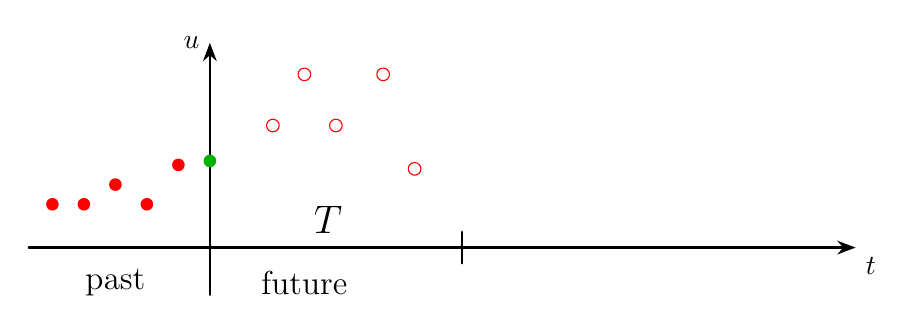
\begin{tikzpicture}[>=Stealth, line cap=round, line join=round, scale=1.0]
    % Axes
    \draw[->, thick] (-2.3,0) -- (8.2,0) node[below right] {$t$};
    \draw[->, thick] (0,-0.6) -- (0,2.6) node[left] {$u$};

    % Horizon marker T
    \draw[thick] (3.2,-0.2) -- (3.2,0.2);
    \node at (1.5,0.35) {\Large $T$};

    % Labels past / future
    \node at (-1.2,-0.45) {\large past};
    \node at (1.2,-0.45) {\large future};

    % Applied inputs (past - red filled)
    \foreach \x/\y in {
        -2.0/0.55,
        -1.6/0.55,
        -1.2/0.80,
        -0.8/0.55,
        -0.4/1.05
    }{
        \fill[red] (\x,\y) circle (0.08);
    }

    % Current input at time 0 (highlighted)
    \fill[green!70!black] (0,1.10) circle (0.08);

    % Planned inputs (future - red open)
    \foreach \x/\y in {
        0.8/1.55,
        1.2/2.20,
        1.6/1.55,
        2.2/2.20,
        2.6/1.00
    }{
        \draw[red] (\x,\y) circle (0.08);
    }

\end{tikzpicture}
\caption{Finite-horizon input sequence in receding horizon control: at the current time, an optimal sequence of future inputs over a horizon of length $T$ is computed, while past inputs are fixed.}
\label{fig:mpc_03}
\end{figure}

\begin{figure}[!ht]
\centering
\begin{tikzpicture}[>=Stealth, line cap=round, line join=round, scale=1.0]

    % Axes
    \draw[->, thick] (-2.3,0) -- (8.7,0) node[below right] {$t$};
    \draw[->, thick] (0,-0.6) -- (0,2.6) node[left] {$x$};

    % Labels past / future
    \node at (-1.2,-0.45) {\large past};
    \node at (1.2,-0.45) {\large future};

    % Horizon marker T
    \draw[thick] (3.2,-0.2) -- (3.2,0.2);
    \node at (1.5,0.35) {\Large $T$};

    % Measured states (past - filled blue)
    \foreach \x/\y in {
        -2.0/1.4,
        -1.5/2.0,
        -1.0/1.4,
        -0.5/1.4,
        0.0/2.0
    }{
        \fill[blue!80!black] (\x,\y) circle (0.08);
    }

    % Predicted states (future - open blue)
    \foreach \x/\y in {
        0.5/2.0,
        1.0/1.4,
        1.5/0.9,
        2.0/0.5,
        2.5/0.0
    }{
        \draw[blue!80!black] (\x,\y) circle (0.08);
    }

\end{tikzpicture}
\caption{Finite-horizon state prediction in receding horizon control: starting from the current state, future states are predicted over a horizon of length $T$ using the planned input sequence.}
\label{fig:mpc_04}
\end{figure}

Thus the following scheme defines the receding horizon control strategy, also known as \textbf{Model Predictive Control (MPC)}:
\begin{enumerate}
\item At time $t$, measure the current state $x_t$.
\item Solve the finite-horizon optimal control problem with initial state $x_t$ to obtain the optimal input sequence $u_t, u_{t+1}, \ldots, u_{t+T-1}$.
\item Apply the first control input $u_t$ to the system.
\item Increment time $t \leftarrow t+1$ and repeat from step 1.
\end{enumerate}

The resulting \textbf{open-loop optimal control problem} corresponds to a \textit{parametric
optimization problem} parametrized in the \textcolor{red}{initial state x}.
\begin{theorembox}[Parametric optimization problem ]
$u^*(x)$ is determined by\footnote{Notation: $k$ is the index for the optimization problem, while $t$ is the index for the time steps of the system.}
\begin{align*}
    \min_{\mathbf{u},\mathbf{x}} &\sum_{k=0}^{T-1} \left( x_k^\top Q x_k + u_k^\top R u_k \right) + x_T^\top S x_T\\
    \text{s.t.} \quad & x_{k+1} = A x_k + B u_k\\
    & \textcolor{red}{x_0 = x} \\
    & x_k \in \mathcal{X}_k \\
    & u_k \in \mathcal{U}_k
\end{align*}
\end{theorembox}

The parametric nature of the problem immediately raises the question of whether the resulting control strategy is \emph{feedforward} or \emph{feedback}. Although the optimization problem computes an open-loop input sequence, the receding horizon implementation introduces feedback implicitly. Indeed, at each time step the optimization problem is solved using the current state $x_t$, and only the first input of the optimal sequence is applied. Therefore, the implemented control law can be written as
\[
u_t = u^*(x_t),
\]
which defines a \textbf{state-feedback control law}. One can have a visual intuition of this feedback structure by looking at the block diagram in Figure \ref{fig:mpc_05}.
\begin{figure}[!ht]
\centering
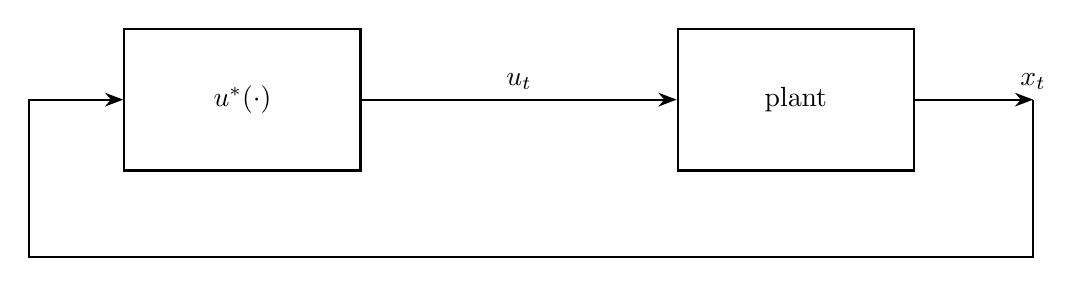
\begin{tikzpicture}[
    >=Stealth,
    block/.style={draw, thick, minimum width=3cm, minimum height=1.8cm},
    node distance=4cm
]

\node[block] (controller) {$u^*(\cdot)$};
\node[block, right=of controller] (plant) {plant};

\draw[->, thick] (controller.east) -- node[above] {$u_t$} (plant.west);
\draw[->, thick] (plant.east) -- ++(1.5,0) node[above] {$x_t$};

\coordinate (out) at ($(plant.east)+(1.5,0)$);
\coordinate (low) at ($(out)+(0,-2)$);
\coordinate (leftlow) at ([xshift=-1.2cm]controller.west |- low);
\coordinate (leftmid) at ([xshift=-1.2cm]controller.west);

\draw[->, thick]
    (out) -- (low) -- (leftlow) -- (leftmid) -- (controller.west);

\end{tikzpicture}

\caption{Block diagram of the MPC control scheme}
\label{fig:mpc_05}
\end{figure}

We can establish some properties about this optimization problem:
\begin{itemize}
    \item Under \textbf{continuity} assumptions on the cost and the dynamics, the minimum cost is a constinuous function of the initial state $x$.
    \item Under \textbf{compactness} assumptions on the constraints, the parametric optimization problem admits a solution for all $x$ in the feasible set.
    \item The map $x \mapsto u^*(x)$ is not necessarily continuos for a general cost function
\end{itemize}
In the case of linear dynamics, quadratic cost, and convex constraints, the optimization problem is a convex quadratic program (QP) parametrized in the initial state $x$. In this case, the map $x \mapsto u^*(x)$ is piecewise affine and continuous. However, in general, the control law induced by MPC can be nonlinear and non-smooth.
\begin{theorembox}[MPC control law]
As a consequence, MPC can be interpreted as a \textbf{memory-less, nonlinear, time-invariant feedback control law}. The nonlinearity arises from the presence of constraints, even when the system dynamics are linear and the cost is quadratic.\\
\end{theorembox}

A natural question is whether MPC can achieve \emph{perfect tracking}, i.e., zero steady-state error. In general, this is not guaranteed without additional design choices (e.g., terminal ingredients or disturbance modeling), since the controller repeatedly solves a finite-horizon problem and does not explicitly enforce asymptotic properties beyond the prediction horizon.
To better understand the relation between MPC and the finite-horizon optimal control problem, consider the following example:
\paragraph{Example}
\begin{align*}
\min_{\mathbf{x},\mathbf{u}} \quad & \sum_{t=0}^{T-1} a^t |u_t| + |x_T|^2, \quad |a| < 1 \\
\text{s.t.} \quad & x_{t+1} = x_t + u_t.
\end{align*}

Two different questions can be asked:
\begin{enumerate}
    \item What is the optimal open-loop solution $(\mathbf{x}^*, \mathbf{u}^*)$?
    \item What is the MPC feedback law $x \mapsto u^*(x)$ obtained by solving the problem in a receding horizon fashion?
\end{enumerate}
To solve this we observe that the cost is not quadratic and that the cost of applying inouts is discounted over time. Furthermore the state is penalized only at the end of the horizon.\\
Thus the optimal solution is to simply wait for the last time step and then apply $u_{T} = -x_{T}$, which yields a cost of $|x_0|^2$.\\
In contrast, the MPC feedback law is given by the control law $x \mapsto u^*(x)=0$.\\
A key observation is that the optimal trajectory associated with the finite-horizon problem is, in general, \textbf{never realized in closed loop}, even in the absence of disturbances or model mismatch. This is because at each time step the optimization problem is re-solved with a shifted horizon, leading to a different optimal sequence than the one computed previously.
$\blacksquare$

\medskip

Consider now the unconstrained linear-quadratic problem:
\begin{align*}
\min_{\mathbf{x},\mathbf{u}} \quad & \sum_{t=0}^{T-1} \left( x_t^\top Q x_t + u_t^\top R u_t \right) + x_T^\top S x_T, \quad Q,S \succeq 0,\; R \succ 0 \\
\text{s.t.} \quad & x_{t+1} = A x_t + B u_t.
\end{align*}
\textbf{Finite-time LQR} yields a time-varying linear feedback law
\begin{align*}
    u_t &= \Gamma_t x_t\\
    \Gamma_t &= -(R + B^\top P_{t+1} B)^{-1} B^\top P_{t+1} A
\end{align*}
where the matrices $P_t$ are computed backward in time. The control gain explicitly depends on time through $P_{t+1}$.\\
In contrast, \textbf{MPC} repeatedly solves the same finite-horizon problem at each time step. As a result, the applied control law is
\[
u_t = \Gamma_0 x_t,
\]
where $\Gamma_0$ is the gain associated with the first step of the horizon. Hence, MPC induces a \textbf{linear time-invariant} feedback law.\\
More explicitly, at time $t=0$ both approaches yield the same control input:
\[
u_0^{\text{MPC}} = -(R + B^\top P_1 B)^{-1} B^\top P_1 A x_0 = u_0^{\text{LQR}}.
\]
However, at the next time step a discrepancy appears. Finite-time LQR applies
\[
u_1^{\text{LQR}} = \textcolor{blue}{-(R + B^\top P_2 B)^{-1} B^\top P_2 A} x_1,
\]
while MPC recomputes the problem and applies again
\[
u_1^{\text{MPC}} = {-(R + B^\top \textcolor{red}{P_1} B)^{-1} B^\top \textcolor{red}{P_1} A} x_1.
\]
Therefore, even in the unconstrained case, MPC does not reproduce the finite-horizon optimal control sequence beyond the first step.

\subsection{Implementation of MPC}
The implementation of MPC requires solving an optimization problem at each time step. We show two main approaches to implement MPC:
\begin{enumerate}
    \item Compute the \textbf{function} $u^*(\cdot)$ \textbf{offline}, and then evaluate it online at each time step.
    \begin{itemize}
        \item It is extremely complex to solve with exception of very few cases
        \item Abundant offline computational resources are required 
        \item Large memory is required to store the function $u^*(\cdot)$
    \end{itemize}
    \item Compute the \textbf{value} of the function $U^*(\cdot)$ \textbf{online} at each time step by solving the optimization problem.
    \begin{itemize}
        \item It is ogten a tractable optimization problem.
        \item It has limited time to perform computation online.
    \end{itemize}
\end{enumerate}

\subsubsection{Explicit MPC}

Explicit MPC corresponds to the first implementation strategy: instead of solving the optimization problem online at each sampling instant, we try to compute the feedback law$ x \mapsto u^*(x) $
offline.\\
We have already seen one important case. In the \textbf{unconstrained linear MPC} case, the optimizer is simply the first element of the finite-horizon LQR solution. Therefore, the applied input can be written as
\[
u_t = u^*(x_t)=\Gamma_0 x_t,
\]
so the control law is linear.\\

The natural question is what happens when \emph{constraints} are introduced. Consider the standard constrained linear MPC problem

\begin{theorembox}[Linear MPC with linear constraints]
\begin{align*}
\min_{\mathbf{u},\mathbf{x}} \quad &
\sum_{k=0}^{T-1}\left(x_k^\top Q x_k + u_k^\top R u_k\right) + x_T^\top S x_T \\
\text{s.t.}\quad
& x_{k+1}=Ax_k+Bu_k, \qquad k=0,\dots,T-1, \\
& x_0=x, \\
& x_k \in \mathcal{X}, \qquad \mathcal{X}=\{x \in \mathbb{R}^n : Cx \le d\}, \\
& u_k \in \mathcal{U}, \qquad \mathcal{U}=\{u \in \mathbb{R}^m : Eu \le f\},
\end{align*}
with $ Q,S \succeq 0, \qquad R \succ 0 $.\\
This is the most common MPC formulation: linear dynamics, quadratic cost, and polyhedral state/input constraints.
\end{theorembox}
This problem is a \textbf{convex quadratic program} parametrized by the initial state $x$. In general, the optimizer is no longer globally linear. However, due to the quadratic cost and linear constraints, it still has a very specific structure: the explicit MPC law turns out to be \textbf{piecewise affine}. The idea is best understood through a very simple example.

\paragraph{Example}
Consider a scalar integrator with horizon $T=1$:
\begin{align*}
\min_{u_0,x_1} \quad & u_0^2 + x_1^2 \\
\text{s.t.}\quad & x_1 = x_0 + u_0, \\
& x_1 \le 1.
\end{align*}

This example is useful because:
\begin{itemize}
    \item it is a quadratic problem with a linear constraint,
    \item it is parametrized by the current state $x_0$,
    \item the equality constraint allows us to eliminate the variable $x_1$,
    \item the problem is convex, hence the KKT conditions are necessary and sufficient.
\end{itemize}
Using the model equation $x_1=x_0+u_0$, we can eliminate $x_1$ and rewrite the problem as
\[
\min_{u_0} f(u_0)
\qquad \text{s.t.} \qquad g(u_0)\le 0,
\]
where
\begin{align*}
f(u_0) &= u_0^2 + (x_0+u_0)^2, \\
g(u_0) &= x_0 + u_0 - 1.
\end{align*}
The derivatives are
\begin{align*}
\nabla f(u_0) &= 4u_0 + 2x_0, \\
\nabla g(u_0) &= 1.
\end{align*}

\begin{theorembox}[KKT conditions for one inequality constraint]
For a problem of the form
\[
\min_x f(x)
\qquad \text{s.t.}\qquad g(x)\le 0,
\]
the KKT conditions are
\begin{align*}
\nabla f(x)+\mu \nabla g(x) &= 0, \qquad \mu \ge 0,\\
g(x) &\le 0,\\
\mu\, g(x) &= 0.
\end{align*}
The last relation is the \emph{complementary slackness} condition.
\end{theorembox}

Applying the KKT conditions to the problem gives
\begin{align*}
4u_0 + 2x_0 + \mu &= 0, \qquad \mu \ge 0, \\
x_0 + u_0 - 1 &\le 0, \\
\mu(x_0 + u_0 - 1) &= 0.
\end{align*}

The complementary slackness condition implies that two cases are possible.

\paragraph{Case 1: inactive constraint.}
Assume first that the inequality is inactive, so
\[
\mu = 0.
\]
Then stationarity becomes
\[
4u_0 + 2x_0 = 0,
\]
hence
\[
u_0 = -\frac{x_0}{2}.
\]
To check whether this candidate is feasible, we substitute it into the constraint:
\[
x_0 + u_0 - 1 = x_0 - \frac{x_0}{2} - 1 = \frac{x_0}{2} - 1.
\]
Therefore feasibility requires
\[
\frac{x_0}{2} - 1 \le 0
\qquad \Longleftrightarrow \qquad
x_0 \le 2.
\]
So, for all initial states satisfying $x_0 \le 2$, the optimal input is
\[
u_0^* = -\frac{x_0}{2}.
\]

\paragraph{Case 2: active constraint.}
Assume now that the inequality is active, so
\[
x_0 + u_0 - 1 = 0.
\]
Then
\[
u_0 = 1 - x_0.
\]
Substituting this into the stationarity condition,
\[
4u_0 + 2x_0 + \mu = 0,
\]
we obtain
\[
\mu = -4u_0 - 2x_0 = -4(1-x_0)-2x_0 = 2x_0 - 4.
\]
Since $\mu \ge 0$, this case is valid only if
\[
2x_0 - 4 \ge 0
\qquad \Longleftrightarrow \qquad
x_0 \ge 2.
\]
Hence, for all $x_0 \ge 2$, the optimal input is
\[
u_0^* = 1 - x_0.
\]

Combining the two cases, the explicit solution is
\begin{theorembox}[Explicit solution of the toy MPC problem]
\[
u_0^*(x_0)=
\begin{cases}
-\dfrac{x_0}{2}, & x_0 \le 2, \\[1ex]
1-x_0, & x_0 \ge 2.
\end{cases}
\]
\end{theorembox}

This example shows the main structural property of explicit MPC:
\begin{itemize}
    \item the control law is \textbf{continuous},
    \item the control law is \textbf{piecewise affine},
    \item each affine expression is valid in a region where the same set of constraints is active.
\end{itemize}

The reason is the following. Once the active constraints are known, the KKT conditions reduce to a linear system in the decision variables and the multipliers. Solving that linear system gives an optimizer that depends \emph{affinely} on the parameter $x$. When the active set changes, a different affine expression is obtained. Therefore, the state space is partitioned into regions, and on each region the controller is affine.\\

Although the explicit solution is conceptually appealing, it becomes difficult to use in large problems. In practice:
\begin{itemize}
    \item there may be tens or hundreds of constraints,
    \item the number of regions may become very large,
    \item the offline computation required to determine all regions can be very long,
    \item even online, one must determine in which region the current state lies before evaluating the affine law.
\end{itemize}
As a consequence, explicit MPC is mainly attractive when the system dimension is small and the sampling time is so short that solving a quadratic program online would be too expensive. For larger systems, the most common approach is instead to solve the MPC optimization problem online at each sampling instant.

\subsection{Stability}

A useful way to think about MPC is as a \emph{feedback design tool}. Once the prediction horizon $T$ and the weights $Q,R,S$ are chosen, the receding-horizon implementation induces a control law of the form
\[
u_t = u^*(x_t).
\]
Even though the optimization problem computes an open-loop input sequence, only the first input is applied and the problem is solved again at the next time step. Therefore, the implemented controller is a \textbf{static, time-invariant, nonlinear feedback law}. The nonlinearity does not necessarily come from the dynamics; it already appears because of the repeated constrained optimization.\\
From this perspective, the main question is no longer only how to solve the optimization problem, but whether the resulting closed-loop system is stable. There are two conceptually different ways to approach this question. The first is an \emph{analysis} point of view: one tries to compute the control law $u^*(\cdot)$ explicitly and then study the stability of the closed-loop dynamics. In general, this is difficult, because the MPC law can be piecewise affine or more generally nonlinear and non-smooth. The second is a \emph{design} point of view: instead of computing the feedback law explicitly, one looks for conditions on the design parameters $T,Q,R,S$ that guarantee closed-loop stability directly. This is the more useful viewpoint in practice.\\

To study stability, the standard tool is Lyapunov analysis. Consider a discrete-time system
\[
x_{t+1}=f(x_t),
\]
and suppose that the origin $x=0$ is an equilibrium, that is, $f(0)=0$.

\begin{theorembox}[Stable equilibrium]
The equilibrium $x=0$ is said to be \textbf{stable} if
\[
\forall \varepsilon > 0, \ \exists \delta > 0 \text{ such that } \norm{x_0}<\delta
\ \Longrightarrow\ 
\norm{x_t}<\varepsilon \quad \forall t\geq 0.
\]
In words, if the initial condition is sufficiently close to the equilibrium, then the entire trajectory remains close to it for all future times.
\end{theorembox}

Stability alone only guarantees that trajectories do not move far away from the equilibrium. A stronger notion is asymptotic stability, which additionally requires convergence to the equilibrium.

\begin{theorembox}[Asymptotically stable equilibrium]
The equilibrium $x=0$ is \textbf{asymptotically stable} if it is stable and
\[
\lim_{t\to\infty}\norm{x_t}=0.
\]
Hence, trajectories starting sufficiently close to the origin remain close to it and eventually converge to it.
\end{theorembox}

The classical criterion to prove asymptotic stability is based on a Lyapunov function.

\begin{theorembox}[Lyapunov theorem for discrete-time systems]
Assume there exists a real-valued function $W:\mathbb{R}^n\to\mathbb{R}$ such that
\begin{align*}
W(0) &= 0,\\
W(x) &> 0 \qquad \forall x\neq 0,\\
W(f(x)) &< W(x) \qquad \forall x\neq 0.
\end{align*}
Then the equilibrium $x=0$ is asymptotically stable.
\end{theorembox}

The idea is simple: $W$ plays the role of an energy-like quantity. It is zero only at the equilibrium, positive everywhere else, and strictly decreases along the closed-loop trajectories. Therefore, the system is forced to move toward the origin.\\

This Lyapunov viewpoint explains why stability is relatively transparent for \emph{infinite-horizon} MPC. Suppose that, at time $t$, the controller computes an input sequence that minimizes the infinite-horizon cost
\[
V_t^\infty(x,\mathbf{u}) = \sum_{k=t}^{\infty} g_k(x_k,u_k),
\]
subject to the system dynamics. If the minimum is attained, it is natural to define the optimal value function
\[
W(x) = \min_{\mathbf{u}} V_t^\infty(x,\mathbf{u}).
\]
Now comes the key observation. By Bellman's principle of optimality, if an input sequence is optimal from time $t$, then its tail is optimal from time $t+1$ onward. In other words, after applying the first optimal input $u^*(x_t)$ and reaching the next state $x_{t+1}$, the remaining part of the optimal sequence is still optimal for the optimization problem starting at $t+1$. As a consequence, along the closed-loop trajectory one obtains
\[
W(x_{t+1}) = W(x_t) - g_t(x_t,u^*(x_t)).
\]
Therefore, if the stage cost satisfies suitable positivity properties, for example if
\[
g_t(x_t,u_t) > 0 \qquad \text{for all } x_t\neq 0,
\]
then
\[
W(x_{t+1}) < W(x_t) \qquad \text{for all } x_t\neq 0.
\]
This means that the optimal value function is a natural Lyapunov candidate for the closed-loop system. Under reasonable assumptions, it follows that the origin is asymptotically stable.\\

This argument is very elegant, but it also hides some subtleties. First, an infinite-horizon MPC problem is infinite-dimensional, so from a computational viewpoint it is not directly implementable as stated. Second, one is implicitly assuming that the global minimum exists and is attained. Third, the stage cost must satisfy suitable properties so that the value function is positive definite and decreases strictly along the closed loop. These requirements are analogous in spirit to the assumptions encountered in infinite-horizon LQR.\\

The situation changes significantly for \emph{finite-horizon} MPC. In that case, the same Lyapunov argument does not apply automatically. At time $t$, the controller minimizes a cost over the interval $[t,t+T]$. At time $t+1$, however, the optimization problem is not simply the tail of the previous one: the first stage cost has disappeared, but a new term has entered at the end of the horizon. Therefore, the controller at time $t+1$ is minimizing a \emph{different} objective. As a result, the optimizer changes, and the finite-horizon value function is not automatically decreasing along the closed-loop trajectory.

This is the fundamental reason why closed-loop stability is immediate for infinite-horizon optimal control, but not for finite-horizon receding-horizon MPC. For finite-horizon MPC, stability must be enforced through additional design choices. This will be the starting point for the next part of the discussion.
\newpage

\section{Economic MPC}
\subsection{From setpoint tracking to nonzero steady states}
In the previous chapters we have always implicitly assumed that we are regulating the steady state $x_S = 0$, $u_S = 0$.\\
However, in many applications we are interested in regulating to a nonzero setpoint, or even tracking a time-varying reference trajectory. In particular, we typically want the plant to operate at a desired working point $x_S \neq 0$, and we can allow for a constant input $u_S$ that compensates for constant disturbances.
\subsubsection{Computation of a feasible steady-state target}
If a desired equilibrium point $(x_S,u_S)$ is known, it satisfies
$$
x_S = A x_S + B u_S.
$$
In this case, MPC can be used to stabilize the system around this point by introducing the shifted variables
$$
\tilde{x}_k = x_k - x_S, \qquad \tilde{u}_k = u_k - u_S.
$$
Substituting into the system dynamics $x_{k+1} = A x_k + B u_k$, we obtain
$$
\tilde{x}_{k+1} = A \tilde{x}_k + B \tilde{u}_k,
$$
which has exactly the same form as the original system. Therefore, in the new coordinates, the regulation problem becomes a standard stabilization problem around the origin.\\
The finite-horizon MPC cost can then be written as
$$
V(x_0) = \min_{\mathbf{\tilde{x}},\mathbf{\tilde{u}}} \sum_{k=0}^{K-1} \left( \tilde{x}_k^\top Q \tilde{x}_k + \tilde{u}_k^\top R \tilde{u}_k \right) + \tilde{x}_K^\top S \tilde{x}_K.
$$
For linear systems, this change of variables is \textbf{inconsequential}, since it does not modify the structure of the optimal control problem: the dynamics remain linear, the cost remains quadratic, and the constraints (if any) remain affine. As a result, regulating the system to $(x_S,u_S)$ is equivalent to regulating the shifted system to the origin.\\

\subsubsection{Computation of the steady-state target}
But how do we decide the steady state $(x_S,u_S)$ to which we want to regulate? In some cases, this may be given by the problem specification, e.g., if we want to track a reference trajectory. In other cases, it can be derived from first principles, e.g., by solving the steady-state equations of the system.\\
In other cases, specifications indicate a desidered steady state $(x_{\text{spec},u_{\text{spec}}})$, but the system cannot be stabilized around it. In this case, we can use MPC to find the closest stabilizable point to the desired one, by solving the following optimization problem:
\[
\begin{aligned}
\min_{x_S, u_S} \quad & \| x_S - x_{\text{spec}} \|_{Q_S}^2 + \| u_S - u_{\text{spec}} \|_{R_S}^2 \\
\text{subject to} \quad & \begin{bmatrix}I - A & -B\end{bmatrix}\begin{bmatrix}
x_S \\ u_S
\end{bmatrix} = 0\\
& (x_S, u_S) \in \mathcal{X} \times \mathcal{U},
\end{aligned}
\]
where $\mathcal{X}$ and $\mathcal{U}$ are the state and input constraint sets, respectively. The condition $\begin{bmatrix}I - A & -B\end{bmatrix}\begin{bmatrix}x_S \\ u_S
\end{bmatrix} = 0$ ensures that the chosen point is an equilibrium of the system, while the cost function penalizes deviations from the desired specifications.\\
This optimization problem is typically \textbf{solved offline} and serves to compute a feasible and stabilizable steady-state target $(x_S,u_S)$. The resulting pair is then used as the reference for the MPC regulator, which is responsible for driving the system to this point while satisfying constraints.
\subsection{Motivation for economic MPC}
Many modern control problems present \textbf{complex performance metrics} that cannot be easily captured by a quadratic cost function. For example, in chemical processes, the economic performance of the system may depend on nonlinear functions of the state and input variables, such as production rates, energy consumption, or profit margins. In such cases, we can use \textbf{economic MPC}, which allows for more general cost functions that directly reflect the economic objectives of the system.\\

Thus, let $\ell(x,u)$ be a general stage cost function that captures the economic performance of the system like economic losses, energy use , cost of material, etc. The economic MPC problem assumes that
\begin{itemize}
    \item $\ell(x,u)$ is a \textbf{continuos} function;
    \item $\ell(x,u)$ is \textbf{lower bounded} in the domain
\end{itemize}
While remember that in MPC we were assuming that
\begin{itemize}
    \item $g(x_S,u_S) = 0$ (i.e., the system is at equilibrium at the desired setpoint);
    \item $g(x,u)\geq 0$
    \item $g(x,u)$ is radially unbounded, continuos, zero at the origin, and strictly increasing.
    \item e.g. $g(x,u) = x^\top Q x + u^\top R u$.
\end{itemize}
\subsubsection{Steady-state economic optimization plus tracking MPC}
One possible approach is to \textbf{separate the economic objective from the dynamic control problem}. In particular, the economic cost is handled at the steady-state level, while MPC is used to steer the system toward the corresponding optimal operating point.\\
Given a general stage cost $\ell(x,u)$, we first define the \textbf{steady-state optimization problem}
\[
\begin{aligned}
\min_{x_S,u_S} \quad & \ell(x_S,u_S) \\
\text{subject to} \quad & x_S = f(x_S,u_S), \\
& (x_S,u_S) \in \mathcal{X} \times \mathcal{U}.
\end{aligned}
\]
This problem \textbf{determines the economically optimal equilibrium of the system}.\\

The resulting pair $(x_S,u_S)$ is then used as a reference for the MPC controller, which is designed to track this steady state using a standard quadratic cost. In this way, the economic objective is indirectly enforced through steady-state optimization, while the MPC ensures closed-loop stability and constraint satisfaction.\\

This approach is typically implemented by solving the steady-state optimization problem offline, or at a slower time scale than the MPC loop. However, this separation introduces some limitations. The closed-loop trajectory is generally \textbf{suboptimal from an economic point of view}, since the stage cost $\ell(x,u)$ is not minimized during transients. Moreover, the controller cannot exploit transient behavior to improve performance, and its response to disturbances may be economically inefficient. On the other hand, the resulting MPC problem remains a standard linear-quadratic program, which is computationally efficient and well understood.\\

\subsection{Economic MPC formulation}
\subsubsection{Dynamic economic optimization}
An alternative approach is to \textbf{incorporate the economic objective} directly into the dynamic optimization problem. This leads to the formulation of \textbf{economic MPC}, in which the stage cost $\ell(x,u)$ is optimized along the entire predicted trajectory:
\[
V(x) = \min_{\mathbf{x},\mathbf{u}} \sum_{k=0}^{K-1} \ell(x_k,u_k)
\]
subject to
\[
x_{k+1} = f(x_k,u_k), \quad x_0 = x, \quad x_k \in \mathcal{X}, \quad u_k \in \mathcal{U}.
\]
In contrast to the previous approach, there is \textbf{no separation} between steady-state optimization and tracking. The controller directly optimizes the economic performance over the prediction horizon, resulting in a \emph{single time-scale} scheme in which both transient and steady-state behavior are determined simultaneously.\\

As a consequence, the controller computes control actions that generate an economically optimal trajectory, rather than simply driving the system toward a precomputed steady state. In particular, the optimal operation may not correspond to a fixed equilibrium, and the controller may intentionally exploit transient behavior if this improves the overall performance.\\
This increased flexibility comes at the price of a \textbf{more challenging optimization problem}. Since the cost $\ell(x,u)$ is in general nonlinear and not necessarily convex, the resulting optimal control problem may be non-convex and harder to solve in real time. Moreover, standard quadratic Lyapunov arguments used in tracking MPC no longer apply directly, and additional conditions are required to guarantee stability.\\

On the other hand, economic MPC is particularly well suited for nonlinear systems and applications in which performance is naturally described by non-quadratic criteria, such as energy efficiency or economic profit. In these cases, directly optimizing $\ell(x,u)$ allows the controller to fully exploit the system dynamics and constraints to achieve improved closed-loop performance.\\

A \textbf{key issue} with economic MPC arises from the fact that the stage cost $\ell(x,u)$ is not designed to enforce convergence to a steady state. In particular, it may happen that there exist pairs $(x,u)$ that are not equilibria of the system, i.e.,
\[
x \neq f(x,u),
\]
for which
\[
\ell(x,u) < \ell(x_S,u_S),
\]
where $(x_S,u_S)$ is an optimal steady state.\\
This situation is not pathological; on the contrary, it is quite common in practice. Since $\ell(x,u)$ reflects instantaneous economic performance, \textbf{it may be advantageous for the system to operate away from equilibrium}, for instance by exploiting transient dynamics or time-varying operating conditions.\\

As a consequence, convergence to a steady state is no longer guaranteed nor even desired in general. The optimal closed-loop behavior may correspond to trajectories that do not settle at an equilibrium, such as periodic or more complex operating regimes.\\
This highlights a \textbf{fundamental difference} with standard tracking MPC: convergence to a steady state is not part of the control specification. Instead, the objective is to optimize economic performance over time, possibly at the expense of steady-state operation.\\

However, this increased flexibility comes with \textbf{important challenges}. First, operating away from equilibrium can lead to behaviors that are harder to analyze and predict. In particular, stability and boundedness of the closed-loop trajectories are not automatically guaranteed. Second, without additional conditions or constraints, the controller may generate trajectories that are economically optimal in the short term but undesirable from a safety or robustness perspective.

\subsubsection{Infinite horizon, finite horizon, and terminal constraints}
A fundamental design choice in economic MPC is the length of the prediction horizon. In principle, the most natural formulation is the infinite-horizon problem
\[
\sum_{k=0}^{\infty} \ell(x_k,u_k),
\]
which directly captures the long-term economic performance of the system.\\
The infinite-horizon formulation has a clear economic interpretation, as it reflects the cumulative cost over an indefinite future. This is particularly meaningful in continuous operation settings, where there is no natural terminal time and performance is evaluated over the long run. Moreover, constraints are enforced over the entire trajectory, which ensures boundedness of the closed-loop system by construction.\\
However, the infinite-horizon problem is infinite-dimensional and therefore computationally intractable in practice. For this reason, it cannot be solved directly in real time.\\

As a result, practical implementations rely on a finite-horizon approximation of the form
\[
\sum_{k=0}^{K-1} \ell(x_k,u_k).
\]
This leads to a tractable optimization problem that can be solved online within the MPC framework.\\
In standard tracking MPC, a finite horizon provides a good approximation of the infinite-horizon problem, since the system is driven toward an equilibrium and the contribution of the tail beyond the horizon can be neglected or approximated. In economic MPC, this argument no longer holds. Since the optimal behavior may not converge to a steady state, the portion of the trajectory beyond the horizon can have a significant impact on performance.\\

This mismatch introduces several potential issues. First, the controller may favor trajectories that yield low cost within the prediction horizon but lead to poor behavior afterward, as future consequences are not accounted for. In particular, the system may move toward regions from which recovery is difficult or expensive, resulting in undesirable or even unstable behavior.\\
Second, feasibility problems may arise at the end of the horizon. Due to state and input constraints, not all states reached within the horizon can be extended to admissible infinite trajectories. This can lead to situations in which the optimization problem becomes infeasible at future time steps.\\

A common approach to mitigate these issues is to augment the finite-horizon problem with a terminal constraint. In particular, one enforces that the predicted trajectory reaches a feasible steady state at the end of the horizon, i.e.,
\[
x_K = x_S, \qquad u_K = u_S,
\]
where $(x_S,u_S)$ is an admissible equilibrium of the system.\\
This modification preserves the computational tractability of the finite-horizon formulation, while introducing a mechanism to guarantee that the predicted trajectory can be extended beyond the horizon in a feasible way. In other words, by constraining the terminal state to an equilibrium, one ensures that there exists a feasible infinite-horizon continuation, thereby recovering \emph{recursive feasibility}.\\

From this perspective, the terminal constraint provides an explicit characterization of what constitutes a feasible infinite-horizon trajectory: a trajectory is admissible if it can be steered to a steady state that satisfies the system dynamics and constraints.\\
However, the introduction of a terminal constraint also raises important questions regarding the resulting closed-loop behavior. In particular, it is no longer immediate whether the closed-loop system is stable, or whether the resulting trajectory achieves optimal economic performance. The terminal constraint enforces convergence to a steady state, which may restrict the ability of the controller to exploit economically favorable transient or non-equilibrium operation.

Finally, it is important to emphasize that, as in any MPC scheme, the closed-loop system does not follow the predicted trajectory exactly. At each time step, only the first control input is applied,
\[
u_k = u^*(x_k),
\]
and the optimization problem is solved again at the next step with updated state information. As a result, the actual closed-loop trajectory is generated by the repeated solution of the finite-horizon problem, and not by the open-loop prediction computed at a single time instant.

\subsection{Illustrative example}
To better illustrate the difference between standard tracking MPC and economic MPC, consider the following linear system
\[
x_{k+1} = A x_k + B u_k, \qquad 
A = \begin{bmatrix} \tfrac{1}{2} & 1 \\ 0 & \tfrac{3}{4} \end{bmatrix}, \quad 
B = \begin{bmatrix} 0 \\ 1 \end{bmatrix},
\]
with input constraint
\[
u \in \mathcal{U} = [-1,1],
\]
and economic stage cost
\[
\ell(x,u) = q^\top x + r u, \qquad 
q = \begin{bmatrix} -2 \\ 2 \end{bmatrix}, \quad r = -10.
\]
\subsubsection{Computation of the optimal steady state}
The first step consists in computing the optimal steady state by solving
\[
\begin{aligned}
\min_{x_S,u_S} \quad & \ell(x_S,u_S) \\
\text{subject to} \quad & x_S = A x_S + B u_S, \\
& u_S \in \mathcal{U}.
\end{aligned}
\]
To find the steady states we need to solve
\[
(I - A )x_S = B u_S,
\]
which gives
\[
\begin{bmatrix}
    \frac{1}{2} & -1 \\
    0 & \frac{1}{4}
\end{bmatrix}
\begin{bmatrix}
x_{S,1} \\ x_{S,2}
\end{bmatrix}
= \begin{bmatrix}0 \\ u_S
\end{bmatrix}
\]
Since the cost is linear and the constraints define a polyhedral set, this is a linear program, and the optimum is attained at an extreme point of the feasible set. Thus we only need to evaluate the cost at the two vertices of the input constraint, which gives
$$\text{if}\; u_S = -1, \quad x_S = \begin{bmatrix} -4 \\ -8 \end{bmatrix}, \quad \ell(x_S,u_S) = 18,$$
$$\text{if}\; u_S = 1, \quad x_S = \begin{bmatrix} 4 \\ 8 \end{bmatrix}, \quad \ell(x_S,u_S) =- 18.$$

The solution $(x_S^*,u_S^*)$ represents the economically optimal equilibrium.
\subsubsection{Tracking MPC versus economic MPC}
Once $(x_S^*,u_S^*)$ is determined, two fundamentally different control strategies can be constructed.\\

In the standard MPC tracking approach, the optimal steady state is used as a reference. Defining the shifted variables
\[
\tilde{x}_k = x_k - x_S^*, \qquad \tilde{u}_k = u_k - u_S^*,
\]
the controller minimizes a quadratic tracking cost of the form
\[
g(\tilde{x},\tilde{u}) = \tilde{x}^\top Q \tilde{x} + \tilde{u}^\top R \tilde{u},
\]
driving the system to $(x_S^*,u_S^*)$ as fast as possible. A terminal constraint $\tilde{x}_K = 0$ (equivalently $x_K = x_S^*$) is typically imposed to ensure stability. The resulting optimization problem is a quadratic program.\\

In contrast, economic MPC directly uses the economic cost in the receding horizon problem:
\[
\min_{\mathbf{x},\mathbf{u}} \sum_{k=0}^{K-1} \ell(x_k,u_k)
\]
subject to
\[
x_{k+1} = A x_k + B u_k, \qquad x_k \in \mathcal{X}, \quad u_k \in \mathcal{U},
\]
together with a terminal constraint $x_K = x_S^*$ to guarantee feasibility. In this case, since both the dynamics and the cost are linear, the resulting problem is a linear program.\\

The key difference between the two approaches lies in the objective being optimized. Tracking MPC enforces convergence to the economically optimal steady state and prioritizes stability and regulation performance, but does not optimize the economic cost during transients. Economic MPC, on the other hand, optimizes the economic objective along the entire trajectory, potentially exploiting transient behavior to improve performance.\\

From a computational perspective, tracking MPC leads to a quadratic program, which is typically well-conditioned and easier to solve reliably in real time. Economic MPC may lead to linear or nonlinear programs depending on the form of $\ell(x,u)$, and can be more challenging, although in this particular example it reduces to a linear program.
\subsection{Closed-loop analysis}
Now we want to analyze the closed loop behavior. In particular we want to understand if the closed loop stability is guaranteed and if the economic cost is minimez.
\subsubsection{Tracking MPC: Lyapunov decrease}
In standard tracking MPC, the terminal constraint plays a crucial role in proving asymptotic stability. Indeed, when the cost is built from a positive definite tracking stage cost
\[
g(\tilde{x},\tilde{u}),
\]
with
\[
g(0,0)=0, \qquad g(\tilde{x},\tilde{u})>0 \quad \text{for } \tilde{x}\neq 0,
\]
the finite-horizon optimal value function can be used as a Lyapunov function for the closed-loop system. The key argument is the same shifted-sequence argument already discussed in the previous chapter. If the optimal predicted trajectory satisfies the terminal constraint
\[
\tilde{x}_K = 0,
\]
then, after applying the first optimal input, a feasible candidate sequence at the next time step is obtained by shifting the previously optimal sequence and appending the equilibrium input $\tilde{u}=0$. Since the appended terminal stage cost is zero, one obtains
\[
W(f(\tilde{x},u_0^*(\tilde{x}))) \leq W(\tilde{x}) - g(\tilde{x},u_0^*(\tilde{x})) \leq W(\tilde{x}),
\]
which shows that $W$ decreases along the closed-loop trajectories and is therefore a valid Lyapunov function.
\subsubsection{Economic MPC: why the value function is not a Lyapunov function}
The natural question is whether the same idea can be applied to economic MPC. Suppose that we consider the finite-horizon economic MPC problem with terminal constraint
\[
x_K = x_S,
\]
where $(x_S,u_S)$ is an admissible steady state. The same shifted-sequence construction remains feasible: after applying the first optimal control input, one can shift the optimal predicted trajectory and append the steady-state input $u_S$ at the end of the horizon. Therefore, feasibility is preserved. However, the cost argument changes in a fundamental way.\\
Indeed, for economic MPC the stage cost is $\ell(x,u)$, which is not positive definite with respect to the steady state and is not, in general, minimized at $(x_S,u_S)$. As a consequence, the shifted-sequence argument only yields
\[
W(f(x,u_0^*(x))) \leq W(x) - \ell(x,u_0^*(x)) + \ell(x_S,u_S).
\]
This inequality is not sufficient to conclude that $W$ decreases. In fact, it may happen that
\[
\ell(x_S,u_S) > \ell(x,u_0^*(x)),
\]
so the right-hand side can be larger than $W(x)$. Therefore, unlike in tracking MPC, the optimal finite-horizon value function is \emph{not} automatically a Lyapunov function for the closed-loop system.\\

This observation has an important conceptual consequence. In economic MPC, asymptotic stability of the steady state is not guaranteed by the terminal constraint alone. The terminal constraint guarantees recursive feasibility, but not necessarily convergence to the equilibrium. This is perfectly consistent with the economic interpretation of the problem: the controller is asked to optimize economic performance, not to minimize the distance from the steady state. If operating away from equilibrium is economically more favorable, then the closed-loop system may prefer persistent transient behavior or even non-equilibrium operating regimes.\\

For this reason, asymptotic convergence to the steady state is not always the most relevant objective in economic MPC. In some applications, one may actually achieve a lower long-run cost by not converging to an equilibrium. For nonlinear systems, it is even possible that economically preferable periodic trajectories exist, so that oscillatory operation can outperform steady-state operation. Hence, from the viewpoint of economic MPC, the relevant performance question is often not whether the state converges to $x_S$, but whether the closed-loop system achieves good \emph{average} economic performance over time.\\
\subsubsection{Asymptotic average performance}
This leads to a weaker, but very meaningful, notion of closed-loop performance. Consider the closed-loop trajectory generated by economic MPC with terminal constraint $x_S$. Under suitable assumptions, one can prove the following asymptotic average performance bound:
\[
\limsup_{t\to\infty}\frac{1}{t}\sum_{k=0}^{t-1}\ell(x_k,u_k)\leq \ell(x_S,u_S).
\]
This result states that the asymptotic average economic performance of the closed loop is no worse than the cost of operating permanently at the chosen steady state. In other words, even if the trajectory does not converge to $(x_S,u_S)$, its long-run average performance is at least as good as the steady-state economic benchmark.\\
The proof again relies on the terminal constraint and on the shifted-sequence argument. From feasibility of the shifted trajectory, one obtains
\[
W(f(x,u_0^*(x))) \leq W(x)-\ell(x,u_0^*(x))+\ell(x_S,u_S).
\]
Summing this inequality along the closed-loop trajectory for $k=0,\dots,t-1$ yields
\[
\sum_{k=0}^{t-1}\ell(x_k,u_k)
\leq
t\,\ell(x_S,u_S) + W(x_0)-W(x_t).
\]
Dividing by $t$ gives
\[
\frac{1}{t}\sum_{k=0}^{t-1}\ell(x_k,u_k)
\leq
\ell(x_S,u_S) + \frac{W(x_0)-W(x_t)}{t}.
\]
If the value function remains bounded along the closed loop, the last term vanishes as $t\to\infty$, from which the average performance bound follows.\\

It is important to stress the meaning of this result. The function $W$ is not a Lyapunov function here, because it is not required to decrease at every time step. Instead, it acts as a storage-like quantity that allows us to compare the accumulated closed-loop cost with the steady-state benchmark. Thus, the conclusion is not asymptotic stability, but an \emph{asymptotic average cost guarantee}.\\

We can now summarize the main message of this discussion. In economic MPC, a terminal constraint is essential to guarantee recursive feasibility of the receding-horizon scheme. However, unlike in tracking MPC, the terminal constraint alone is not enough to guarantee asymptotic stability of the optimal steady state. The closed-loop system may generate economically efficient trajectories that do not converge to an equilibrium, and this is not necessarily undesirable. In fact, even when the trajectory eventually converges to the steady state, economic MPC may still outperform standard tracking MPC because it optimizes the transient behavior as well. Over long operating periods, and especially in the presence of recurrent disturbances, this transient economic advantage can accumulate and lead to significantly improved overall performance.\\

Additional assumptions can be introduced to recover asymptotic stability of the steady state in economic MPC. These conditions are stronger than those used in standard tracking MPC and are not automatic consequences of the basic formulation. Their role is precisely to connect economic optimality with a suitable notion of dissipativity or storage of the system, so that the closed-loop behavior can again be related to equilibrium convergence. In the absence of such additional assumptions, the most natural guarantee remains the asymptotic average performance property discussed above.
\newpage

\section{Feedback optimization}
\subsection{Problem setting and architecture}
\subsubsection{Optimal steady-state regulation}

In many automation problems, the control objective is not only to stabilize the plant, but to drive it toward an \emph{optimal operating point}. This operating point is typically characterized by steady-state specifications rather than by transient performance requirements.\\

The \textbf{setting} we have in mind is the following. The plant is nonlinear, but it is either already stable or has been pre-stabilized by a lower-level controller. Therefore, the main control task is no longer to stabilize an unstable system from scratch, but to \textbf{determine and maintain the best admissible steady state}. This is particularly relevant when the plant must operate continuously around an equilibrium and performance is mainly determined by the chosen operating point.\\

A second important feature is that, in many applications, an accurate dynamic model is not available. Even when a rough dynamical description exists, it may be too uncertain to support a reliable model-based dynamic optimization over a prediction horizon. On the other hand, steady-state relations are often easier to obtain from physical insight, experiments, maps, or data. For this reason, one may prefer to formulate the control objective directly in terms of steady-state optimization.\\
The steady-state specifications are usually expressed in terms of optimality criteria. Typical examples are:
\begin{itemize}
    \item maximizing yield;
    \item minimizing economic cost;
    \item reducing $\mathrm{CO}_2$ emissions.
\end{itemize}
Hence, instead of assigning a set-point a priori, one wants to \emph{compute} the best steady state according to a given performance index.\\

This optimization is rarely unconstrained. In practice, several manipulated inputs must be selected simultaneously, and each of them is subject to physical or operational limits. Moreover, the desired operating point must satisfy several steady-state constraints, such as safety limits, balance equations, admissibility conditions, or exact power and mass balances. Therefore, the target selection problem is naturally a \textbf{constrained steady-state optimization problem}.\\

Another crucial aspect is that the optimal steady state is generally not fixed once and for all. It depends on exogenous factors that affect the plant equilibrium. These may include external disturbances, slowly varying demand, ambient conditions, or unknown plant parameters. As these quantities change, the economically or operationally optimal steady state changes as well. The controller must then adapt the plant operation so as to regulate the system around the new optimal equilibrium.\\

Two representative application domains help clarify the nature of the problem.\\
In \emph{grid frequency control}, one must decide how to activate available reserves, that is, how much generation should ramp up or down. The external demand is time-varying and acts as an exogenous signal. At the same time, one seeks low operating cost while satisfying the exact steady-state power balance. Thus, the main question is how to choose the steady-state allocation of generation in an optimal and constraint-satisfying way.\\
In \emph{process systems}, for instance in compressor networks, the mapping from the manipulated variables to the steady-state operating condition can be highly nonlinear and difficult to model dynamically. There may be several tunable parameters and set-points, together with efficiency objectives, safety constraints, and actuator limitations. Again, the core task is to find and maintain the best admissible steady state.

\paragraph{Difference from Economic MPC.}
At first sight, this viewpoint may seem close to Economic MPC, since both approaches use economic or performance-oriented criteria rather than purely quadratic tracking objectives. The difference is conceptual and important.\\
In Economic MPC, the economic stage cost is optimized \emph{along the whole predicted trajectory}. Therefore, transient behavior is part of the optimization problem: the controller may intentionally exploit transients if this improves the overall economic performance. For this reason, Economic MPC requires a dynamic model and solves a finite-horizon dynamic optimization problem online.\\
In optimal steady-state regulation, instead, the main objective is to optimize the \emph{equilibrium} itself. The transient is not the primary object of optimization. One assumes that the plant is stable or pre-stabilized, and one uses feedback mainly to steer the system toward the optimal admissible steady state and to keep it there despite changes in disturbances or parameters. In this sense, feedback optimization is closer to a real-time steady-state target adaptation layer than to full dynamic economic optimization.\\

Therefore, the two approaches differ in what is being optimized:
\begin{itemize}
    \item \textbf{Economic MPC:} optimize the economic performance of the entire transient trajectory;
    \item \textbf{Optimal steady-state regulation / feedback optimization:} optimize the steady-state operating point and regulate the plant around it.
\end{itemize}

This distinction is especially relevant when the dynamic model is inaccurate but the steady-state behavior is sufficiently known. In that case, feedback optimization remains meaningful, while Economic MPC may be difficult to formulate reliably.

\subsubsection{Fast-stable plant}

We now introduce the basic setting for feedback optimization in the case of a \emph{fast and stable} plant. The idea is that the plant dynamics are sufficiently fast, and already stable, so that from the viewpoint of the upper optimization layer the dominant object is the steady-state input--output relation.\\

We assume a continuous-time, linear time-invariant plant of the form
\[
\dot x = Ax + Bu + Ew,
\qquad
y = Cx + Du,
\]
where $x$ is the state, $u$ is the manipulated input, $w$ is an exogenous variable or disturbance, and $y$ is the controlled output or performance variable of interest.\\

The key assumption is that the plant is \emph{exponentially stable}. This means that, for constant inputs $u$ and constant disturbances $w$, the state converges exponentially fast to a unique equilibrium. Therefore, \textbf{after transients have died out, the output is determined only by the constant values of $u$ and $w$}. This motivates the introduction of the \emph{steady-state map}
\[
y = Hu + Lw.
\]
In the general nonlinear case, the same idea is expressed by a steady-state relation of the form
\[
y = h(u;w),
\]
where $h$ is a possibly nonlinear map that associates to each constant input--disturbance pair the corresponding steady-state output.\\
Let us now derive the matrices $H$ and $L$ in the linear case. At steady state we must have $\dot x = 0$, hence
\[
0 = Ax + Bu + Ew.
\]
If $A$ is invertible, we can solve for the equilibrium state:
\[
x = -A^{-1}Bu - A^{-1}Ew.
\]
Substituting this expression into the output equation gives
\[
y = Cx + Du
  = C\left(-A^{-1}Bu - A^{-1}Ew\right) + Du.
\]
Rearranging the terms yields
\[
y = \left(-CA^{-1}B + D\right)u - CA^{-1}Ew.
\]
Therefore, the steady-state gains are
\[
H = -CA^{-1}B + D,
\qquad
L = -CA^{-1}E.
\]
So $H$ is the steady-state gain from the manipulated input $u$ to the output $y$, while $L$ is the steady-state gain from the exogenous signal $w$ to the output $y$.\\

This also answers the question about the conditions on $A$. In order to define the steady-state map in this form, $A$ must be invertible. In particular, if the plant is exponentially stable, then all eigenvalues of $A$ have strictly negative real part. Hence $0$ cannot be an eigenvalue of $A$, and therefore $A$ is automatically nonsingular. So invertibility of $A$ is not an additional restriction here: it already follows from exponential stability.\\

The conclusion is that, \textbf{for a fast and exponentially stable plant}, the dynamic relation between $u$ and $y$ can be replaced at steady state by the static map
\[
y = Hu + Lw,
\]
which is the object that will be used in the feedback optimization layer.

\subsubsection{``Certainty-equivalence'' design}

Given the steady-state map
\[
y = h(u;w),
\]
a natural first idea is to formulate the steady-state requirements directly as a static optimization problem. Let $\Phi(u,y)$ denote the performance index to be minimized, let $\mathcal U$ be the set of admissible inputs, and let $\mathcal Y$ be the set of admissible steady-state outputs. The steady-state specifications can then be written as
\[
\begin{aligned}
\min_{u,y}\quad & \Phi(u,y)\\
\text{s.t.}\quad & y \in \mathcal Y,\\
& u \in \mathcal U,\\
& y = h(u;w).
\end{aligned}
\]

\begin{figure}[!h]
    \centering
    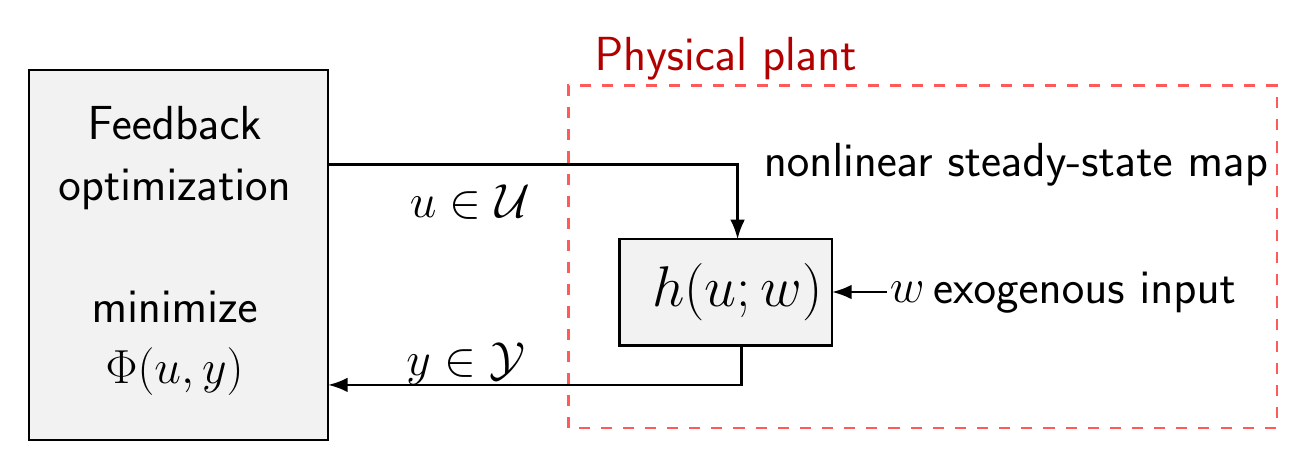
\begin{tikzpicture}[
    >=Latex,
    font=\sffamily,
    line width=0.9pt
]


% Left block
\draw[black, fill=gray!10] (-1.5,-2) rectangle (2.3,2.7);

\node[align=center, font=\sffamily\fontsize{19}{22}\selectfont] at (0.35,0.40) {Feedback\\optimization\\ \\minimize\\$\Phi(u,y)$};
%\node[align=center, font=\sffamily\fontsize{19}{22}\selectfont] at (1.35,-1.05) {minimize\\$\Phi(u,y)$};

% Red dashed plant box
\draw[red!65, dashed, line width=0.9pt, dash pattern=on 4pt off 4pt]
    (5.35,-1.85) rectangle (14.35,2.5);

% Plant title
\node[anchor=west, text=red!70!black, font=\sffamily\fontsize{18}{20}\selectfont]
    at (5.55,2.85) {Physical plant};

% Inner title
\node[anchor=west, font=\sffamily\fontsize{17}{20}\selectfont]
    at (7.7,1.50) {nonlinear steady-state map};

% Inner h block
\draw[black, fill=gray!10] (6,-0.80) rectangle (8.7,0.55);
\node[font=\fontsize{21}{24}\selectfont] at (7.50,-0.12) {$h(u;w)$};

% Top input line
\draw[->] (2.3,1.5) -- (7.50,1.5) -- (7.50,0.55);

% Bottom output line
\draw[->] (7.55,-0.8) -- (7.55,-1.3) -- (6.55,-1.30) -- (2.3,-1.30);

% Disturbance arrow
\draw[->] (9.4,-0.12) -- (8.7,-0.12);

% Labels
\node[font=\sffamily\fontsize{18}{20}\selectfont] at (4.10,1.02) {$u\in\mathcal{U}$};
\node[font=\sffamily\fontsize{18}{20}\selectfont] at (4.05,-1.03) {$y\in\mathcal{Y}$};

\node[anchor=west, font=\sffamily\fontsize{18}{20}\selectfont] at (9.30,-0.12) {$w$};
\node[anchor=west, font=\sffamily\fontsize{18}{20}\selectfont] at (9.85,-0.12) {exogenous input};

\end{tikzpicture}
    \caption{Certainty-equivalence view of steady-state optimization. The optimizer computes the input $u \in \mathcal U$ using the steady-state relation $y = h(u;w)$ so as to minimize the performance index $\Phi(u,y)$ while satisfying the steady-state constraints $y \in \mathcal Y$.}
    \label{fig:certainty-equivalence}
\end{figure}
This formulation expresses exactly the control objective discussed above: choose the input $u$ so that the plant settles at a feasible steady state $y$, while optimizing the desired economic or operational criterion.\\

If the exogenous quantity $w$ were known and the map $h$ were exactly available, then one could eliminate the variable $y$ and solve the reduced problem
\[
u^\star = \arg\min_{u \in \mathcal U} \tilde \Phi(u)
\qquad
\text{with}
\qquad
\tilde \Phi(u) := \Phi\bigl(u,h(u;w)\bigr),
\]
subject to
\[
h(u;w) \in \mathcal Y.
\]
Once the optimizer $u^\star$ has been computed, one simply applies it to the plant. This is the standard \emph{certainty-equivalence} or \emph{feedforward} approach: one behaves as if the uncertain quantities were known with certainty and as if the plant steady-state model were exact.\\

Conceptually, this is appealing because it reduces the problem to a classical nonlinear optimization task. However, this approach has two important weaknesses.\\
First, it requires accurate knowledge of the exogenous input $w$. In practice, $w$ may represent an unknown disturbance, a slowly varying demand, or an uncertain operating condition. If the value used in the optimization differs from the true one, then the computed input $u^\star$ is generally not the true optimizer for the physical plant. As a consequence, the achieved steady state may be suboptimal or may even violate the output constraints.\\

Second, the approach requires an accurate steady-state model $h$. If the map used in the optimization does not match the actual plant steady-state relation, then the predicted output
\[
y = h(u;w)
\]
is not the one that will actually be produced by the plant. Hence, even when the optimization problem is solved exactly, the resulting input may fail to achieve the desired steady-state specifications on the real system.\\

So the usual feedforward problem is clear: solving the static optimization problem is not enough when the disturbance is uncertain and the model is imperfect. The optimizer is optimal only for the \emph{model-based problem}, not necessarily for the physical plant. This is precisely the motivation for introducing feedback into the optimization loop.

A natural question then arises: \emph{how can we design feedback controllers that yield the desired autonomous closed-loop behavior?} The idea developed in feedback optimization is to combine two ingredients:
\begin{itemize}
    \item an algebraic input/output steady-state map
    \[
    y = h(u;w),
    \]
    valid when $w$ is constant or slowly changing;
    \item classical iterative nonlinear optimization algorithms.
\end{itemize}
Rather than solving the steady-state optimization problem once and applying the resulting input in open loop, we construct a controller that updates the input iteratively on the basis of measured plant outputs. In this way, the optimization algorithm and the physical plant become interconnected and the optimizer is embedded into the feedback loop. The resulting closed-loop system should drive the plant toward a steady state that satisfies the constraints and is optimal for the \emph{actual} plant, not only for the nominal model.

\subsubsection{Interconnecting plant and algorithms}

This viewpoint can be understood by comparing two different implementations.

In the first implementation, one keeps the optimization algorithm and the plant separate. The algorithm interacts only with a model of the steady-state map and solves
\[
\begin{aligned}
\min_{u,y}\quad & \Phi(u,y)\\
\text{s.t.}\quad & y \in \mathcal Y,\\
& u \in \mathcal U,\\
& y = h(u;w).
\end{aligned}
\]
The model returns the optimizer $u^\star$, and this value is then applied to the plant.
\begin{figure}[!h]
    \centering
    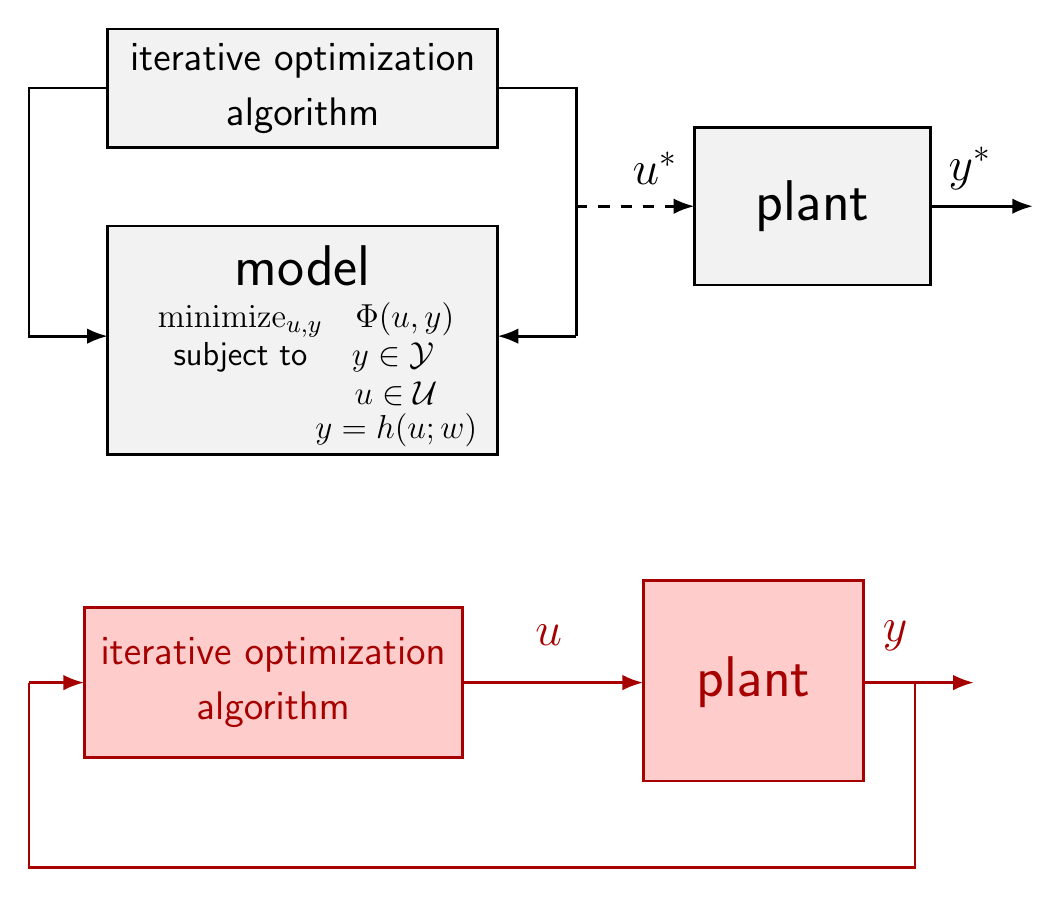
\begin{tikzpicture}[
    >=Latex,
    line width=1pt,
    font=\sffamily
]

% =========================================================
% TOP DIAGRAM
% =========================================================

% --- Top block: iterative optimization algorithm
\draw[fill=gray!10] (1.0,1.15) rectangle (5.95,2.65);
\node[align=center, font=\sffamily\fontsize{15}{20}\selectfont] at (3.475,1.90)
{iterative optimization\\algorithm};

% --- Bottom block: model
\draw[fill=gray!10] (1.0,-2.75) rectangle (5.95,0.15);

\node[font=\sffamily\fontsize{21}{24}\selectfont] at (3.475,-0.35) {model};

\node[anchor=west, font=\sffamily\fontsize{13}{16}\selectfont] at (1.50,-1.05)
{$\mathrm{minimize}_{u,y}\quad \Phi(u,y)$};

\node[anchor=west, font=\sffamily\fontsize{13}{16}\selectfont] at (1.70,-1.52)
{subject to \hspace{0.7em} $y\in\mathcal{Y}$};

\node[anchor=west, font=\sffamily\fontsize{13}{16}\selectfont] at (4,-1.98)
{$u\in\mathcal{U}$};

\node[anchor=west, font=\sffamily\fontsize{13}{16}\selectfont] at (3.5,-2.45)
{$y=h(u;w)$};

% --- Plant block
\draw[fill=gray!10] (8.45,-0.60) rectangle (11.45,1.40);
\node[font=\sffamily\fontsize{21}{24}\selectfont] at (9.95,0.40) {plant};

% --- Left feedback connection
\draw[->] (1.0,1.90) -- (0.0,1.90) -- (0.0,-1.25) -- (1.0,-1.25);

% --- Right connection from algorithm/model to plant
\draw[-] (5.95,1.90) -- (6.95,1.90) -- (6.95,-1.25);
\draw[->] (6.95,-1.25) -- (5.95,-1.25);

% dashed branch to plant
\draw[->, dashed, dash pattern=on 4pt off 4pt] (6.95,0.40) -- (8.45,0.40);

% --- Plant output
\draw[->] (11.45,0.40) -- (12.75,0.40);

% --- Labels
\node[font=\sffamily\fontsize{18}{20}\selectfont] at (7.95,0.88) {$u^{*}$};
\node[font=\sffamily\fontsize{18}{20}\selectfont] at (11.95,0.88) {$y^{*}$};

% =========================================================
% BOTTOM DIAGRAM
% =========================================================

\begin{scope}[yshift=-7.0cm, draw=red!65!black, text=red!65!black]

% blocks
\draw[fill=red!20] (0.7,0.4) rectangle (5.5,2.3);
\node[align=center, font=\sffamily\fontsize{14}{20}\selectfont] at (3.1,1.35)
{iterative optimization\\algorithm};

\draw[fill=red!20] (7.8,0.1) rectangle (10.6,2.65);
\node[font=\sffamily\fontsize{20}{24}\selectfont] at (9.2,1.35) {plant};

% forward path
\draw[->] (5.5,1.35) -- (7.8,1.35);
\draw[->] (10.6,1.35) -- (12.0,1.35);

% feedback loop
\draw[-] (11.25,1.35) -- (11.25,-1.0) -- (0.0,-1.0) -- (0.0,1.35);
\draw[->] (0.0,1.35) -- (0.7,1.35);

% labels
\node[font=\sffamily\fontsize{18}{20}\selectfont] at (6.6,1.95) {$u$};
\node[font=\sffamily\fontsize{18}{20}\selectfont] at (11.0,1.95) {$y$};

\end{scope}

\end{tikzpicture}
    \caption{Comparison between model-based feedforward optimization and feedback optimization. In the upper scheme, the iterative optimization algorithm is closed around the model and produces the command $u^\star$ that is then sent to the plant. In the lower scheme, the optimization algorithm is directly interconnected with the physical plant through the measured output $y$, thereby forming an autonomous feedback loop.}
    \label{fig:interconnection-optimization-plant}
\end{figure}
This is exactly the feedforward architecture discussed above. Its weakness is that the optimization loop closes around the \emph{model}, while the real plant appears only at the end, as a system to which the precomputed command is sent. Therefore, any mismatch between model and plant directly affects the achieved performance.

The alternative is to interconnect the optimization algorithm with the physical plant itself. In this case, the algorithm produces an input $u$, the plant responds with an output $y$, and this measured output is fed back to the algorithm. The optimization method is no longer driven only by a nominal model prediction, but by the actual plant behavior. As a consequence, the closed-loop system formed by
\[
\text{optimization algorithm} + \text{plant}
\]
becomes the main object of analysis and design.\\

This is the key conceptual step of feedback optimization. The optimization algorithm is no longer viewed as an offline numerical routine that computes a set-point. Instead, it is implemented dynamically and interconnected with the plant in feedback. The plant acts as part of the optimization loop, and the measured output provides the information needed to compensate unknown disturbances and model mismatch.\\

In summary, the transition is the following:
\begin{itemize}
    \item in feedforward optimization, the algorithm solves the steady-state problem on a model and sends the resulting optimizer to the plant;
    \item in feedback optimization, the algorithm is directly interconnected with the plant, and the plant measurements are used online to steer the iterative process toward the desired optimum.
\end{itemize}

This interconnection is what allows one to move beyond certainty-equivalence design and obtain an autonomous closed-loop behavior with improved robustness to uncertainty in $w$ and in the steady-state map $h$.\\

\subsubsection{Online feedback optimization}

The previous discussion motivates a shift from static feedforward optimization to \emph{online feedback optimization}. The idea is to implement an optimization algorithm as a dynamical system interacting directly with the plant, so that the plant measurements continuously correct the optimization process. In this way, the input is not computed once and for all from an uncertain model, but is updated online on the basis of the actual closed-loop behavior.\\

The steady-state optimization problem of interest is
\[
\begin{aligned}
\min_{u,y}\quad & \Phi(u,y)\\
\text{s.t.}\quad & y \in \mathcal Y,\\
& u \in \mathcal U,\\
& y = h(u;w).
\end{aligned}
\]
Using the steady-state relation, this problem can be equivalently written only in terms of the decision variable $u$ as
\[
\begin{aligned}
\min_{u \in \mathcal U}\quad & \Phi\bigl(u,h(u;w)\bigr)\\
\text{s.t.}\quad & h(u;w) \in \mathcal Y.
\end{aligned}
\]
So the plant enters the optimization problem through the algebraic steady-state map $y=h(u;w)$, while the constraints may act both directly on the input and indirectly on the output.\\

Once the problem has been written in this form, many classical iterative methods become available. In particular, the most relevant class for feedback optimization is that of \emph{first-order optimization algorithms}, that is, methods based on gradient information or generalized descent directions. Typical examples are:
\begin{itemize}
    \item gradient descent combined with penalty or barrier terms;
    \item projected gradient methods;
    \item primal--dual dynamics or primal--dual flows.
\end{itemize}
The reason these methods are attractive is that they admit iterative implementations that can naturally be interconnected with the plant. Instead of solving the optimization problem to completion at each step, one performs repeated correction steps, and the plant output provides the information needed to drive the iterations toward the desired optimum.

\subsection{First-order methods for feedback optimization}
\subsubsection{First-order optimization algorithms}

Let us now look more closely at the class of first-order methods. Consider again the constrained steady-state problem
\[
\begin{aligned}
\min_{u,y}\quad & \Phi(u,y)\\
\text{s.t.}\quad & y \in \mathcal Y,\\
& u \in \mathcal U,\\
& y = h(u;w).
\end{aligned}
\]
Equivalently, after eliminating $y$ through the steady-state map, we obtain
\[
\begin{aligned}
\min_{u \in \mathcal U}\quad & \Phi\bigl(u,h(u;w)\bigr)\\
\text{s.t.}\quad & h(u;w) \in \mathcal Y.
\end{aligned}
\]
This equivalent formulation is useful because it shows that the optimization variable can be taken to be only $u$, while the output constraint is enforced through the plant steady-state relation.\\

At this point, the problem has the structure of a nonlinear constrained optimization problem, and one may attack it with standard first-order techniques. The main issue is how to handle the constraints. A first possibility is to absorb the output constraint into the cost by adding a suitable extra term. This leads to gradient methods with \emph{penalty} or \emph{barrier} functions.

\subsubsection{Gradient descent with penalty / barrier}

Consider the constrained problem
\[
\begin{aligned}
\min_{u,y}\quad & \Phi(u,y)\\
\text{s.t.}\quad & y \in \mathcal Y,\\
& u \in \mathcal U,\\
& y = h(u;w).
\end{aligned}
\]
We focus here on the output constraint $y \in \mathcal Y$. A standard way to handle it is to transform the constrained problem into an unconstrained or less constrained one by modifying the cost function. Two classical constructions are the penalty approach and the barrier approach.

\paragraph{Penalty function.}
In the penalty approach, one introduces an additional term $p(y)$ in the objective and solves
\[
\min_{u,y} \; \Phi(u,y) + p(y).
\]
The function $p(y)$ is chosen so that it is small or zero when the constraint is satisfied, and increases when the output violates the admissible set $\mathcal Y$. In this way, constraint violations are discouraged, but not made impossible. Small violations may still occur if they lead to a lower total cost.\\

This approach is often attractive because it leads to a smooth unconstrained optimization problem, which is easy to handle with gradient-based methods. However, the price to pay is that feasibility is not enforced exactly: one only penalizes infeasibility. Therefore, the obtained solution may slightly violate the constraint, depending on the shape and weight of the penalty.

\begin{figure}[!h]
    \centering
    \begin{subfigure}{0.45\textwidth}
        \centering
        %==================================================
% First graph: p(y)
%==================================================
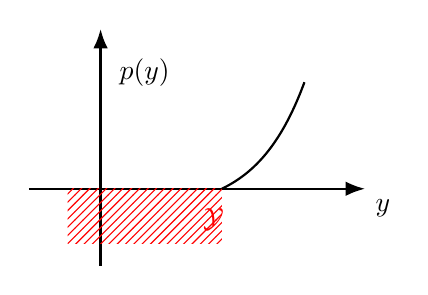
\begin{tikzpicture}[>=Latex, line width=0.9pt, scale=0.7]

% axes
\draw[->] (0,-1.4) -- (0,2.9);
\draw[->] (-1.3,0) -- (4.8,0) node[below right] {$y$};

% red shaded admissible set
\fill[pattern=north east lines, pattern color=red] (-0.6,-1.0) rectangle (2.2,0);

% labels
\node at (0.8,2.1) {$p(y)$};
\node[red] at (2.05,-0.55) {$\mathcal{Y}$};

% curve
\draw[thick, domain=2.2:3.7, samples=100, smooth]
  plot (\x,{0.42*(exp(1.15*(\x-2.2))-1)});

\end{tikzpicture}


        \caption{Penalty function.}
    \end{subfigure}
    \hfill
    \begin{subfigure}{0.45\textwidth}
        \centering
        %==================================================
% Second graph: b(y)
%==================================================
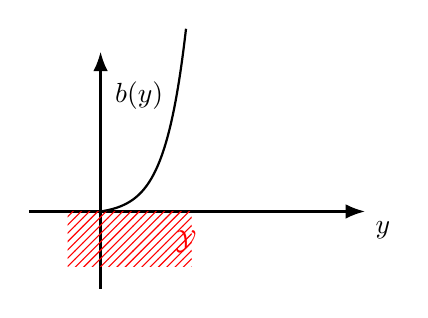
\begin{tikzpicture}[>=Latex, line width=0.9pt, scale=0.7]

% axes
\draw[->] (0,-1.4) -- (0,2.9);
\draw[->] (-1.3,0) -- (4.8,0) node[below right] {$y$};

% red shaded admissible set
\fill[pattern=north east lines, pattern color=red] (-0.6,-1.0) rectangle (1.65,0);

% labels
\node at (0.7,2.1) {$b(y)$};
\node[red] at (1.55,-0.55) {$\mathcal{Y}$};

% curve
\draw[thick, domain=0.0:1.55, samples=100, smooth]
  plot (\x,{0.06*(exp(2.6*\x)-1)});

\end{tikzpicture}
        \caption{Barrier function.}
    \end{subfigure}
    \caption{Qualitative comparison between penalty and barrier functions used to enforce the output constraint $y \in \mathcal Y$. A penalty function remains finite outside the feasible set and discourages violations without excluding them completely. A barrier function instead becomes unbounded at the boundary of the feasible set and is undefined outside it, thereby forcing the iterates to remain strictly feasible.}
    \label{fig:penalty-barrier}
\end{figure}

\paragraph{Barrier function.}
In the barrier approach, one instead introduces a function $b(y)$ and solves
\[
\min_{u,y} \; \Phi(u,y) + b(y).
\]
Now the function $b(y)$ is defined only inside the feasible set and tends to $+\infty$ as $y$ approaches the boundary of $\mathcal Y$. As a consequence, the optimizer is forced to remain in the interior of the feasible region.\\

This gives a more conservative behavior than the penalty approach. Since the barrier becomes very large near the boundary, the algorithm tends to stay away from it. Moreover, the formulation is not even defined outside the feasible set, so one must initialize and operate the algorithm inside the admissible region. The benefit is that feasibility is preserved by construction, at least in the ideal continuous-time or exact-iteration picture.

\paragraph{Comparison.}
The two approaches reflect two different ways of dealing with constraints:
\begin{itemize}
    \item with a \emph{penalty function}, small violations are acceptable, since infeasibility is merely discouraged;
    \item with a \emph{barrier function}, one is conservative and never reaches the boundary, because leaving the feasible region is forbidden by the formulation itself.
\end{itemize}

These ideas are particularly useful in feedback optimization because they turn constrained optimization into a form that can be handled by simple first-order iterative laws. The optimization algorithm then updates the input $u$ by descending along the modified objective, while the plant provides the output $y$ entering the cost and the constraint-handling terms.

\subsubsection{Unconstrained gradient descent}

Before applying gradient methods to the feedback optimization problem, it is useful to recall the basic convergence property of gradient descent in the unconstrained case. Consider the problem
\[
\min_x \; \phi(x),
\]
and assume that $\phi$ is twice continuously differentiable and has bounded second derivative, namely
\[
\nabla^2 \phi(x) \preceq MI
\qquad \forall x,
\]
for some constant $M>0$. This means that the gradient of $\phi$ is Lipschitz continuous with Lipschitz constant bounded by $M$.\\
The gradient descent iteration is
\[
x_{k+1}=x_k-\alpha \nabla \phi(x_k),
\]
where $\alpha>0$ is the stepsize. Under the assumption above, this iteration converges to a local minimum of $\phi$ provided that
\[
\alpha < \frac{2}{M}.
\]
The reason is seen by expanding $\phi$ around the current iterate $x_k$. By Taylor's formula,
\[
\phi(x_{k+1})
=
\phi(x_k)
+
\nabla \phi(x_k)^\top (x_{k+1}-x_k)
+
\frac{1}{2}(x_{k+1}-x_k)^\top \nabla^2\phi(z)(x_{k+1}-x_k),
\]
where $z$ is a point on the segment joining $x_k$ and $x_{k+1}$. Substituting the gradient descent update
\[
x_{k+1}-x_k=-\alpha \nabla\phi(x_k),
\]
we obtain
\[
\phi(x_{k+1})
=
\phi(x_k)
-\alpha \|\nabla\phi(x_k)\|^2
+
\frac{\alpha^2}{2}\nabla\phi(x_k)^\top \nabla^2\phi(z)\nabla\phi(x_k).
\]
Using the bound $\nabla^2\phi(z)\preceq MI$, the last term can be bounded as
\[
\nabla\phi(x_k)^\top \nabla^2\phi(z)\nabla\phi(x_k)
\leq
M\|\nabla\phi(x_k)\|^2,
\]
and therefore
\[
\phi(x_{k+1})
\leq
\phi(x_k)
-\alpha \|\nabla\phi(x_k)\|^2
+
\frac{\alpha^2 M}{2}\|\nabla\phi(x_k)\|^2.
\]
Equivalently,
\[
\phi(x_{k+1})
\leq
\phi(x_k)
-\alpha\left(1-\frac{\alpha M}{2}\right)\|\nabla\phi(x_k)\|^2.
\]
Hence, if
\[
\alpha<\frac{2}{M},
\]
the coefficient in parentheses is positive, and so
\[
\phi(x_{k+1})<\phi(x_k)
\qquad \text{whenever } \nabla\phi(x_k)\neq 0.
\]
So the sequence $\phi(x_k)$ is decreasing along the iterations until the gradient vanishes. This is the key fact behind convergence of gradient descent: the cost decreases monotonically, and the iterates are driven toward the set of stationary points
\[
\{x:\nabla\phi(x)=0\}.
\]
Under suitable additional assumptions, this implies convergence to a local minimum.

\subsubsection{Gradient descent with penalty}

We now apply this idea to the steady-state optimization problem in the presence of output constraints handled through a penalty term. Starting from
\[
\begin{aligned}
\min_{u,y}\quad & \Phi(u,y)\\
\text{s.t.}\quad & y \in \mathcal Y,\\
& u \in \mathcal U,\\
& y = h(u;w),
\end{aligned}
\]
we incorporate the constraint $y\in\mathcal Y$ into the objective through a penalty function $p(y)$ and obtain the problem
\[
\min_{u\in\mathcal U} \; \Phi\bigl(u,h(u;w)\bigr) + p\bigl(h(u;w)\bigr).
\]
Here the admissible input set $\mathcal U$ is kept explicitly, while the output constraint is treated by penalization.\\
To derive a gradient algorithm, define the penalized objective
\[
J(u):=\Phi\bigl(u,h(u;w)\bigr)+p\bigl(h(u;w)\bigr).
\]
Then the gradient descent iteration is
\[
u_{k+1}=u_k-\alpha \nabla J(u_k).
\]
Using the chain rule, the gradient of $J$ is
\[
\nabla J(u)
=
\nabla_u \Phi(u,h(u;w))
+
\nabla_u h(u;w)^\top \nabla_y \Phi(u,h(u;w))
+
\nabla_u h(u;w)^\top \nabla_y p(h(u;w))
\].
Therefore, the gradient descent algorithm becomes
\[
u_{k+1}
=
u_k
-
\alpha\Bigl(
\nabla_u \Phi(u_k,\textcolor{red}{h(u_k;w)})
+
\nabla_u h(u_k;w)^\top \nabla_y \Phi(u_k,\textcolor{red}{h(u_k;w)})
+
\nabla_u h(u_k;w)^\top \nabla_y p(\textcolor{red}{h(u_k;w)})
\Bigr).
\]
This is the ideal algorithm one would write if the steady-state map $h$ were exactly known. However, in feedback optimization we do not want to evaluate the cost only on the basis of the model output $h(u_k;w)$; rather, we want to use the \emph{measured} plant output. Denoting by $\textcolor{red}{y_k}$ the measured output corresponding to the current input $u_k$, the update law becomes
\[
u_{k+1}
=
u_k
-
\alpha\Bigl(
\nabla_u \Phi(u_k,\textcolor{red}{y_k})
+
\nabla_u h(u_k;w)^\top \nabla_y \Phi(u_k,\textcolor{red}{y_k})
+
\nabla_u h(u_k;w)^\top \nabla_y p(\textcolor{red}{y_k})
\Bigr).
\]
This is the \emph{gradient descent controller}: the optimization step is corrected using the actual output measurement $y_k$, while the Jacobian $\nabla_u h(u_k;w)$ is still taken from the model. The input is finally constrained to lie in $\mathcal U$, for instance by saturation or projection.\\
The structure of the controller is worth interpreting carefully:
\begin{itemize}
    \item $\nabla_u \Phi(u_k,y_k)$ measures the direct effect of the input on the cost;
    \item $\nabla_y \Phi(u_k,y_k)$ measures how the cost changes with the output;
    \item $\nabla_y p(y_k)$ measures how strongly the penalty reacts to output constraint violations;
    \item $\nabla_u h(u_k;w)$ maps output sensitivities back to input directions.
\end{itemize}
So the matrix
\[
\nabla_u h(u;w)^\top
\]
plays a crucial role: it tells us how a change in input affects the steady-state output, and therefore how to translate output-based optimization information into an input update.

\paragraph{Steady-state sensitivities.}
The quantity
\[
\nabla_u h(u;w)^\top
\]
is the transpose of the Jacobian of the steady-state map with respect to the input. It is the local steady-state input--output sensitivity matrix. If the output dimension is $p$ and the input dimension is $m$, then
\[
\nabla_u h(u;w)\in\mathbb R^{p\times m},
\]
and its $(i,j)$-th entry is
\[
\frac{\partial h_i(u;w)}{\partial u_j}.
\]
This derivative tells us how the $i$-th steady-state output changes when the $j$-th input is perturbed.\\
For a linear fast-stable plant, where
\[
y=Hu+Lw,
\]
the steady-state sensitivity is simply constant:
\[
\nabla_u h(u;w)=H.
\]
So in the linear case the controller uses the steady-state gain matrix $H^\top$.\\

In nonlinear plants, instead, the sensitivity depends on the current operating point. Some intuitive examples are the following:
\begin{itemize}
    \item in a compressor or process unit, the derivative describes how the steady-state flow, pressure, or efficiency changes when a valve opening or actuator set-point is modified;
    \item in power systems, it represents how steady-state frequency, power flow, or voltage-related quantities react to a change in generation dispatch;
    \item in thermal systems, it measures how the equilibrium temperature changes when heater power or coolant flow is varied.
\end{itemize}
Thus, the Jacobian $\nabla_u h(u;w)$ is exactly the information needed to connect an optimization algorithm to the physical plant at steady state.\\

The key point is that the controller does not require a full dynamic model of the plant. It only needs a model, estimate, or approximation of the steady-state sensitivities. This is much weaker than full model-based control and is one of the main reasons why feedback optimization is attractive in applications where the transient dynamics are uncertain but the steady-state behavior is sufficiently structured.

\subsubsection{Projected gradient descent}

Penalty and barrier methods handle the output constraint indirectly by modifying the objective function. A different possibility is to enforce the constraints explicitly through projection. Starting from
\[
\begin{aligned}
\min_{u,y}\quad & \Phi(u,y)\\
\text{s.t.}\quad & y \in \mathcal Y,\\
& u \in \mathcal U,\\
& y = h(u;w),
\end{aligned}
\]
and eliminating the variable $y$ through the steady-state relation, we obtain
\[
\min_{u} \; \Phi\bigl(u,h(u;w)\bigr)
\]
subject to
\[
u \in \mathcal U,
\qquad
h(u;w)\in\mathcal Y.
\]
It is convenient to collect both feasibility requirements into a single admissible set for the input:
\[
\tilde{\mathcal U}:=\mathcal U \cap h^{-1}(\mathcal Y;w),
\]
where
\[
h^{-1}(\mathcal Y;w)
:=
\{u:\; h(u;w)\in\mathcal Y\}.
\]
Then the optimization problem can be rewritten as
\[
\min_{u\in\tilde{\mathcal U}} \; \Phi\bigl(u,h(u;w)\bigr).
\]
This suggests the use of projected gradient descent: one first takes a descent step for the cost, and then projects the result back onto the feasible set $\tilde{\mathcal U}$. Formally, if
\[
J(u):=\Phi\bigl(u,h(u;w)\bigr),
\]
the projected gradient iteration is
\[
u_{k+1}
=
\Pi_{\tilde{\mathcal U}}
\Bigl(
u_k-\alpha \nabla J(u_k)
\Bigr),
\]
where $\Pi_{\tilde{\mathcal U}}$ denotes the Euclidean projection onto $\tilde{\mathcal U}$.\\
The appealing feature of this method is that, unlike a penalty formulation, it tries to maintain feasibility explicitly. The difficulty, however, is hidden in the projection step. While projection onto the input set $\mathcal U$ may be easy, the set
\[
h^{-1}(\mathcal Y;w)
\]
is generally complicated. Even when $\mathcal Y$ is a simple set, its inverse image through a nonlinear steady-state map may be highly nonconvex and may have a complicated geometry. As a consequence, projecting onto
\[
\tilde{\mathcal U}=\mathcal U\cap h^{-1}(\mathcal Y;w)
\]
can be numerically difficult and conceptually unpleasant. This is exactly the issue highlighted by figure \ref{fig:inverse-image-geometry}: a simple admissible set in the output space may correspond, in the input space, to a distorted and difficult set.\\

To make this approach practical, one would like a good approximation of the set $h^{-1}(\mathcal Y;w)$ that satisfies two properties:
\begin{itemize}
    \item it should be easy to project onto, ideally a polytope or another simple convex set;
    \item it should be sufficiently accurate, especially near the boundary of $\mathcal Y$, where constraint satisfaction matters most.
\end{itemize}

A common assumption is that the admissible sets are polyhedral:
\[
\mathcal U:=\{u\in\mathbb R^m:\; Au\leq b\},
\qquad
\mathcal Y:=\{y\in\mathbb R^p:\; Cy\leq d\}.
\]
In this case, the difficulty is entirely due to the nonlinear steady-state map. The set $\mathcal Y$ is simple in the output space, but its inverse image through $h$ is not.

\begin{figure}[!h]
    \centering
    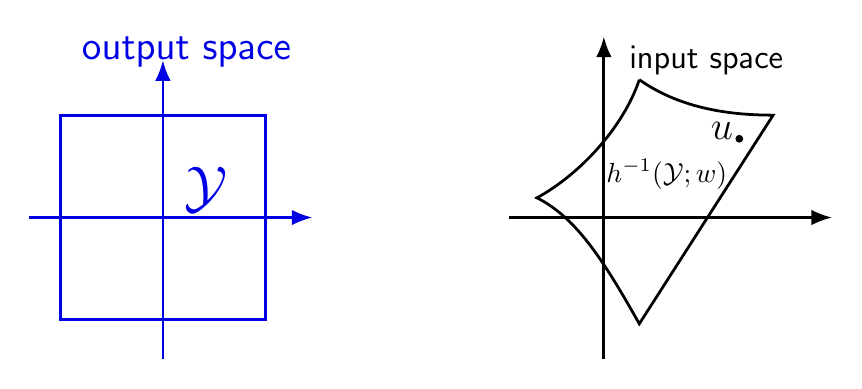
\begin{tikzpicture}[
    >=Latex,
    line width=1pt,
    font=\sffamily
]

% =========================================================
% LEFT: output space
% =========================================================
\begin{scope}[xshift=0cm, yshift=0cm, draw=blue!90!black, text=blue!90!black]

% axes
\draw[->] (-1.7,0) -- (1.9,0);
\draw[->] (0,-1.8) -- (0,2.0);

% square
\draw (-1.3,-1.3) rectangle (1.3,1.3);

% labels
\node[font=\sffamily\fontsize{14}{16}\selectfont] at (0.3,2.1) {output space};
\node[font=\fontsize{20}{22}\selectfont] at (0.55,0.35) {$\mathcal{Y}$};

\end{scope}

% =========================================================
% MIDDLE: input space and preimage
% =========================================================
\begin{scope}[xshift=5.6cm, yshift=0cm, draw=black, text=black]

% axes
\draw[->] (-1.2,0) -- (2.9,0);
\draw[->] (0,-1.8) -- (0,2.3);

% feasible set shape
\draw
    (0.45,1.75)
    .. controls (0.25,1.15) and (-0.30,0.55) .. (-0.85,0.25)
    .. controls (-0.35,0.00) and (0.00,-0.55) .. (0.45,-1.35)
    -- (2.15,1.30)
    .. controls (1.55,1.30) and (0.95,1.40) .. (0.45,1.75);

% point and labels
\fill (1.72,1.0) circle (1.4pt);
\node[font=\fontsize{15}{17}\selectfont] at (1.5,1.10) {$u$};
\node[font=\fontsize{10}{22}\selectfont] at (0.8,0.55) {$h^{-1}(\mathcal{Y};w)$};

% labels
\node[font=\sffamily\fontsize{12}{16}\selectfont] at (1.3,2) {input space};

\end{scope}



\end{tikzpicture}
    \caption{Geometry of the output constraint and its inverse image in the input space. A simple polyhedral constraint set $\mathcal Y$ in the output space induces, through the nonlinear map $h(u;w)$, a generally complicated feasible region $h^{-1}(\mathcal Y;w)$ in the input space. Intersecting this set with the input constraint set $\mathcal U$ yields the feasible set for projected gradient descent.}
    \label{fig:inverse-image-geometry}
\end{figure}

The natural way to obtain a tractable approximation is to linearize the steady-state map around the current input $u$. Using a first-order Taylor expansion, for a nearby point $u'$ we have
\[
h(u';w)\approx h(u;w)+\nabla_u h(u;w)^\top (u'-u).
\]
If the output constraint is
\[
Cy\leq d,
\]
then substituting the first-order approximation gives
\[
C\,h(u';w)\leq d
\quad\Rightarrow\quad
C\Bigl(h(u;w)+\nabla_u h(u;w)^\top (u'-u)\Bigr)\leq d.
\]
This defines a local first-order approximation of the inverse image $h^{-1}(\mathcal Y;w)$ around the current point $u$. Importantly, this approximation is affine in $u'$, and therefore it produces a polyhedral local approximation of the feasible set in the input space.

So, instead of projecting onto the exact set $h^{-1}(\mathcal Y;w)$, which is difficult, one projects onto its linearized approximation. This preserves the main advantage of projected methods, namely explicit constraint handling, while replacing the hard nonlinear projection with a much simpler projection onto a local polytope.

\begin{figure}[!h]
    \centering
    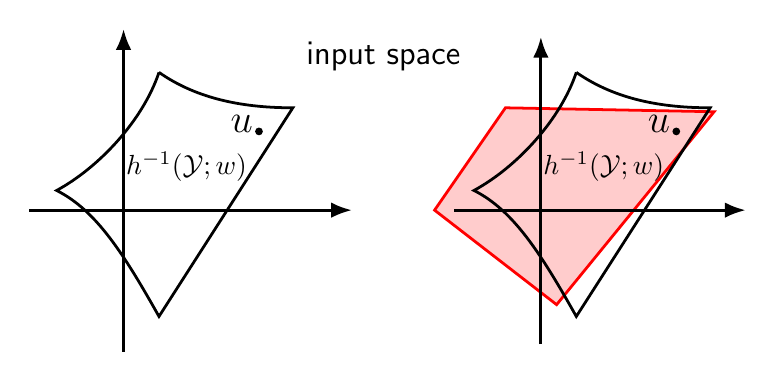
\begin{tikzpicture}[
    >=Latex,
    line width=1pt,
    font=\sffamily
]


% =========================================================
% MIDDLE: input space and preimage
% =========================================================
\begin{scope}[xshift=5.6cm, yshift=0cm, draw=black, text=black]

% axes
\draw[->] (-1.2,0) -- (2.9,0);
\draw[->] (0,-1.8) -- (0,2.3);

% feasible set shape
\draw
    (0.45,1.75)
    .. controls (0.25,1.15) and (-0.30,0.55) .. (-0.85,0.25)
    .. controls (-0.35,0.00) and (0.00,-0.55) .. (0.45,-1.35)
    -- (2.15,1.30)
    .. controls (1.55,1.30) and (0.95,1.40) .. (0.45,1.75);

% point and labels
\fill (1.72,1.0) circle (1.4pt);
\node[font=\fontsize{15}{17}\selectfont] at (1.5,1.10) {$u$};
\node[font=\fontsize{10}{22}\selectfont] at (0.8,0.55) {$h^{-1}(\mathcal{Y};w)$};

\end{scope}

% =========================================================
% RIGHT: input space with red highlighted region
% =========================================================
\begin{scope}[xshift=10.9cm, yshift=0cm]

% red highlighted polygon
\filldraw[fill=red!20, draw=red, line width=1pt]
    (-0.45,1.30) --
    (2.2,1.25) --
    (0.2,-1.20) --
    (-1.35,0.00) -- cycle;

% axes
\draw[->] (-1.1,0) -- (2.6,0);
\draw[->] (0,-1.7) -- (0,2.2);

% feasible set shape
\draw
    (0.45,1.75)
    .. controls (0.25,1.15) and (-0.30,0.55) .. (-0.85,0.25)
    .. controls (-0.35,0.00) and (0.00,-0.55) .. (0.45,-1.35)
    -- (2.15,1.30)
    .. controls (1.55,1.30) and (0.95,1.40) .. (0.45,1.75);

% point and labels
\fill (1.72,1.0) circle (1.4pt);
\node[font=\fontsize{15}{17}\selectfont] at (1.5,1.10) {$u$};
\node[font=\fontsize{10}{22}\selectfont] at (0.8,0.55) {$h^{-1}(\mathcal{Y};w)$};

% labels
\node[font=\sffamily\fontsize{12}{16}\selectfont] at (-2,1.95) {input space};

\end{scope}

\end{tikzpicture}
    \caption{First-order approximation of the inverse image of the output constraint. Linearizing the steady-state map around the current input $u$ transforms the nonlinear feasible set $h^{-1}(\mathcal Y;w)$ into a local polyhedral approximation that is much easier to use in a projection step.}
    \label{fig:inverse-image-linearization}
\end{figure}

This leads to the following interpretation. Projected gradient descent is conceptually attractive, because it tries to enforce feasibility directly. However, the exact feasible set in the input space is usually too complicated. The practical solution is therefore to replace the exact inverse image of the output constraints with a local first-order approximation based on the steady-state sensitivities
\[
\nabla_u h(u;w).
\]
Once again, the steady-state Jacobian is the central object: it provides the linear map that translates output constraints into approximate input constraints.

In summary:
\begin{itemize}
    \item the exact projected method would require projection onto
    \[
    \tilde{\mathcal U}=\mathcal U\cap h^{-1}(\mathcal Y;w),
    \]
    which is generally difficult;
    \item if $\mathcal U$ and $\mathcal Y$ are polyhedral, then a local linearization of $h$ gives a polyhedral approximation of $h^{-1}(\mathcal Y;w)$;
    \item this approximation makes projection computationally tractable and connects projected methods again to the steady-state sensitivity matrix $\nabla_u h(u;w)$.
\end{itemize}

\subsubsection{Projected gradient flow via repeated quadratic programming}

The discussion above suggests a practical refinement of projected gradient descent. The exact projection onto
\[
\tilde{\mathcal U}=\mathcal U\cap h^{-1}(\mathcal Y;w)
\]
is typically hard, because the inverse image of the output constraint through the nonlinear steady-state map is not easy to describe explicitly. However, once a local first-order approximation of this inverse image is available, the projection step can be replaced by the solution of a simple quadratic program.

Assume that the input and output constraint sets are polyhedral:
\[
\mathcal U:=\{u\in\mathbb R^m:Au\le b\},
\qquad
\mathcal Y:=\{y\in\mathbb R^p:Cy\le d\}.
\]
As seen above, around the current operating point $u$ we can approximate the output constraint through the linearization
\[
h(u';w)\approx h(u;w)+\nabla_u h(u;w)^\top (u'-u).
\]
Therefore, the condition $y\in\mathcal Y$, namely
\[
Cy\le d,
\]
is locally approximated by
\[
C\Bigl(h(u;w)+\nabla_u h(u;w)^\top (u'-u)\Bigr)\le d.
\]

This suggests the following idea. Instead of computing the exact Euclidean projection of a gradient step onto the nonlinear feasible set, we search for a correction direction that is as close as possible to the negative gradient while satisfying the linearized input and output constraints. In this way, each projected step is obtained by solving a quadratic program.

Let
\[
g_k:=
\nabla_u \Phi(u_k,y_k)
+
\nabla_u h(u_k;w)^\top \nabla_y \Phi(u_k,y_k),
\]
where $y_k$ is the measured steady-state output corresponding to the current input $u_k$. The vector $-g_k$ is the descent direction that would be used in the unconstrained gradient method. Since constraints are present, we cannot move arbitrarily along this direction. We therefore compute a feasible correction $\delta u_k$ as the solution of the quadratic program
\[
\delta u_k
:=
\arg\min_{v}\;
\left\|
v-(-g_k)
\right\|^2
\]
subject to
\[
A(u_k+\alpha v)\le b,
\]
\[
C\Bigl(y_k+\alpha \nabla_u h(u_k;w)^\top v\Bigr)\le d.
\]
The input is then updated according to
\[
u_{k+1}=u_k+\alpha \delta u_k.
\]

This construction has a clear interpretation. The optimization variable $v$ is a candidate input increment. The quadratic objective forces $v$ to remain as close as possible to the nominal negative gradient direction. The first constraint
\[
A(u_k+\alpha v)\le b
\]
imposes that the next input remains in the admissible input set $\mathcal U$. The second constraint
\[
C\Bigl(y_k+\alpha \nabla_u h(u_k;w)^\top v\Bigr)\le d
\]
is a first-order approximation of the output feasibility condition, centered at the current measurement $y_k$. So the quadratic program computes the feasible direction that best approximates the desired descent step.

This is why one may speak of \emph{projected gradient flow via repeated quadratic programming}: the projection is no longer performed onto the exact nonlinear feasible set, but onto a local linearized approximation, and this approximate projection is obtained by solving a small QP at each iteration.

Several features of this construction are worth emphasizing.

First, the method uses the measured output $y_k$ rather than the predicted value $h(u_k;w)$ in the constraint linearization. This is consistent with the feedback optimization philosophy: the plant measurement corrects the optimization step online and helps compensate model mismatch in the steady-state map itself.

Second, the Jacobian
\[
\nabla_u h(u_k;w)
\]
again plays the central role. It provides the local map from input variations to output variations, and therefore determines how output constraints are translated into local linear constraints on the input increment.

Third, the quadratic program is simple. Its cost is quadratic and convex, and its constraints are affine. Hence, under standard regularity conditions, it can be solved efficiently and repeatedly online. This makes the method much more practical than exact projection onto the nonlinear set $\tilde{\mathcal U}$.

In summary, the repeated-QP construction provides a tractable approximation of projected gradient descent:
\begin{itemize}
    \item the unconstrained negative gradient gives the desired descent direction;
    \item the input and output constraints are enforced through local affine approximations;
    \item the feasible direction closest to the negative gradient is obtained from a quadratic program;
    \item the resulting update law preserves the feedback character of the method, because it is based on measured outputs and local steady-state sensitivities.
\end{itemize}

So the overall controller can be interpreted as a feedback optimization algorithm that repeatedly solves a local QP in order to generate a descent direction compatible with both input and output constraints.

\subsection{Duality-based methods}
\subsubsection{Dual problem}

Another important family of first-order methods for constrained optimization is based on \emph{duality}. The idea is to keep the constraints explicitly, but to move them into the objective through Lagrange multipliers. This leads naturally to primal--dual algorithms and dual ascent methods, which are particularly well suited to feedback optimization.

To explain the idea, consider first the generic constrained optimization problem
\[
\min_x \; \phi(x)
\qquad
\text{subject to}
\qquad
g(x)\le 0,
\]
where $g(x)\in\mathbb R^q$ collects the inequality constraints.

The associated Lagrangian is
\[
\mathcal L(x,\lambda):=\phi(x)+\lambda^\top g(x),
\]
where the multiplier vector satisfies
\[
\lambda\ge 0.
\]
The role of $\lambda$ is to penalize constraint violations: whenever some component of $g(x)$ is positive, the corresponding multiplier increases the Lagrangian cost.

Under suitable convexity assumptions and constraint qualifications, strong duality holds. In that case, the original constrained problem can be written equivalently as
\[
\min_{x:\, g(x)\le 0}\phi(x)
=
\min_x \max_{\lambda\ge 0}\mathcal L(x,\lambda)
=
\max_{\lambda\ge 0}\min_x \mathcal L(x,\lambda).
\]
This identity is the key reason why dual methods are useful: instead of solving the constrained problem directly, one may solve the saddle-point problem associated with the Lagrangian.

It is worth understanding the first equality. For a fixed $x$, consider
\[
\max_{\lambda\ge 0}\mathcal L(x,\lambda)
=
\max_{\lambda\ge 0}\bigl(\phi(x)+\lambda^\top g(x)\bigr).
\]
If $g(x)\le 0$, then the maximum is attained at $\lambda=0$, so
\[
\max_{\lambda\ge 0}\mathcal L(x,\lambda)=\phi(x).
\]
If instead some component of $g(x)$ is positive, then by increasing the corresponding multiplier one obtains
\[
\max_{\lambda\ge 0}\mathcal L(x,\lambda)=+\infty.
\]
So maximizing over the nonnegative multipliers has the effect of enforcing the constraint: infeasible points are assigned infinite cost, while feasible points retain their original objective value. In this sense, the Lagrangian reformulation replaces the constraint by an indicator-like mechanism.

This viewpoint is particularly useful in feedback optimization, because it leads to algorithms in which the primal variable performs a descent step, while the multiplier performs an ascent step. The multiplier then acts as an internal controller state that stores how strongly the output constraints are being violated.

\subsubsection{Primal--dual iterations}

The dual reformulation suggests natural iterative schemes for solving constrained optimization problems. Consider again the saddle-point problem
\[
\max_{\lambda\ge 0}\min_x \mathcal L(x,\lambda),
\qquad
\mathcal L(x,\lambda)=\phi(x)+\lambda^\top g(x).
\]
A first possibility is to apply gradient descent in the primal variable and gradient ascent in the dual variable. This yields the \emph{primal descent / dual ascent} iteration
\[
x_{k+1}=x_k-\alpha \nabla_x \mathcal L(x_k,\lambda_k),
\]
\[
\lambda_{k+1}=\lambda_k+\beta \nabla_\lambda \mathcal L(x_k,\lambda_k),
\]
followed, if needed, by projection of $\lambda_{k+1}$ onto the nonnegative orthant in order to preserve the condition $\lambda\ge 0$.

The logic is clear: one tries to decrease the Lagrangian with respect to the primal variable $x$, while increasing it with respect to the dual variable $\lambda$, since the saddle-point problem is a minimization in $x$ and a maximization in $\lambda$.

A second possibility is to minimize the Lagrangian exactly with respect to the primal variable at each step, and then update only the multiplier by ascent. This gives the \emph{dual ascent} scheme
\[
x_k=\arg\min_x \mathcal L(x,\lambda_k),
\]
\[
\lambda_{k+1}=\lambda_k+\beta \nabla_\lambda \mathcal L(x_k,\lambda_k).
\]
This method can be interpreted as a two-time-scale version of the primal--dual iteration: the primal variable reacts quickly and is assumed to be close to the minimizer of the current Lagrangian, while the multiplier evolves more slowly. In this sense, dual ascent is closely related to saddle-flow ideas with a slow dual dynamics.

A key observation is that
\[
\nabla_\lambda \mathcal L(x,\lambda)=g(x),
\]
because the Lagrangian is affine in the multiplier:
\[
\mathcal L(x,\lambda)=\phi(x)+\lambda^\top g(x).
\]
So the dual update is simply driven by the constraint violation. If the constraint is satisfied with margin, the multiplier tends not to grow; if the constraint is violated, the corresponding component of $\lambda$ increases. This is exactly the mechanism by which the multiplier enforces feasibility.

\subsubsection{Dual ascent for feedback optimization}

We now specialize the primal--dual idea to the steady-state optimization problem of feedback optimization. Suppose that the output constraint set can be written as
\[
\mathcal Y:=\{y\in\mathbb R^p:\; g(y)\le 0\},
\]
where $g(y)\in\mathbb R^q$ collects the inequality constraints on the steady-state output.

Starting from the steady-state optimization problem
\[
\min_{u,y}\; \Phi(u,y)
\qquad
\text{subject to}
\qquad
u\in\mathcal U,\quad y=h(u;w),\quad g(y)\le 0,
\]
we form the Lagrangian
\[
\mathcal L(u,\lambda)
:=
\Phi\bigl(u,h(u;w)\bigr)+\lambda^\top g\bigl(h(u;w)\bigr),
\]
with
\[
\lambda\ge 0.
\]
Here the multiplier is associated with the output constraints. It increases the cost whenever the measured or predicted output violates the admissible set.

Applying the primal descent / dual ascent idea gives an iterative controller. The primal variable is the input $u$, while the dual variable is the multiplier $\lambda$. Using measurements for the output and a model only for the steady-state sensitivities, one obtains the update
\[
u_{k+1}
=
u_k
-
\alpha\Bigl(
\nabla_u \Phi(u_k,y_k)
+
\nabla_u h(u_k;w)^\top \nabla_y \Phi(u_k,y_k)
+
\textcolor{red}{\nabla_u h(u_k;w)^\top \nabla g(y_k)^\top \lambda_k}
\Bigr),
\]
and
\[
\lambda_{k+1}
=
\Pi_{\ge 0}\bigl[\lambda_k+\beta g(y_k)\bigr].
\]
Here:
\begin{itemize}
    \item $y_k$ is the measured plant output at iteration $k$;
    \item $\nabla_u h(u_k;w)$ is the steady-state sensitivity matrix provided by the model;
    \item $\Pi_{\ge 0}$ denotes projection onto the nonnegative orthant.
\end{itemize}

The interpretation of these equations is very important.

The primal update for $u_k$ has the same structure as the gradient-based controllers discussed before, but now there is an \textcolor{red}{extra term},
\[
\nabla_u h(u_k;w)^\top \nabla g(y_k)^\top \lambda_k,
\]
which comes from the Lagrange multiplier. This term pushes the input in a direction that reduces constraint violations. The stronger the current multiplier $\lambda_k$, the stronger the correction induced by the constraint.

The dual update is even more intuitive:
\[
\lambda_{k+1}
=
\Pi_{\ge 0}\bigl[\lambda_k+\beta g(y_k)\bigr].
\]
If some constraint is violated, then the corresponding component of $g(y_k)$ is positive, and so the corresponding multiplier increases. If instead the constraint is satisfied, the multiplier does not need to grow. The projection ensures that the multipliers remain nonnegative, as required by duality theory.

Once again, the implementation is remarkably light in terms of modeling requirements. The controller does not need a full dynamic model of the plant. It only needs:
\begin{itemize}
    \item measurements of the current steady-state output $y_k$;
    \item the steady-state sensitivity matrix $\nabla_u h(u_k;w)$.
\end{itemize}
This is fully consistent with the feedback optimization philosophy developed so far.

\paragraph{Role of the multiplier as controller memory.}
An important conceptual question is: what is the role of the internal variable $\lambda_k$? The answer is that $\lambda_k$ provides \emph{memory} to the controller.

In plain gradient descent, the input update depends only on the current measurement and the current gradient information. In primal--dual control, instead, the multiplier stores information about past constraint violations. If a constraint has been active or violated for several iterations, the corresponding multiplier grows and keeps influencing the future control actions. In this sense, $\lambda_k$ acts as an internal state that accumulates constraint-related information over time.

This is closely analogous to integral action in regulation problems. Just as an integral state accumulates tracking error in order to remove steady-state offset, the multiplier accumulates constraint violation in order to enforce feasibility. For this reason, the dual variable can be interpreted as a memory state of the feedback optimizer, dedicated specifically to the handling of output constraints.

So the primal--dual controller has a clear structure:
\begin{itemize}
    \item the primal variable $u_k$ moves in a descent direction for performance optimization;
    \item the dual variable $\lambda_k$ integrates constraint violations;
    \item the interaction between the two produces a feedback law that seeks both optimality and feasibility.
\end{itemize}

This makes dual ascent and primal--dual iterations a very natural tool for online feedback optimization with constrained steady-state outputs.

\subsubsection{An old friend: dual ascent and PI control}

The primal--dual viewpoint is not only a mathematical construction. In an important special case, it recovers a very classical feedback controller.

Consider the linear steady-state relation
\[
y=Hu+w,
\]
where $u$ is the manipulated input, $y$ is the steady-state output, $w$ is a constant exogenous signal, and $r$ is the desired reference. Suppose we want to track the reference while keeping the input effort small. A natural optimization problem is
\[
\begin{aligned}
\min_{u,y}\quad & \frac{1}{2}\|u\|^2+\frac{\rho}{2}\|Hu+w-r\|^2\\
\text{s.t.}\quad & y=r,\\
& y=Hu+w.
\end{aligned}
\]
Equivalently, the constraint $y=r$ imposes exact tracking, while the term weighted by $\rho$ plays the role of an augmented penalty on the steady-state mismatch. This is an augmented-Lagrangian formulation of the regulation problem.

The corresponding Lagrangian is
\[
\mathcal L(u,\lambda)
=
\frac{1}{2}\|u\|^2
+
\lambda^\top(Hu+w-r)
+
\frac{\rho}{2}\|Hu+w-r\|^2.
\]
Here the multiplier $\lambda$ is associated with the tracking constraint
\[
Hu+w-r=0.
\]

Let us now apply the dual-ascent idea. As discussed above, one may combine:
\begin{itemize}
    \item \emph{primal minimization}, by imposing
    \[
    \nabla_u \mathcal L(u_k,\lambda_k)=0,
    \]
    \item \emph{dual ascent}, by updating
    \[
    \lambda_{k+1}=\lambda_k+\beta \nabla_\lambda \mathcal L(u_k,\lambda_k).
    \]
\end{itemize}
Since
\[
\nabla_\lambda \mathcal L(u_k,\lambda_k)=Hu_k+w-r,
\]
the dual update becomes
\[
\lambda_{k+1}=\lambda_k+\beta(Hu_k+w-r).
\]
If we denote the tracking error by
\[
e_k:=Hu_k+w-r,
\]
this is simply
\[
\lambda_{k+1}=\lambda_k+\beta e_k.
\]
So the dual variable integrates the tracking error.

To compute the primal step, differentiate the Lagrangian with respect to $u$:
\[
\nabla_u \mathcal L(u,\lambda)
=
u+H^\top\lambda+\rho H^\top(Hu+w-r).
\]
Imposing
\[
\nabla_u \mathcal L(u_k,\lambda_k)=0
\]
gives
\[
u_k+H^\top\lambda_k+\rho H^\top(Hu_k+w-r)=0,
\]
that is,
\[
u_k=-H^\top\lambda_k-\rho H^\top(Hu_k+w-r).
\]
Up to sign conventions in the definition of the tracking error, this is exactly the structure of a proportional--integral controller:
\begin{itemize}
    \item the term depending directly on the current error
    \[
    H^\top(Hu_k+w-r)
    \]
    is a proportional action;
    \item the multiplier $\lambda_k$, updated by accumulation of the error, provides the integral action.
\end{itemize}

So dual ascent recovers a familiar control architecture: a PI controller appears as the primal--dual solution of a steady-state constrained optimization problem. This is a very useful interpretation. It shows that classical feedback structures can be understood as optimization algorithms, and conversely that dual variables in feedback optimization play the same role as integral states in regulation.

In this sense, the multiplier is indeed an ``old friend'': it is nothing but an integral memory that accumulates constraint or tracking error over time. This is why primal--dual methods often inherit the robustness properties usually associated with integral action, in particular the ability to remove constant steady-state offsets.

\begin{figure}[!h]
    \centering
    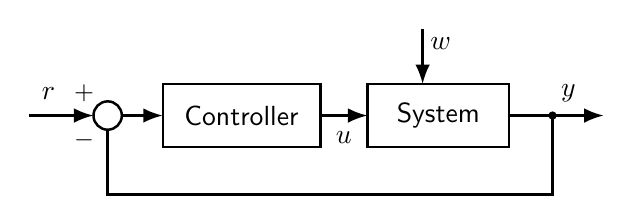
\begin{tikzpicture}[
    >=Latex,
    line width=0.9pt,
    font=\sffamily
]

% Summing junction
\draw (0,0) circle (0.18);

% Plus and minus signs
\node at (-0.3,0.28) {\small $+$};
\node at (-0.3,-0.32) {\small $-$};

% Controller block
\draw (0.7,-0.4) rectangle (2.7,0.4);
\node at (1.7,0) {Controller};

% System block
\draw (3.3,-0.4) rectangle (5.1,0.4);
\node at (4.2,0) {System};

% Input r
\draw[->] (-1.0,0) -- (-0.18,0);
\node at (-0.75,0.28) {$r$};

% From summing junction to controller
\draw[->] (0.18,0) -- (0.7,0);

% Controller to system
\draw[->] (2.7,0) -- (3.3,0);
\node at (3.0,-0.28) {$u$};

% Disturbance w
\draw[->] (4.0,1.1) -- (4.0,0.4);
\node at (4.23,0.92) {$w$};

% Output y
\draw[->] (5.1,0) -- (6.3,0);
\node at (5.85,0.28) {$y$};

% Output node
\fill (5.65,0) circle (1.5pt);

% Feedback path
\draw (5.65,0) -- (5.65,-1.0) -- (0,-1.0) -- (0,-0.18);

\end{tikzpicture}
    \caption{Dual-ascent interpretation of a classical feedback loop. For the linear steady-state relation $y=Hu+w$, primal minimization combined with dual ascent leads to a control law with a proportional term acting on the current tracking error and an integral term represented by the dual variable $\lambda_k$.}
    \label{fig:dual-ascent-pi}
\end{figure}

\subsection{Design insights}
\subsubsection{Design guidelines and tradeoffs}

We can now summarize the main design options discussed so far for online feedback optimization. The three classes of methods considered in this chapter are:
\begin{itemize}
    \item penalty-based gradient methods;
    \item projected-gradient methods;
    \item primal--dual or saddle-flow methods.
\end{itemize}
All three rely on the same basic ingredients:
\begin{itemize}
    \item a fast and stable plant, so that the steady-state map is the relevant object;
    \item some model information in the form of steady-state sensitivities
    \[
    \nabla_u h(u;w);
    \]
    \item output measurements $y$, which provide the feedback signal correcting the optimization step online.
\end{itemize}
What changes is how the constraints are handled, and this leads to different practical tradeoffs.

\paragraph{Penalty methods.}
Penalty methods incorporate the output constraint into the objective. Their main advantage is simplicity: one obtains a smooth unconstrained optimization law, often easy to implement and analyze. Moreover, constraint violation can be made arbitrarily small by choosing a sufficiently strong penalty. However, the violation is not removed exactly, only discouraged. In this sense, the behavior is essentially \emph{proportional}: the correction grows with the violation, but there is no internal memory dedicated to enforcing exact feasibility. A second drawback is that a very steep penalty slows down the optimization dynamics and may lead to poor numerical conditioning or conservative steps.

\paragraph{Projected-gradient methods.}
Projected-gradient methods enforce feasibility more directly. By projecting the update onto an admissible set, they can guarantee \emph{any-time feasibility}, at least with respect to the approximated constraint set used in the projection. This is very attractive when violating constraints is unacceptable. The price to pay is that one must solve a projection problem, which in practice often becomes a quadratic program. So feasibility is improved, but the controller is computationally heavier. In addition, the admissible stepsize is typically limited by the geometry of the projection and by the accuracy of the local approximation.

\paragraph{Saddle-flow or primal--dual methods.}
Primal--dual methods handle the constraints through dual variables. Their main advantage is that feasibility is enforced asymptotically through the multiplier dynamics. The dual variable acts as an integral memory, which is why these methods are often reminiscent of proportional--integral control. This makes them conceptually very appealing and often robust. On the other hand, because of the coupled primal and dual dynamics, oscillations may arise, especially if the gains are not tuned carefully or if the time scales of plant and optimizer are not sufficiently separated.

So the three approaches can be summarized as follows:
\begin{itemize}
    \item \textbf{Penalty:} small violation allowed, simple structure, but steep penalties reduce speed;
    \item \textbf{Projected gradient:} feasibility enforced at every iteration, but requires repeated projection or quadratic programming;
    \item \textbf{Saddle flow / primal--dual:} feasibility obtained asymptotically through an integral-like mechanism, but oscillations may appear.
\end{itemize}

There is therefore no universally best design. The choice depends on the application requirements:
\begin{itemize}
    \item if small temporary violations are acceptable and simplicity is important, penalty methods are attractive;
    \item if feasibility must be guaranteed at all times, projected-gradient methods are preferable;
    \item if one wants a dynamic mechanism that drives the system asymptotically to the constrained optimum, primal--dual methods are natural.
\end{itemize}

This comparison also clarifies the relation with classical control intuition:
\begin{itemize}
    \item penalty methods behave in a mainly proportional way;
    \item primal--dual methods introduce an integral state through the multiplier;
    \item projected-gradient methods correspond instead to explicit feasibility correction through projection.
\end{itemize}

\begin{figure}[!h]
    \centering
    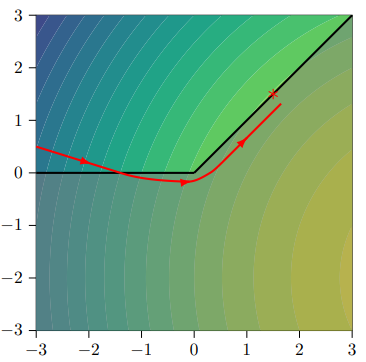
\includegraphics[width=.32\textwidth]{images/feedback_opt_08.png}
    \hfill
    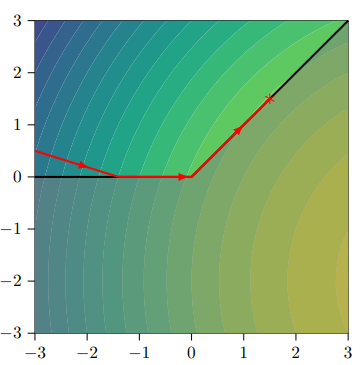
\includegraphics[width=.32\textwidth]{images/feedback_opt_09.png}
    \hfill
    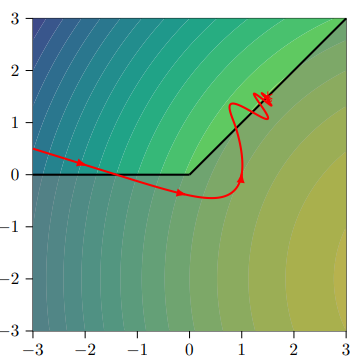
\includegraphics[width=.32\textwidth]{images/feedback_opt_10.png}
    \caption{Qualitative comparison of the trajectories produced by penalty, projected-gradient, and saddle-flow methods. Penalty methods may tolerate small constraint violations, projected-gradient methods maintain feasibility through projection, and saddle-flow methods approach feasibility asymptotically but may exhibit oscillatory behavior.}
    \label{fig:feedback-optimization-tradeoffs}
\end{figure}

In all cases, the same general message remains valid: feedback optimization does not require a full dynamical model of the plant, but it does require the right steady-state information. The central ingredients are the output measurements and the steady-state sensitivity matrix
\[
\nabla_u h(u;w),
\]
which together make it possible to embed optimization algorithms directly into the feedback loop.

\subsection{Extremum seeking}
\subsubsection{Extremum seeking}
So far, all feedback-optimization schemes relied on at least some approximate knowledge of the steady-state sensitivities
\[
\nabla_u h(u;w),
\]
or, equivalently, of the gradient of the performance map with respect to the input. In many applications, however, this information may be unavailable or too unreliable to be useful. This happens, for instance, when the plant is poorly modeled, when the operating conditions vary significantly over time, or when the steady-state map is known only through empirical performance charts.

This raises a natural question: can we optimize a steady-state performance index without any explicit knowledge of the gradient? Extremum-seeking control answers this question positively. It is a class of \emph{zeroth-order} optimization methods, meaning that it seeks the optimizer by using only measurements of the cost or performance, without requiring an analytical model of its gradient.

The general setting is the following. We consider again a fast stable plant, and we associate to each constant input $u$ a scalar performance metric
\[
J(u),
\]
which we want to minimize or maximize. The key difficulty is that the gradient
\[
\nabla_u J(u)
\]
is unknown. Extremum seeking overcomes this difficulty by injecting a small oscillatory perturbation into the input, observing the corresponding oscillatory component in the measured performance, and extracting from it an estimate of the local gradient.

This is why extremum seeking is often regarded as a learning-based feedback optimizer: it does not need a model of the steady-state sensitivities, because it estimates the necessary descent information online from measured data. In this sense, it complements the methods studied earlier in the chapter. When sensitivities are available, gradient, projected-gradient, or primal--dual methods are natural. When sensitivities are unknown, one may either estimate them or switch to a purely zeroth-order approach such as extremum seeking.

It is worth stressing one important robustness point. Even when the available sensitivity model is very inaccurate, the feedback-optimization schemes discussed previously may still work reasonably well. However, if one wants to avoid relying on such information altogether, extremum seeking is a natural alternative. This is one of the main motivations for introducing it at the end of the chapter.

\paragraph{Exercise.}
A useful fact to check is the following: both projected gradient descent and saddle-flow methods cannot have an equilibrium corresponding to an infeasible steady state
\[
y\notin\mathcal Y.
\]
This reinforces the idea that feedback optimization is structurally tied to feasibility. Extremum seeking, on the other hand, addresses a different issue: not the lack of feasibility mechanisms, but the lack of gradient information.

\subsubsection{Extremum-seeking architecture}

The simplest extremum-seeking idea can be explained for a scalar input. Suppose that the plant is fast and stable, and that the measured steady-state performance is $J(u)$. We want to optimize $J(u)$ without knowing its gradient.

The controller is built around four basic ingredients:
\begin{itemize}
    \item an \emph{exploration signal}, which perturbs the input with a small sinusoid;
    \item a \emph{high-pass filter}, which removes the slowly varying offset in the measured performance;
    \item a \emph{demodulation step}, which multiplies the filtered performance by a sinusoidal signal at the same frequency;
    \item a \emph{low-pass filter} followed by an integrator, which extracts an average descent direction and updates the nominal input.
\end{itemize}

Denoting by $\hat u_k$ the slowly varying nominal input and by $\rho \sin(\omega k)$ the injected perturbation, the actual plant input is
\[
u_k=\hat u_k+\rho \sin(\omega k).
\]
So the plant is continuously excited around the nominal operating point. The purpose of this small oscillation is to probe the local slope of the performance function.

The measured performance $J(u_k)$ is then passed through a high-pass filter, which removes the average component and keeps the oscillatory part induced by the perturbation. This signal is subsequently multiplied by a sinusoid of the same frequency. This multiplication step is often called \emph{demodulation}, because it extracts the component of the output that is correlated with the injected exploration signal. Finally, a low-pass filter removes the high-frequency terms, leaving only a slowly varying approximation of the gradient. The resulting signal is then integrated to update the nominal input $\hat u_k$ in the direction of improvement.

\begin{figure}[!h]
    \centering
    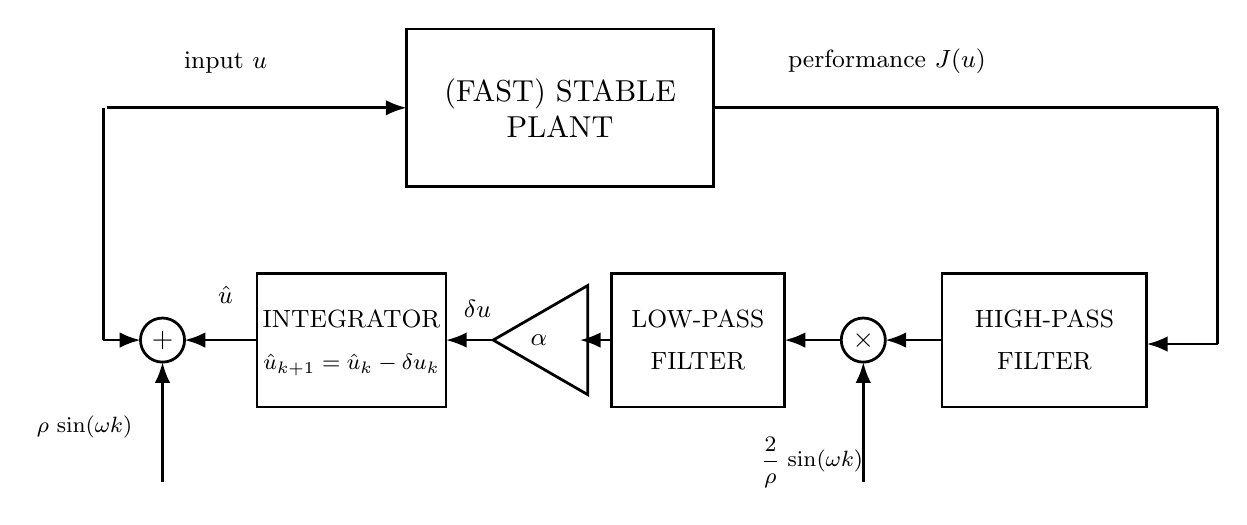
\begin{tikzpicture}[
    >=Latex,
    line width=1pt,
    font=\sffamily
]

%======================
% Top plant block
%======================
\draw (4.3,3.0) rectangle (8.2,5.0);
\node[align=center, font=\fontsize{11}{13}\selectfont] at (6.25,4.0) {(FAST) STABLE\\PLANT};

% Input to plant
\draw[->] (0.5,4.0) -- (4.3,4.0);
\node[above, font=\fontsize{9}{11}\selectfont] at (2.0,4.3) {input $u$};

% Output from plant
\draw[-] (8.2,4.0) -- (14.6,4.0);
\node[above, font=\fontsize{9}{11}\selectfont] at (10.4,4.3) {performance $J(u)$};

% Right vertical return
\draw[-] (14.6,4.0) -- (14.6,1.0);

%======================
% Bottom row blocks
%======================

% Summing node
\draw (1.2,1.05) circle (0.28);
\node at (1.2,1.05) {$+$};

% Integrator
\draw (2.4,0.2) rectangle (4.8,1.9);
\node[align=center, font=\fontsize{9}{11}\selectfont] at (3.6,1.32) {INTEGRATOR};
\node[align=center, font=\fontsize{8}{10}\selectfont] at (3.6,0.73)
{$\hat{u}_{k+1}=\hat{u}_{k}-\delta u_k$};

% Gain triangle (left-pointing)
\node[
    draw,
    isosceles triangle,
    isosceles triangle apex angle=60,
    shape border rotate=180,
    minimum height=1.2cm,
    minimum width=1.0cm,
    inner sep=0pt
] (gain) at (6.2,1.05) {};
\node[font=\fontsize{9}{11}\selectfont] at (5.98,1.05) {$\alpha$};

% Low-pass filter
\draw (6.9,0.2) rectangle (9.1,1.9);
\node[align=center, font=\fontsize{9}{11}\selectfont] at (8.0,1.32) {LOW-PASS};
\node[align=center, font=\fontsize{9}{11}\selectfont] at (8.0,0.78) {FILTER};

% Multiplier
\draw (10.1,1.05) circle (0.28);
\node at (10.1,1.05) {$\times$};

% High-pass filter
\draw (11.1,0.2) rectangle (13.7,1.9);
\node[align=center, font=\fontsize{9}{11}\selectfont] at (12.4,1.32) {HIGH-PASS};
\node[align=center, font=\fontsize{9}{11}\selectfont] at (12.4,0.78) {FILTER};

%======================
% Connections
%======================

% Right return into high-pass
\draw[->] (14.6,1.0) -- (13.7,1.0);

% High-pass to multiplier
\draw[->] (11.1,1.05) -- (10.38,1.05);

% Sine input to multiplier
\draw[->] (10.1,-0.75) -- (10.1,0.77);
\node[below, align=center, font=\fontsize{8}{10}\selectfont] at (9.45,-0.05)
{$\dfrac{2}{\rho}\,\sin(\omega k)$};

% Multiplier to low-pass
\draw[->] (9.82,1.05) -- (9.1,1.05);

% Low-pass to gain
\draw[->] (6.9,1.05) -- (6.5,1.05);
\node[above, font=\fontsize{9}{11}\selectfont] at (5.2,1.2) {$\delta u$};

% Gain to integrator
\draw[->] (5.38,1.05) -- (4.8,1.05);

% Integrator to summing node
\draw[->] (2.4,1.05) -- (1.48,1.05);
\node[above, font=\fontsize{9}{11}\selectfont] at (2.0,1.38) {$\hat{u}$};

% Sine input to summing node
\draw[->] (1.2,-0.75) -- (1.2,0.77);
\node[left, font=\fontsize{8}{10}\selectfont] at (0.95,-0.05) {$\rho\,\sin(\omega k)$};

% Summing node to plant input path
\draw[-] (0.45,1.05) -- (0.45,4.0);
\draw[->] (0.45,1.05) -- (0.92,1.05);

\end{tikzpicture}
    \caption{Basic extremum-seeking architecture. A small sinusoidal perturbation is added to the nominal input $\hat u_k$ in order to explore the local slope of the steady-state performance $J(u)$. The measured performance is high-pass filtered, demodulated, low-pass filtered, and finally integrated so as to generate an update of the nominal input.}
    \label{fig:extremum-seeking-architecture}
\end{figure}

The exploration signal
\[
\rho \sin(\omega k)
\]
should be thought of as a deliberate excitation used to reveal local gradient information. The demodulation signal, typically proportional to
\[
\frac{2}{\rho}\sin(\omega k),
\]
is chosen so that, after averaging, the product isolates the first-order term of the Taylor expansion of the performance function.

So the overall architecture can be interpreted as a feedback mechanism that reconstructs a gradient estimate from input--output oscillations, without ever requiring an explicit model of the plant or of the performance map.

\subsubsection{Why extremum seeking behaves like gradient descent}

The basic mechanism can be understood with a first-order Taylor expansion. Starting from
\[
u_k=\hat u_k+\rho \sin(\omega k),
\]
assume that $\rho$ is small, so that the performance function can be expanded around the nominal input:
\[
J(u_k)\approx J(\hat u_k)+\nabla_u J(\hat u_k)\,\rho \sin(\omega k).
\]
The first term is a slowly varying offset, while the second is an oscillatory term whose amplitude is proportional to the unknown gradient.

After the high-pass filter, the offset is removed, and we are left approximately with
\[
\nabla_u J(\hat u_k)\,\rho \sin(\omega k).
\]
The next step is demodulation. Multiplying by
\[
\frac{2}{\rho}\sin(\omega k)
\]
gives
\[
\nabla_u J(\hat u_k)\, 2\sin^2(\omega k).
\]
Using the identity
\[
2\sin^2(\omega k)=1-\cos(2\omega k),
\]
we see that this signal consists of a constant part,
\[
\nabla_u J(\hat u_k),
\]
plus a fast oscillation at frequency $2\omega$. The low-pass filter removes the oscillatory component and keeps only the average value. Therefore, after the low-pass filter, the signal is approximately
\[
\nabla_u J(\hat u_k).
\]

If this signal is then multiplied by a gain $\alpha$, we obtain the update direction
\[
\delta u_k=\alpha \nabla_u J(\hat u_k).
\]
Finally, the integrator implements
\[
\hat u_{k+1}=\hat u_k-\delta u_k,
\]
hence
\[
\hat u_{k+1}=\hat u_k-\alpha \nabla_u J(\hat u_k).
\]
But this is exactly the gradient-descent iteration.

So, at an intuitive level, extremum seeking is nothing but gradient descent in disguise:
\begin{itemize}
    \item the exploration signal reveals the local slope of the performance map;
    \item the filtering and demodulation reconstruct the gradient;
    \item the integrator performs the actual descent step.
\end{itemize}

Of course, this derivation is only a sketch. A rigorous analysis requires averaging arguments, time-scale separation, and assumptions on the filters and on the plant dynamics. But the basic idea is exactly the one above: extremum seeking creates its own gradient information through oscillatory probing.

\subsubsection{Applications of extremum seeking}

Extremum seeking is especially attractive in applications with the following features:
\begin{itemize}
    \item the plant is fast and stable at the time scale of the optimizer;
    \item the steady-state performance map is poorly known or strongly parameter dependent;
    \item the optimization problem is low dimensional;
    \item small oscillatory perturbations of the input are acceptable.
\end{itemize}

A classical example is photovoltaic maximum-power-point tracking. In a photovoltaic system, the active power generated by the panel depends on the operating voltage, and the power--voltage curve changes significantly with solar irradiance and temperature. Therefore, the location of the optimal voltage is not fixed and may vary continuously during operation. Moreover, an accurate model of the full dependence on the environmental variables may be difficult to maintain online.

In this situation, extremum seeking is very natural. By slightly perturbing the voltage and measuring the resulting power, the controller can estimate whether the current operating point is to the left or to the right of the maximum, and then move the nominal voltage in the correct direction. In this way, the controller tracks the operating voltage that maximizes active power generation without requiring an explicit gradient model.

This is a particularly good use case because:
\begin{itemize}
    \item the optimum varies with exogenous conditions;
    \item the model is poor or uncertain;
    \item the control input is low dimensional;
    \item the actuator cost of a small oscillatory probing signal is acceptable.
\end{itemize}

Other relevant applications include internal combustion engines, chemical processes, compressor systems, and meta-optimization problems such as tuning controller parameters. In all these cases, extremum seeking is valuable when the optimizer can rely on measured performance only, while the gradient or the steady-state sensitivity is unavailable.

\paragraph{Final perspective.}
This closes the chapter with an important conceptual message. Feedback optimization can be organized along a spectrum:
\begin{itemize}
    \item if reliable steady-state sensitivities are available, one can use gradient, projected-gradient, or primal--dual schemes;
    \item if sensitivities are inaccurate, one may still rely on robust feedback optimization based on approximate models;
    \item if sensitivities are completely unknown, one can move to learning or zeroth-order methods such as extremum seeking.
\end{itemize}

So extremum seeking is not a separate topic disconnected from the rest. It is the natural endpoint of the feedback-optimization viewpoint: when model-based gradient information disappears, the controller can still recover optimization directions directly from feedback measurements.
\newpage

\section{System Identification}
So far, the control methods that we have studied, in particular LQR and Model Predictive Control, have relied on the availability of a state-space model of the plant. In discrete time, this is typically written as
\[
x_{t+1} = A x_t + B u_t, 
\qquad
y_t = C x_t,
\]
or, more generally, with a nonlinear update map. This representation is extremely convenient for control design, because it provides a Markovian description of the system: once the current state is known, the future evolution depends only on the present state and on the input that will be applied. In this sense, the state is the variable that summarizes all the information from the past that is relevant for predicting the future.

Having such a model, however, means having a very detailed description of the plant. One must know the parameters that govern the state update, the way in which the input affects the state evolution, and the way in which the internal state is mapped into the measured outputs. Even more fundamentally, one must decide what the state actually is, that is, which variables are sufficient to obtain a Markovian model. This is already a nontrivial modeling choice, especially when the internal physical variables are not directly measurable.

A first important observation is that a state-space representation is not unique. Different internal coordinates may describe exactly the same external input-output behavior. Indeed, if we introduce a new state variable \(w_t\) through an invertible linear change of coordinates
\[
x_t = T w_t,
\]
with \(T\) nonsingular, then the system can be equivalently written as
\[
w_{t+1} = T^{-1} A T w_t + T^{-1} B u_t,
\qquad
y_t = C T w_t.
\]
Although the matrices appearing in the model have changed, the input-output trajectories remain exactly the same. Therefore, the state should not be interpreted as a uniquely defined physical object, but rather as an internal variable that makes prediction and control possible. What really matters from the external viewpoint is the input-output behavior of the system.

This point is one of the main motivations for system identification. If different state-space models can generate the same measured behavior, then reconstructing a model from data cannot be understood as recovering the ``true'' internal realization in an absolute sense. Instead, the goal is to build a model that reproduces the observed dynamics well enough for the intended task. In our context, this task is control. Therefore, the identified model should be sufficiently accurate to predict the future effect of the control inputs and to support the synthesis of model-based controllers.

System identification addresses exactly this problem. Rather than deriving the model entirely from first principles, we use measured input-output data to infer a dynamical description of the plant. This is especially useful when a first-principles model is unavailable, too expensive to derive, or too inaccurate for control purposes. The identified model may be a state-space realization, an input-output model, or another predictive representation, depending on the assumptions and on the control architecture of interest.

From this viewpoint, identification can be seen as the bridge between data and model-based control. On the one hand, advanced controllers such as LQR and MPC require a predictive model. On the other hand, the model need not be known a priori: it can be estimated from experiments. The central question of this chapter is therefore how to extract, from measured data, a model that captures the relevant dynamical behavior of the plant and can be reliably used for prediction and control.

A natural way to move from an internal state-space description to an external input-output description is to write the output as a function of the initial condition and of the past inputs. For the discrete-time linear system
\[
x_{t+1}=Ax_t+Bu_t,\qquad y_t=Cx_t,
\]
repeated substitution gives
\[
y_t = CA^t x_0 + \sum_{j=0}^{t-1} CA^{\,t-1-j} B\,u_j.
\]
This expression clearly separates two contributions. The term \(CA^t x_0\) is the response generated by the initial state, while the summation describes how past inputs are propagated to the output through the dynamics. The latter has the form of a discrete-time convolution and shows that, for linear time-invariant systems, the full input-output behavior is encoded in the sequence of matrices
\[
CA^{t-1}B,\qquad t>0.
\]

In the SISO case, where both \(u_t\in\mathbb{R}\) and \(y_t\in\mathbb{R}\), this sequence reduces to a scalar sequence
\[
h_t = CA^{t-1}B,\qquad t>0,
\]
which is the impulse response of the system. If the initial condition is zero, then the output produced by an arbitrary input sequence is completely determined by the convolution of the input with \(\{h_t\}_{t\geq 1}\). In this sense, the impulse response is a complete representation of the zero-state input-output map of the plant. It contains exactly the information needed to predict future outputs from past inputs, without explicitly referring to the internal state coordinates. This is especially important in identification, because the state itself is not directly unique, whereas the input-output behavior is the physically observable object.

The same idea extends immediately to MIMO systems. If the plant has \(m\) inputs and \(p\) outputs, then each coefficient
\[
H_t = CA^{t-1}B \in \mathbb{R}^{p\times m},\qquad t>0,
\]
is a matrix. Its entry in position \((i,j)\) represents the response of output \(i\) to a unit impulse applied on input \(j\). The sequence \(\{H_t\}_{t\geq 1}\) is called the sequence of Markov parameters of the system. These parameters generalize the impulse response and provide a compact description of the input-output behavior of the linear system. Once they are known, the output can be reconstructed from the past inputs through matrix convolution.

This viewpoint is also attractive from an experimental perspective. On a real plant, the Markov parameters can be estimated directly from data by exciting the system and measuring the corresponding outputs. In the ideal noise-free case, one can initialize the plant at zero and apply a unit impulse to one input channel at a time, while keeping the others equal to zero. For a MIMO system, this means that \(m\) experiments are sufficient in principle: each experiment isolates one column of the matrices \(H_t\), and by repeating the procedure for all inputs one reconstructs the full sequence of Markov parameters. In practice, however, perfect impulses cannot be generated and measurements are affected by noise, disturbances, and possible offsets in the initial condition. For this reason, identification methods usually rely on richer input signals and estimate the Markov parameters from batches of input-output data, rather than from a single idealized impulse experiment.

The key message is that, before identifying a state-space realization, one may already identify the external behavior of the plant through its impulse response, or equivalently through its Markov parameters. This provides the first bridge between measured data and predictive models, and it motivates the identification techniques developed in the rest of this chapter.

\subsection{Controllability, observability, and minimal realizations}

When the goal is to identify a state-space model from input-output data, not every realization is equally meaningful. Since the state is not unique, one can always introduce additional coordinates that do not change the external behavior of the system. For identification and control, however, we are interested in realizations in which the state has an actual dynamical role. This naturally leads to the notions of controllability and observability, which characterize whether the state can be influenced by the input and reconstructed from the output.

For the discrete-time linear system
\[
x_{t+1}=Ax_t+Bu_t,\qquad y_t=Cx_t,
\]
controllability concerns the possibility of steering the system from a given initial condition to a desired target state. To fix ideas, let us start from \(x_0=0\). After one step, the state is
\[
x_1 = Bu_0,
\]
so the set of states reachable in one step is exactly the image of \(B\). After two steps,
\[
x_2 = ABu_0 + Bu_1,
\]
hence the reachable set is the image of the matrix \([\,B\;\;AB\,]\). Continuing in the same way, after \(n\) steps the state belongs to the image of
\[
\mathcal{C} = \begin{bmatrix} B & AB & A^2B & \cdots & A^{n-1}B \end{bmatrix},
\]
which is called the controllability matrix. Therefore, the system is controllable precisely when every state in \(\mathbb{R}^n\) can be reached, that is, when
\[
\operatorname{rank}(\mathcal{C}) = n.
\]
This condition means that the columns generated by repeatedly propagating the input directions through the dynamics span the whole state space. It is worth stressing that \(n\) steps are enough to decide controllability: if the full state space has not been reached by then, taking more steps cannot generate new independent directions.

The controllability matrix also provides a constructive way to compute a control sequence that reaches a desired state. Indeed, for a target \(\bar x\) reached in \(n\) steps, one can write
\[
x_n = \mathcal{C}
\begin{bmatrix}
u_{n-1}\\
\vdots\\
u_0
\end{bmatrix}.
\]
If \(\mathcal{C}\) is square and invertible, which is possible in particular in the scalar-input case, the input sequence is obtained directly by inversion. In the more general case, \(\mathcal{C}\) is not square, and the problem may admit multiple solutions. A standard choice is then the minimum-norm solution, which can be computed through the pseudoinverse.

Dual to controllability is observability. While controllability asks whether the input can excite all internal directions, observability asks whether the effect of the initial state can be detected from the output. Starting again from the linear model, at time \(t=0\) one has
\[
y_0 = Cx_0,
\]
so any initial state in the kernel of \(C\) is invisible at the output at that instant. After one step,
\[
y_1 = CAx_0,
\]
hence a state that belongs simultaneously to the kernels of \(C\) and \(CA\) remains indistinguishable over the first two output samples. Proceeding recursively, after \(n\) steps the invisible states are those in the kernel of
\[
\mathcal{O}=
\begin{bmatrix}
C\\
CA\\
CA^2\\
\vdots\\
CA^{n-1}
\end{bmatrix},
\]
which is called the observability matrix. The system is observable if and only if
\[
\operatorname{rank}(\mathcal{O})=n.
\]
Equivalently, distinct initial states always generate distinct output trajectories over a finite observation window. Also here, \(n\) steps are sufficient: if a state cannot be distinguished from the output sequence of length \(n\), it will remain unobservable even if more measurements are collected.

As in the controllability case, observability has a constructive interpretation. Given an output sequence \(y_0,\dots,y_{n-1}\), one can write
\[
\begin{bmatrix}
y_0\\
y_1\\
\vdots\\
y_{n-1}
\end{bmatrix}
=
\mathcal{O}x_0.
\]
If \(\mathcal{O}\) is invertible, the initial state is uniquely determined. More generally, when \(\mathcal{O}\) has full column rank, the state can still be reconstructed uniquely, for instance through a least-squares inversion based on the pseudoinverse.

These two notions are central in system identification because they single out the realizations that are meaningful from input-output data. If a realization contains uncontrollable states, part of the state cannot be influenced by the input and is therefore irrelevant for prediction and control. If it contains unobservable states, part of the state has no effect on the measured output and therefore cannot be inferred from data. In both cases, the realization contains redundant internal coordinates. For this reason, in identification we focus on realizations that are both controllable and observable. Such realizations are called minimal, because they do not contain superfluous states and represent the input-output behavior with the smallest possible state dimension.

A simple example illustrates the point. Consider a plant whose output is a moving average of the past three inputs,
\[
y_t = a_1u_{t-1}+a_2u_{t-2}+a_3u_{t-3}.
\]
A natural state is obtained by storing delayed copies of the input:
\[
x_t=
\begin{bmatrix}
u_{t-1}\\
u_{t-2}\\
u_{t-3}
\end{bmatrix}.
\]
With this choice, the dynamics become
\[
x_{t+1}
=
\begin{bmatrix}
0&0&0\\
1&0&0\\
0&1&0
\end{bmatrix}x_t
+
\begin{bmatrix}
1\\
0\\
0
\end{bmatrix}u_t,
\qquad
y_t=
\begin{bmatrix}
a_1 & a_2 & a_3
\end{bmatrix}x_t.
\]
This realization has an immediate interpretation: the state is simply a memory of the past input values needed to compute the current output.

The controllability matrix of this realization is
\[
\mathcal{C}=
\begin{bmatrix}
B & AB & A^2B
\end{bmatrix}=I,
\]
so the system is controllable. This is consistent with the physical meaning of the state, since the input directly writes the first memory cell and, through the shift dynamics, can generate any delayed input profile. The observability matrix is
\[
\mathcal{O}=
\begin{bmatrix}
a_1 & a_2 & a_3\\
a_2 & a_3 & 0\\
a_3 & 0 & 0
\end{bmatrix}.
\]
Hence observability depends on the coefficients \(a_1,a_2,a_3\). When this matrix has full rank, the three stored delays all leave a visible signature in the output and the realization is minimal. If instead the rank is smaller, then some component of the chosen state does not affect the output independently, which means that a lower-order realization exists.

This example clarifies why controllability and observability are so important in identification. Starting from input-output data, one does not want to recover an arbitrary realization, but rather a realization whose state is both reachable from the input and visible from the output. Only in this case does the state provide a well-posed internal representation of the external behavior of the plant, and only in this case can we hope to obtain a compact and useful model for control design.

\subsection{Realization from data and the Ho--Kalman construction}

The discussion so far has shown that the input-output behavior of a linear time-invariant system is completely described by its Markov parameters
\[
\{CB,\;CAB,\;CA^2B,\;\dots\}.
\]
This naturally leads to the realization problem: if these parameters are known from experiments, how can one reconstruct a state-space model
\[
x_{t+1}=Ax_t+Bu_t,\qquad y_t=Cx_t
\]
that generates them? More generally, given generic input-output data, how can one construct a realization \(A,B,C\) consistent with the observed dynamics? The goal is not to recover a unique internal state, since different state-space models may have the same external behavior, but rather to compute a minimal realization, that is, one that is both controllable and observable.

The key object in this construction is the Hankel matrix built from the Markov parameters. If we define the observability and controllability matrices of a minimal realization as
\[
\mathcal{O}=
\begin{bmatrix}
C\\
CA\\
CA^2\\
\vdots\\
CA^{n-1}
\end{bmatrix},
\qquad
\mathcal{C}=
\begin{bmatrix}
B & AB & A^2B & \cdots & A^{n-1}B
\end{bmatrix},
\]
then their product is
\[
\mathcal{H}=\mathcal{O}\mathcal{C}.
\]
Expanding this product shows that every block of \(\mathcal{H}\) is one of the Markov parameters:
\[
\mathcal{H}=
\begin{bmatrix}
CB & CAB & CA^2B & \cdots & CA^{n-1}B\\
CAB & CA^2B & CA^3B & \cdots & CA^nB\\
CA^2B & CA^3B & CA^4B & \cdots & CA^{n+1}B\\
\vdots & \vdots & \vdots & \ddots & \vdots\\
CA^{n-1}B & CA^nB & CA^{n+1}B & \cdots & CA^{2n-2}B
\end{bmatrix}.
\]
Thus the Hankel matrix can be assembled directly from experimental data as soon as enough Markov parameters are available. This is the crucial bridge between input-output measurements and state-space realizations.

To make the structure visually apparent, it is often helpful to highlight repeated Markov parameters along the anti-diagonals. For example, one may write
\[
\mathcal{H}=
\left[
\begin{array}{ccccc}
\colorbox{red!20}{$CB$} &
\colorbox{blue!20}{$CAB$} &
\colorbox{green!20}{$CA^2B$} &
\cdots &
CA^{n-1}B\\[0.3em]
\colorbox{blue!20}{$CAB$} &
\colorbox{green!20}{$CA^2B$} &
CA^3B &
\cdots &
CA^nB\\[0.3em]
\colorbox{green!20}{$CA^2B$} &
CA^3B &
CA^4B &
\cdots &
CA^{n+1}B\\
\vdots & \vdots & \vdots & \ddots & \vdots\\
CA^{n-1}B & CA^nB & CA^{n+1}B & \cdots & CA^{2n-2}B
\end{array}
\right].
\]
The repeated colors emphasize that each anti-diagonal contains the same Markov parameter. This is exactly the signature of a Hankel structure: the matrix is constant along anti-diagonals, and those constants are the impulse-response coefficients of the system.

The Ho--Kalman algorithm uses this structure in three conceptual steps. First, one constructs the Hankel matrix from the measured Markov parameters. Second, one factorizes the Hankel matrix as
\[
\mathcal{H}=\mathcal{O}\mathcal{C}.
\]
Third, one extracts a realization \(A,B,C\) from the factors \(\mathcal{O}\) and \(\mathcal{C}\).

At first sight, the first step raises a basic difficulty: how many Markov parameters are needed? The answer depends on the order \(n\) of the minimal realization, which is unknown a priori. However, if the realization is minimal, then both \(\mathcal{O}\) and \(\mathcal{C}\) have rank \(n\), and therefore the Hankel matrix also has rank \(n\). This means that, in principle, one can enlarge the Hankel matrix progressively until its rank stops increasing. That plateau reveals the order of the system. In noise-free settings this idea works exactly; in practice, with noisy data, the same principle survives in approximate form and the effective rank is inferred numerically.

This rank-based interpretation is easy to understand on simple examples. A first-order low-pass filter has state-space model
\[
x_{t+1}=ax_t+u_t,\qquad y_t=x_t,
\]
so its Markov parameters are \(1,a,a^2,\dots\), and the corresponding Hankel matrix has rank one. By contrast, a frictionless cart model written as
\[
v_{t+1}=v_t+u_t,\qquad z_{t+1}=z_t+v_t,\qquad y_t=z_t
\]
has a two-dimensional state, and the Hankel matrix reflects this higher order through rank two. In this way, the rank of the Hankel matrix captures the intrinsic dimension of the minimal realization.

The second step of the Ho--Kalman method is the factorization
\[
\mathcal{H}=\mathcal{O}\mathcal{C}.
\]
An important conceptual point is that this factorization is not unique, but this is not a problem. Indeed, nonuniqueness of the factorization simply reflects nonuniqueness of the state coordinates. If we apply a change of basis
\[
\tilde A = T^{-1}AT,\qquad \tilde B = T^{-1}B,\qquad \tilde C = CT,
\]
with \(T\) invertible, then the corresponding observability and controllability matrices become
\[
\tilde{\mathcal{O}}=
\begin{bmatrix}
\tilde C\\
\tilde C\tilde A\\
\tilde C\tilde A^2\\
\vdots
\end{bmatrix}
=
\begin{bmatrix}
CT\\
CTA T^{-1}T\\
CTA^2T^{-1}T\\
\vdots
\end{bmatrix}
=
\mathcal{O}T,
\]
and similarly
\[
\tilde{\mathcal{C}}=T^{-1}\mathcal{C}.
\]
Therefore,
\[
\tilde{\mathcal{O}}\tilde{\mathcal{C}}
=
\mathcal{O}TT^{-1}\mathcal{C}
=
\mathcal{O}\mathcal{C}
=
\mathcal{H}.
\]
So different factorizations of \(\mathcal{H}\) correspond exactly to different coordinate representations of the same input-output system. The factorization does not identify a unique realization, but it identifies the system up to similarity transformation, which is the correct notion of uniqueness for state-space models.

Because of this, the factorization step leaves some freedom. In principle, one could take trivial choices such as \(\mathcal{O}=I\) and \(\mathcal{C}=\mathcal{H}\), or \(\mathcal{O}=\mathcal{H}\) and \(\mathcal{C}=I\), but these choices are not useful numerically and do not directly reveal a well-scaled state representation. In practice, one prefers factorizations based on the singular value decomposition, because they expose the rank of the Hankel matrix and provide numerically robust coordinates for the state.

Once a factorization \(\mathcal{H}=\mathcal{O}\mathcal{C}\) has been obtained, the realization matrices are recovered from the shift structure of \(\mathcal{O}\) and \(\mathcal{C}\). The matrix \(C\) is simply the first block row of \(\mathcal{O}\), while \(B\) is the first block column of \(\mathcal{C}\). The state transition matrix \(A\) is then determined by exploiting the fact that consecutive block rows of \(\mathcal{O}\) differ by multiplication by \(A\), or equivalently that consecutive block columns of \(\mathcal{C}\) differ by the same shift. In this way, the whole state-space realization is reconstructed from the Hankel matrix, and therefore from measured input-output behavior alone.

The significance of the Ho--Kalman construction is that it turns impulse-response data into a minimal state-space model through linear-algebraic operations. It provides one of the cleanest answers to the realization problem: first identify the Markov parameters, then organize them into a Hankel matrix, then factorize this matrix to uncover the underlying controllable and observable state structure.

\subsection{SVD-based Ho--Kalman realization}

The key missing ingredient in the Ho--Kalman construction is a numerically reliable way to factorize the Hankel matrix. This is provided by the singular value decomposition. If \(H\in\mathbb{R}^{m\times n}\) has rank \(r\), then it can be written as
\[
H = U\Sigma V^\top,
\]
where \(U\in\mathbb{R}^{m\times m}\) and \(V\in\mathbb{R}^{n\times n}\) are orthogonal matrices, while \(\Sigma\in\mathbb{R}^{m\times n}\) is diagonal in the rectangular sense, with nonnegative singular values on the diagonal. If the rank of \(H\) is \(r\), then only the first \(r\) singular values are nonzero, and the decomposition can be partitioned as
\[
H=
\begin{bmatrix}
U_1 & U_2
\end{bmatrix}
\begin{bmatrix}
\Sigma_1 & 0\\
0 & 0
\end{bmatrix}
\begin{bmatrix}
V_1 & V_2
\end{bmatrix}^{\!\top}
=
U_1\Sigma_1V_1^\top,
\]
where \(\Sigma_1\in\mathbb{R}^{r\times r}\) contains the nonzero singular values. This decomposition is one of the most useful tools in numerical linear algebra: it is computationally efficient, numerically robust, and it reveals directly the rank and the dominant subspaces of the matrix. In particular, the columns of \(U_1\) span the image of \(H\), while the dimension of \(\Sigma_1\) identifies the rank.

This is exactly the type of factorization we need for the Hankel matrix. Instead of building a square Hankel matrix of unknown dimension, it is convenient to introduce an extended Hankel matrix
\[
\mathcal{H}_{k,\ell}=
\begin{bmatrix}
G_1 & G_2 & \cdots & G_\ell\\
G_2 & G_3 & \cdots & G_{\ell+1}\\
G_3 & G_4 & \cdots & G_{\ell+2}\\
\vdots & \vdots & \ddots & \vdots\\
G_k & G_{k+1} & \cdots & G_{k+\ell-1}
\end{bmatrix},
\]
where \(G_t = CA^{t-1}B\) denotes the \(t\)-th Markov parameter. Here \(k\) and \(\ell\) are chosen larger than the unknown system order \(n\). If the data are generated by an \(n\)-dimensional minimal realization, then this extended Hankel matrix factors as
\[
\mathcal{H}_{k,\ell}=\mathcal{O}_k\mathcal{C}_\ell,
\]
with
\[
\mathcal{O}_k=
\begin{bmatrix}
C\\
CA\\
CA^2\\
\vdots\\
CA^{k-1}
\end{bmatrix},
\qquad
\mathcal{C}_\ell=
\begin{bmatrix}
B & AB & A^2B & \cdots & A^{\ell-1}B
\end{bmatrix}.
\]
These are the extended observability and controllability matrices. As soon as \(k\ge n\) and \(\ell\ge n\), both matrices have rank \(n\), and therefore \(\mathcal{H}_{k,\ell}\) also has rank \(n\). This is the fundamental reason why one chooses \(k\) and \(\ell\) larger than the system order: once the horizon is long enough, the rank of the Hankel matrix reveals the true dimension of the minimal realization.

At this point, the SVD gives a natural and balanced factorization of \(\mathcal{H}_{k,\ell}\). If
\[
\mathcal{H}_{k,\ell}=U_1\Sigma_1V_1^\top,
\]
where \(\Sigma_1\) contains the nonzero singular values, then the order of the system is simply
\[
n=\operatorname{rank}(\mathcal{H}_{k,\ell})=\dim(\Sigma_1).
\]
Moreover, we may decompose the Hankel matrix as
\[
\mathcal{H}_{k,\ell}
=
\underbrace{U_1\Sigma_1^{1/2}}_{\mathcal{O}_k}
\underbrace{\Sigma_1^{1/2}V_1^\top}_{\mathcal{C}_\ell}.
\]
This choice is especially convenient because it distributes the scaling symmetrically between the observability and controllability factors. In this way we obtain numerical representatives of the extended observability and controllability matrices:
\[
\mathcal{O}_k = U_1\Sigma_1^{1/2},
\qquad
\mathcal{C}_\ell = \Sigma_1^{1/2}V_1^\top.
\]

From these matrices, \(C\) and \(B\) are obtained immediately. Indeed, \(C\) is the first block row of \(\mathcal{O}_k\), while \(B\) is the first block column of \(\mathcal{C}_\ell\). Visually, one can emphasize this as
\[
\mathcal{O}_k=
\begin{bmatrix}
\colorbox{green!20}{$C$}\\
CA\\
CA^2\\
\vdots\\
CA^{k-1}
\end{bmatrix},
\qquad
\mathcal{C}_\ell=
\begin{bmatrix}
\colorbox{green!20}{$B$} & AB & A^2B & \cdots & A^{\ell-1}B
\end{bmatrix}.
\]
Thus the first visible block of the observability factor gives the output matrix, and the first visible block of the controllability factor gives the input matrix.

To recover the state transition matrix \(A\), one introduces the shifted Hankel matrix
\[
\mathcal{H}^{\uparrow}_{k,\ell}=
\begin{bmatrix}
G_2 & G_3 & \cdots & G_{\ell+1}\\
G_3 & G_4 & \cdots & G_{\ell+2}\\
G_4 & G_5 & \cdots & G_{\ell+3}\\
\vdots & \vdots & \ddots & \vdots\\
G_{k+1} & G_{k+2} & \cdots & G_{k+\ell}
\end{bmatrix}.
\]
By construction, this matrix satisfies
\[
\mathcal{H}^{\uparrow}_{k,\ell}=
\begin{bmatrix}
CAB & CA^2B & CA^3B & \cdots\\
CA^2B & CA^3B & CA^4B & \cdots\\
CA^3B & CA^4B & CA^5B & \cdots\\
\vdots & \vdots & \vdots & \ddots
\end{bmatrix}
=
\mathcal{O}_k A \mathcal{C}_\ell.
\]
Once \(\mathcal{O}_k\) and \(\mathcal{C}_\ell\) are known, this relation can be inverted in the least-squares sense, yielding
\[
A = \mathcal{O}_k^\dagger \mathcal{H}^{\uparrow}_{k,\ell}\mathcal{C}_\ell^\dagger,
\]
where \({}^\dagger\) denotes the pseudoinverse. Therefore the full realization \((A,B,C)\) is reconstructed directly from the measured Markov parameters.

Putting everything together, the Ho--Kalman procedure can be summarized as follows. First, one collects impulse-response data and estimates the Markov parameters of the system. Then one chooses \(k,\ell\) sufficiently large and builds the extended Hankel matrix \(\mathcal{H}_{k,\ell}\) together with its shifted version \(\mathcal{H}^{\uparrow}_{k,\ell}\). Next, one computes the SVD of \(\mathcal{H}_{k,\ell}\), uses the nonzero singular values to determine the system order \(n\), and defines the extended observability and controllability matrices through the balanced factorization
\[
\mathcal{O}_k = U_1\Sigma_1^{1/2},
\qquad
\mathcal{C}_\ell = \Sigma_1^{1/2}V_1^\top.
\]
Finally, one extracts
\[
C=\text{first block row of }\mathcal{O}_k,\qquad
B=\text{first block column of }\mathcal{C}_\ell,
\]
and computes
\[
A = \mathcal{O}_k^\dagger \mathcal{H}^{\uparrow}_{k,\ell}\mathcal{C}_\ell^\dagger.
\]

The main message is that, even when a state-space model is not available a priori, it can be reconstructed from data. In this sense, the data themselves contain the model information needed for prediction and control. Once a realization has been identified, the model-based control methods developed in the previous chapters, such as LQR and MPC, can be applied to the identified plant exactly as if the model had been known from first principles.

At the same time, it is important to keep in mind the assumptions underlying this construction. The derivation assumes that the plant is an exact finite-dimensional linear time-invariant system and that the Markov parameters are known without noise. Under these ideal conditions, the rank of the Hankel matrix is sharp, the realization is exact, and the Ho--Kalman algorithm recovers a minimal state-space model up to a change of coordinates. Real identification problems are usually more challenging: measurements are noisy, data are finite, and the true dynamics may be nonlinear or only approximately finite-dimensional. Therefore, the material presented here should be understood as a first and fundamental example of system identification, rather than as a complete treatment of the subject. More advanced settings include noisy and stochastic data, missing measurements, prior structural information, nonlinear models, reduced-order representations, and both parametric and nonparametric identification methods. Still, the ideas developed in this chapter remain central: organize data into structured matrices, reveal the intrinsic dimension through linear algebra, and reconstruct a model that captures the dynamical behavior relevant for control.
\newpage

\section{Data-driven LQR}
In this chapter we study the \textbf{infinite-horizon linear quadratic regulator} from a data-driven
viewpoint. The starting point is the standard stochastic LQR problem for the discrete-time
linear system
\[
x_{t+1} = A x_t + B u_t,
\qquad x_0 \sim \mathcal D,
\]
where the objective is to minimize the expected infinite-horizon quadratic cost
\[
\min_{\{u_t\}} \;
\mathbb E\!\left[\sum_{t=0}^{\infty}
\left(x_t^\top Q x_t + u_t^\top R u_t\right)\right].
\]
Throughout, we assume
\[
Q \succeq 0,
\qquad R \succ 0,
\]
and we require the standard structural assumptions
\[
(A,B)\ \text{stabilizable},
\qquad
(Q^{1/2},A)\ \text{detectable}.
\]
Under these assumptions, the infinite-horizon LQR problem is well posed and admits an
\textbf{optimal stationary policy} of the form
\[
u_t = K^\star x_t,
\]
that is, the optimal controller is a linear state-feedback law.\\

When the matrices $A$ and $B$ are known, the optimal gain $K^\star$ can be computed in
different but equivalent ways. A first route is dynamic programming, which leads to the
Riccati recursion and, in the infinite-horizon limit, to the algebraic Riccati equation.
A second route is therefore to solve directly the algebraic Riccati equation and recover the
optimal gain from its stabilizing solution. A third route is based on a \textbf{semidefinite programming
reformulation}. These viewpoints are equivalent at the model-based level, but they suggest
different ways of reformulating the problem when the model is not available exactly and one
would like to reason directly from data.

\subsection{LQR parameterization}

A useful perspective for data-driven control is to parameterize the LQR problem directly in
terms of the feedback matrix $K$. Instead of optimizing over arbitrary input sequences, we
restrict attention to linear state-feedback policies
\[
u_t = K x_t,
\]
and \textbf{optimize over all stabilizing gains} $K$.\\
To make the dependence on $K$ explicit, let us assume for simplicity that the initial condition
satisfies
\[
\mathbb E[x_0 x_0^\top] = I.
\]
If the feedback law $u_t = Kx_t$ is applied, then the closed-loop system becomes
\[
x_{t+1} = (A+BK)x_t.
\]
For a stabilizing gain $K$, it is natural to introduce the infinite-horizon state covariance
\[
P \;=\; \mathbb E\!\left[\sum_{t=0}^{\infty} x_t x_t^\top\right].
\]
This matrix collects the second-order state information accumulated over the whole trajectory.
Using the closed-loop dynamics, one obtains
\[
P
= \mathbb E[x_0x_0^\top]
+ (A+BK)\,\mathbb E[x_0x_0^\top]\,(A+BK)^\top
+ \cdots,
\]
and therefore, since $\mathbb E[x_0x_0^\top]=I$, the matrix $P$ \textbf{satisfies the Lyapunov equation}
\[
P = I + (A+BK)P(A+BK)^\top.
\]
This identity is fundamental. In particular, it shows that $P$ is the unique positive definite
solution of the Lyapunov equation \textbf{if and only if} the closed-loop matrix $A+BK$ is Schur
stable.\\
Using this parameterization, the infinite-horizon LQR cost can be rewritten in terms of $K$
and $P$. Indeed, since $u_t = Kx_t$, we have
\[
x_t^\top Q x_t + u_t^\top R u_t
= x_t^\top (Q + K^\top R K)x_t,
\]
hence summing over time and taking expectations gives
\[
J(K)
=
\mathrm{Tr}(QP) + \mathrm{Tr}(K^\top R K\, P).
\]
Therefore, the \textbf{infinite-horizon LQR problem can be expressed as}
\[
\begin{aligned}
\min_{K,\;P \succ 0}\quad
& \mathrm{Tr}(QP) + \mathrm{Tr}(K^\top R K\,P) \\
\text{s.t.}\quad
& P = I + (A+BK)P(A+BK)^\top .
\end{aligned}
\]
This formulation is important because it makes the optimization variable $K$ explicit and
\textbf{replaces the dynamical system by a matrix equality constraint}. At the same time, it also makes clear that the problem is \emph{non-convex}: the Lyapunov constraint is bilinear in $K$ and $P$, and the objective also contains the product of these variables.\\
This non-convex parameterization is nevertheless extremely useful, because it is the form from
which many data-driven LQR methods start. The \textbf{main challenge} of data-driven LQR is precisely to recover or approximate the optimal gain $K^\star$ \textbf{without explicitly knowing the matrices} $A$ and $B$, while preserving the stabilizing and performance properties of the model-based solution.

\subsection{SDP formulation of the LQR}

The parameterization introduced above is very convenient conceptually, but it still leads to a
\emph{non-convex} optimization problem:
\[
\begin{aligned}
\min_{K,\;P \succ 0}\quad
& \text{Tr}(QP) + \text{Tr}(K^\top R K\,P) \\
\text{s.t.}\quad
& P = I + (A+BK)P(A+BK)^\top .
\end{aligned}
\]
The non-convexity appears in two places. First, the Lyapunov equality constraint is bilinear in
$K$ and $P$. Second, the term $\text{Tr}(K^\top R K\,P)$ also contains products of the decision
variables. A remarkable fact is that this LQR problem can nevertheless be reformulated
\emph{exactly} as a \textbf{convex semidefinite program} (SDP).\\
Before deriving the SDP formulation, it is useful to recall a standard tool that is repeatedly used
in control and convex optimization.

\paragraph{Schur complement.}
Consider a symmetric block matrix
\[
X=\begin{bmatrix}
A & B\\
B^\top & C
\end{bmatrix}.
\]
If $C$ is invertible, the matrix
\[
A-BC^{-1}B^\top
\]
is called the \textbf{Schur complement} of $C$ in $X$.
The corresponding lemma states that, if $C\succ 0$, then
\[
\begin{bmatrix}
A & B\\
B^\top & C
\end{bmatrix}\succeq 0
\qquad \Longleftrightarrow \qquad
A-BC^{-1}B^\top \succeq 0.
\]
This result allows us to transform matrix inequalities involving inverses into linear matrix
inequalities, which are exactly the constraints used in semidefinite programming.

\medskip

We now \textbf{derive the SDP formulation} of LQR step by step. Start from
\begin{equation}
\begin{aligned}
\min_{K,\;P \succ 0}\quad
& \text{Tr}(QP) + \text{Tr}(K^\top R K\,P) \\
\text{s.t.}\quad
& P = I + (A+BK)P(A+BK)^\top .
\end{aligned}
\label{eq:original}
\end{equation}
A first observation is that we can \textbf{replace the equality constraint by the inequality}
\[
P \succeq I + (A+BK)P(A+BK)^\top
\]
without changing the optimum. This gives the equivalent problem
\begin{equation}
\begin{aligned}
\min_{K,\;P \succ 0}\quad
& \text{Tr}(QP) + \text{Tr}(K^\top R K\,P) \\
\text{s.t.}\quad
& P \succeq I + (A+BK)P(A+BK)^\top .
\end{aligned}
\label{eq:relaxed}
\end{equation}
At first sight, this equivalence may look surprising, so it is worth understanding why it is true.\\
Fix a feedback gain $K$ such that $A+BK$ is Schur stable, and let $P_K$ denote the unique
positive definite solution of the Lyapunov equation
\begin{equation}
P_K = I + (A+BK)P_K(A+BK)^\top.
\label{eq:Lyapunov}
\end{equation}
Now consider any matrix $P$ satisfying the inequality
\begin{equation}
P \succeq I + (A+BK)P(A+BK)^\top.
\label{eq:inequality}
\end{equation}
Define the difference
\[
Y := P - P_K.
\]
Subtracting \eqref{eq:Lyapunov} from \eqref{eq:inequality}, we obtain
\[
Y \succeq (A+BK)\,Y\,(A+BK)^\top.
\]
Iterating this inequality yields
\[
Y \succeq (A+BK)\,Y\,(A+BK)^\top
\succeq (A+BK)^2\,Y\,\big((A+BK)^\top\big)^2
\succeq \cdots \succeq 0.
\]
Hence $Y \succeq 0$, that is,
\[
P \succeq P_K.
\]
Therefore, for a fixed stabilizing $K$, the smallest feasible matrix $P$ is exactly the Lyapunov
solution $P_K$. Since the objective is linear and increasing in $P$ (recall that $Q\succeq 0$ and
$R\succ 0$), the optimizer will always choose the smallest feasible $P$, so the inequality in
\eqref{eq:relaxed} is active at the optimum. This explains why \eqref{eq:original} and \eqref{eq:relaxed} are equivalent.

\medskip

The next step is to \textbf{eliminate the bilinear term in the constraint} by introducing the change of
variables
\[
L := KP.
\]
Using this substitution, the constraint in \eqref{eq:relaxed} becomes
\[
P - I - (AP+BL)P^{-1}(AP+BL)^\top \succeq 0.
\]
This expression is still nonlinear because of the inverse $P^{-1}$, but now it is in a form where
the Schur complement can be applied. Since $P\succ 0$, the Schur complement lemma implies
that the inequality above is equivalent to the linear matrix inequality
\begin{equation}
\begin{bmatrix}
P-I & AP+BL\\
(AP+BL)^\top & P
\end{bmatrix}
\succeq 0.
\end{equation}
So the Lyapunov inequality has now been converted into an Linear Matrix Inequality, which is convex in the
variables $P$ and $L$.\\

We now turn to the objective function. Since $L=KP$, one would like to replace the term
$KPK^\top$ by a new matrix variable. Introduce
\[
M := KPK^\top.
\]
Then
\[
\text{Tr}(K^\top RKP)=\text{Tr}(RKPK^\top)=\text{Tr}(RM),
\]
and the objective becomes
\[
\text{Tr}(QP)+\text{Tr}(RM).
\]
However, the identity $M=KPK^\top$ is again nonlinear. As before, we relax it to the inequality
\[
M \succeq KPK^\top.
\]
This leads to
\[
M - KPK^\top \succeq 0.
\]
Using $L=KP$, this can be rewritten as
\[
M - LP^{-1}L^\top \succeq 0.
\]
Applying again the Schur complement with respect to $P\succ 0$, we obtain the equivalent LMI
\begin{equation}
\begin{bmatrix}
M & L\\
L^\top & P
\end{bmatrix}
\succeq 0.
\label{eq:Schur}
\end{equation}
As in the previous step, this relaxation is tight at the optimum because the objective is linear in
$M$ and $R\succ 0$, so the optimizer will choose the smallest feasible $M$.\\
Putting everything together, we arrive at the \textbf{SDP formulation of the infinite-horizon LQR}:
\begin{equation}
\begin{aligned}
\min_{L,M,P}\quad
& \text{Tr}(QP)+\text{Tr}(RM)\\
\text{s.t.}\quad
& \begin{bmatrix}
M & L\\
L^\top & P
\end{bmatrix}\succeq 0,\\[1em]
& \begin{bmatrix}
P-I & AP+BL\\
(AP+BL)^\top & P
\end{bmatrix}\succeq 0,\\
& P \succ 0.
\end{aligned}
\end{equation}
This is now a \textbf{convex optimization problem}: the objective is affine in the decision variables
and the constraints are positive semidefinite constraints, that is, linear matrix inequalities.\\

Once the problem has been solved, the optimal feedback gain is recovered from
\[
K = LP^{-1}.
\]
So, although the original LQR problem was written in a non-convex form in terms of $K$ and
$P$, it admits an equivalent convex reformulation in the lifted variables $(L,M,P)$.\\

This result is much more than a technical curiosity. Semidefinite programming plays a central
role in modern control because many synthesis and analysis problems can be written in terms of
LMIs after a suitable change of variables. The LQR problem is one of the cleanest examples of
this idea: a nonlinear controller synthesis problem can be converted into a convex optimization
problem for which global optimality is guaranteed.\\
For us, this SDP viewpoint is particularly useful because it opens the door to \textbf{data-driven}
reformulations. Indeed, once the model-based LQR problem has been written in terms of matrix
inequalities, one can try to replace the quantities involving $A$ and $B$ by quantities constructed
directly from data.

\subsection{From model-based to data-driven LQR}

At this point it is useful to step back and summarize the situation. For the infinite-horizon
LQR problem, we have seen three equivalent \emph{model-based} solution routes:
\begin{itemize}
    \item dynamic programming;
    \item the algebraic Riccati equation;
    \item the SDP formulation.
\end{itemize}
Although these approaches look quite different, they all share the same fundamental
requirement: \textbf{they need the matrices $A$ and $B$ to be known}. Dynamic programming
needs the model to write the Bellman recursion, the Riccati approach needs the model to form
the algebraic Riccati equation, and the SDP formulation also contains $A$ and $B$ explicitly in
its constraints. Therefore, if the system matrices are not available, none of these procedures can
be applied directly.\\
This observation motivates the central question of this chapter:
\begin{quote}
\emph{Can we design the optimal LQR controller directly from data, without first having an
exact model of the system?}
\end{quote}
This question belongs to the broader area of \textbf{data-driven control}. At a high level, one can
distinguish two main philosophies.

\paragraph{Indirect data-driven control.}
In the indirect approach, one first uses data to identify a model of the system, together with a
description of the uncertainty, and then one designs a controller based on the identified model.
In short, the logic is
\[
\text{data} \;\longrightarrow\; \text{model identification} + \text{uncertainty quantification}
\;\longrightarrow\; \text{control design}.
\]
This is the classical modular viewpoint: first system identification, then control synthesis.

\paragraph{Direct data-driven control.}
A different philosophy is to \emph{bypass explicit model identification} and attempt to compute a
controller directly from data. This is the so-called \textbf{direct} data-driven approach. In recent
years this viewpoint has attracted a lot of attention, partly because it promises to avoid the
intermediate identification step and to exploit data more directly for control design.\\

However, this promise comes with several trade-offs. In particular, when comparing indirect and
direct approaches, one should keep in mind issues such as:
\begin{itemize}
    \item modularity versus non-modularity;
    \item computational tractability;
    \item optimality versus suboptimality;
    \item robustness and robust stability guarantees;
    \item the amount of data required.
\end{itemize}
For the LQR problem, these questions can be addressed quite explicitly, which is one of the
reasons why LQR is an ideal benchmark for studying data-driven control design.

\subsection{Indirect data-driven control}
\subsubsection{System identification from input-state data}

Let us start from the indirect route. Suppose that the system evolves according to
\[
x_{t+1} = A x_t + B u_t + w_t,
\]
where $w_t$ is a process disturbance or modeling error. Assume that we collect a trajectory of
state-input data and arrange it into the matrices
\[
X_0 = \begin{bmatrix} x_0 & x_1 & \cdots & x_{T-1} \end{bmatrix},
\qquad
U_0 = \begin{bmatrix} u_0 & u_1 & \cdots & u_{T-1} \end{bmatrix},
\]
\[
W_0 = \begin{bmatrix} w_0 & w_1 & \cdots & w_{T-1} \end{bmatrix},
\qquad
X_1 = \begin{bmatrix} x_1 & x_2 & \cdots & x_T \end{bmatrix}.
\]
By stacking the dynamics over the whole trajectory, we obtain the compact relation
\[
X_1 = A X_0 + B U_0 + W_0.
\]
This matrix equation is the starting point for identification from data. It tells us that the
unknown matrices $A$ and $B$ must explain, as well as possible, the one-step transitions
observed in the data.\\
A fundamental requirement is that the data be sufficiently informative. In this context, the
relevant notion is \textbf{persistence of excitation}. More precisely, the data are said to be
sufficiently exciting if
\[
\rank\!\begin{bmatrix}
U_0\\[0.3em]
X_0
\end{bmatrix}
= n+m,
\]
where $n$ is the state dimension and $m$ is the input dimension.
This rank condition means that the collected trajectory excites all state and input directions
needed to identify the dynamics. If the data do not satisfy this condition, then different pairs
$(A,B)$ may be consistent with the same observations, and the model cannot be uniquely
reconstructed.\\

Given the data, a natural identification procedure is ordinary least squares. One solves
\[
[\hat B,\hat A]
=
\arg\min_{B,A}
\left\|
X_1 - [B,\;A]
\begin{bmatrix}
U_0\\[0.3em]
X_0
\end{bmatrix}
\right\|_F.
\]
Equivalently, one searches for the matrices $A$ and $B$ that best fit the observed one-step
state transitions in the Frobenius norm sense. Under the persistence of excitation condition, this
least-squares problem has a unique solution. Hence, with sufficiently rich data, one can recover
an estimate $(\hat A,\hat B)$ of the system matrices.

\subsubsection{Indirect and certainty-equivalent LQR}

Once the model has been identified, the most immediate strategy is simply to replace the true
unknown matrices $(A,B)$ by their estimates $(\hat A,\hat B)$ and then solve the LQR problem as
if the estimated model were exact. This is the classical \textbf{certainty-equivalence principle}.\\
Using the LQR parameterization introduced earlier, the certainty-equivalent design solves
\[
\begin{aligned}
\min_{K,\;P \succ 0}\quad
& \text{Tr}(QP) + \text{Tr}(K^\top R K\,P) \\
\text{s.t.}\quad
& P = I + (\hat A+\hat B K)P(\hat A+\hat B K)^\top,
\end{aligned}
\]
where the identified model is obtained from the least-squares problem
\[
[\hat B,\hat A]
=
\arg\min_{B,A}
\left\|
X_1 - [B,\;A]
\begin{bmatrix}
U_0\\[0.3em]
X_0
\end{bmatrix}
\right\|_F.
\]
In words, the procedure is:
\begin{enumerate}
    \item collect input-state data;
    \item identify $(\hat A,\hat B)$ from the data;
    \item design the LQR controller for the estimated model.
\end{enumerate}
This is why the method is called \textbf{indirect}: the data are used only to build a model, and
the controller is then synthesized by a standard model-based technique.\\
The certainty-equivalent approach is widely used both in theory and in applications. The main
reasons are clear:
\begin{itemize}
    \item it is \textbf{modular}, because identification and control design are separated;
    \item it is \textbf{tractable}, since after identification one can use the Riccati equation or the SDP
    formulation developed earlier;
    \item it requires only the minimum amount of excitation needed to identify the model, namely
    enough data to recover $n+m$ independent directions.
\end{itemize}
At the same time, it also has \textbf{clear limitations}. Since the controller is designed for the estimated
model rather than the true one, the resulting gain is generally only \textbf{suboptimal} for the real
system. Moreover,\textbf{ robustness} is only moderate unless one explicitly accounts for identification
errors and uncertainty in the design step. In other words, certainty-equivalence is simple and
powerful, but it does not by itself provide a complete answer to the issue of robustness.

This discussion highlights a key tension in data-driven control. The indirect route is attractive
because it preserves the classical architecture of \emph{identification first, control second}, and
therefore remains easy to analyze and implement. On the other hand, it may fail to fully exploit
the information in the data for the actual control objective.

\subsection{Direct data-driven LQR via trajectory parameterization}

The indirect approach discussed above follows the classical two-step pipeline
\[
\text{data} \;\longrightarrow\; (\hat A,\hat B) \;\longrightarrow\; K.
\]
A natural question is whether one can avoid the explicit identification step and parameterize the
controller directly in terms of the collected data. This leads to a \textbf{direct} data-driven
formulation of LQR.\\
The key idea is to use the input-state trajectory itself as a parameterization device. Recall that,
for the noisy system
\[
x_{t+1} = A x_t + B u_t + w_t,
\]
the stacked data matrices satisfy
\[
X_1 = A X_0 + B U_0 + W_0.
\]
Assume again that the data are persistently exciting, namely
\[
\rank\!\begin{bmatrix}
U_0\\[0.3em]
X_0
\end{bmatrix}=n+m.
\]
This rank condition has an important consequence: for \emph{every} feedback gain $K$ there
exists a matrix $G$ such that
\begin{equation}
\begin{bmatrix}
K\\[0.3em]
I
\end{bmatrix}
=
\begin{bmatrix}
U_0\\[0.3em]
X_0
\end{bmatrix}G.
\label{eq:KGparam}
\end{equation}
So the pair $(K,I)$ can be represented as a linear combination of the columns of the measured
data matrix. This is the basic trajectory parameterization.\\
Once \eqref{eq:KGparam} is available, the closed-loop matrix can also be written directly in terms
of the data. Indeed,
\[
A+BK
=
[B\;\;A]
\begin{bmatrix}
K\\[0.3em]
I
\end{bmatrix}
=
[B\;\;A]
\begin{bmatrix}
U_0\\[0.3em]
X_0
\end{bmatrix}G.
\]
Using the data equation
\[
[B\;\;A]
\begin{bmatrix}
U_0\\[0.3em]
X_0
\end{bmatrix}
=
X_1-W_0,
\]
we obtain
\begin{equation}
A+BK = (X_1-W_0)G.
\label{eq:closedloopdata}
\end{equation}
This identity is crucial: it shows that the unknown closed-loop matrix can be represented from
data through the variable $G$.\\
If the noise term $W_0$ is neglected, the relation simplifies to
\[
A+BK = X_1G.
\]
This is exactly the certainty-equivalent viewpoint in direct form: \textbf{one behaves as if the measured
data were generated by a noise-free system}. In that sense, the indirect certainty-equivalent
approach and the direct certainty-equivalent approach are closely related.\\

Substituting the relation $A+BK=X_1G$ into the LQR parameterization yields a direct
data-driven reformulation:
\[
\begin{aligned}
\min_{P \succeq I,\;K,\;G}\quad
& \text{Tr}(QP)+\text{Tr}(K^\top RKP)\\
\text{s.t.}\quad
& X_1GPG^\top X_1^\top - P + I \preceq 0,\\
& \begin{bmatrix}
K\\[0.3em]
I
\end{bmatrix}
=
\begin{bmatrix}
U_0\\[0.3em]
X_0
\end{bmatrix}G.
\end{aligned}
\]
The first constraint is simply the Lyapunov inequality written using the data-based expression
for the closed-loop matrix, while the second constraint imposes consistency between the gain
$K$ and the trajectory parameterization $G$.\\
A useful \textbf{interpretation} is obtained by solving the second constraint explicitly. Since
\[
\begin{bmatrix}
K\\[0.3em]
I
\end{bmatrix}
=
\begin{bmatrix}
U_0\\[0.3em]
X_0
\end{bmatrix}G,
\]
we get
\[
K = U_0G,
\qquad
I = X_0G.
\]
Hence the optimization variables can be reduced to $(G,P)$ and the problem becomes
\[
\begin{aligned}
\min_{G,\;P \succ 0}\quad
& \text{Tr}(QP)+\text{Tr}\!\big(G^\top U_0^\top R U_0 G P\big)\\
\text{s.t.}\quad
& X_1GPG^\top X_1^\top - P + I \preceq 0,\\
& X_0G = I.
\end{aligned}
\]
This makes clear that $G$ itself plays the role of the \textbf{policy parameter}. Indeed, the control law is
\[
u_t = Kx_t = U_0Gx_t,
\]
and, correspondingly, the closed-loop dynamics become
\[
x_{t+1} = X_1Gx_t,
\]
again in the noise-free certainty-equivalent interpretation.

\subsubsection{Non-uniqueness of the trajectory parameterization}

An important feature of this direct formulation is that the matrix $G$ is generally \emph{not
unique}. The reason is that the linear system
\[
\begin{bmatrix}
K\\[0.3em]
I
\end{bmatrix}
=
\begin{bmatrix}
U_0\\[0.3em]
X_0
\end{bmatrix}G
\]
may have infinitely many solutions whenever the data matrix
\[
\begin{bmatrix}
U_0\\[0.3em]
X_0
\end{bmatrix}
\]
has more columns than rows. In that case, the set of feasible $G$ contains an affine subspace
whose direction is precisely the nullspace
\[
\ker\!\begin{bmatrix}
U_0\\[0.3em]
X_0
\end{bmatrix}.
\]
So two different matrices $G$ may generate the same gain $K$ and still satisfy the consistency
constraint.\\
This non-uniqueness is not just a technical detail. It means that the direct formulation admits
extra degrees of freedom that are invisible at the level of $K$. Those degrees of freedom can be
used either in a favorable way or in a harmful way, depending on how the optimization problem
is regularized. This is why, in practice, one usually augments the direct formulation with a
\textbf{regularizer} that selects one particular representative among all feasible $G$.\\

Broadly speaking, two types of regularization are of special interest:
\begin{itemize}
    \item a \textbf{certainty-equivalence-promoting} regularizer, which selects the solution most closely
    related to the least-squares model estimate;
    \item a \textbf{robustness-promoting} regularizer, which exploits the extra freedom in $G$ to improve
    robustness with respect to noise and uncertainty.
\end{itemize}
So, in the direct approach, regularization is not only a numerical device: it is part of the control
design itself.

\subsubsection{Equivalence between direct and indirect certainty-equivalent LQR}

The previous discussion suggests that there should be a precise connection between the direct
and indirect approaches. In fact, under a suitable choice of regularization, the direct
certainty-equivalent formulation is equivalent to the indirect one based on least-squares
identification.\\

To see the mechanism, recall that among all solutions of
\[
\begin{bmatrix}
K\\[0.3em]
I
\end{bmatrix}
=
\begin{bmatrix}
U_0\\[0.3em]
X_0
\end{bmatrix}G,
\]
one can single out the minimum-norm solution
\[
G =
\begin{bmatrix}
U_0\\[0.3em]
X_0
\end{bmatrix}^{\dagger}
\begin{bmatrix}
K\\[0.3em]
I
\end{bmatrix},
\]
where ${}^\dagger$ denotes the pseudoinverse. Equivalently, one can enforce
that $G$ be orthogonal to the nullspace of the data matrix. Writing
\[
\Pi := I -
\begin{bmatrix}
U_0\\[0.3em]
X_0
\end{bmatrix}^{\dagger}
\begin{bmatrix}
U_0\\[0.3em]
X_0
\end{bmatrix},
\]
the matrix $\Pi$ is the orthogonal projector onto
\[
\ker\!\begin{bmatrix}
U_0\\[0.3em]
X_0
\end{bmatrix}.
\]
Therefore, the orthogonality condition can be written as
\[
\Pi G = 0.
\]
It is useful to remember the main properties of this projector:
\[
\Pi^2 = \Pi,
\qquad
\Pi^\top = \Pi,
\qquad
\begin{bmatrix}
U_0\\[0.3em]
X_0
\end{bmatrix}\Pi = 0.
\]
Now substitute the minimum-norm expression for $G$ into the direct formulation. Since
\[
G =
\begin{bmatrix}
U_0\\[0.3em]
X_0
\end{bmatrix}^{\dagger}
\begin{bmatrix}
K\\[0.3em]
I
\end{bmatrix},
\]
we obtain
\[
X_1G
=
X_1
\begin{bmatrix}
U_0\\[0.3em]
X_0
\end{bmatrix}^{\dagger}
\begin{bmatrix}
K\\[0.3em]
I
\end{bmatrix}.
\]
On the other hand, the least-squares estimates introduced before satisfy
\[
[\hat B\;\;\hat A]
=
X_1
\begin{bmatrix}
U_0\\[0.3em]
X_0
\end{bmatrix}^{\dagger}.
\]
Hence
\[
X_1G
=
[\hat B\;\;\hat A]
\begin{bmatrix}
K\\[0.3em]
I
\end{bmatrix}
=
\hat A+\hat B K.
\]
This shows that the data-based closed-loop matrix appearing in the direct approach coincides
exactly with the identified closed-loop matrix of the indirect least-squares model.

As a consequence, once the orthogonality constraint $\Pi G=0$ is imposed, the direct
certainty-equivalent problem becomes equivalent to the indirect certainty-equivalent LQR problem
\[
\begin{aligned}
\min_{P \succeq I,\;K}\quad
& \text{Tr}(QP)+\text{Tr}(K^\top RKP)\\
\text{s.t.}\quad
& (\hat A+\hat B K)P(\hat A+\hat B K)^\top - P + I \preceq 0,
\end{aligned}
\]
with
\[
[\hat B\;\;\hat A]
=
\arg\min_{B,A}
\left\|
X_1 - [B\;\;A]
\begin{bmatrix}
U_0\\[0.3em]
X_0
\end{bmatrix}
\right\|_F.
\]
So the indirect least-squares route is not disconnected from the direct one: it corresponds to a
specific way of choosing the trajectory parameterization, namely the \textbf{minimum-norm choice of
$G$ orthogonal to the nullspace of the data matrix}.\\
This equivalence is conceptually important. It tells us that certainty-equivalence is not tied to
the explicit identification of a model; rather, it can also be understood as a particular
regularization of the direct data-driven parameterization. At the same time, it clarifies where
direct approaches may depart from indirect ones: by exploiting the nullspace freedom in $G$,
one may design regularizers that do \emph{not} reproduce least-squares identification and that
instead aim at improved robustness.

\subsubsection{Certainty-equivalence-promoting regularization}

We now make the previous equivalence more operational. In the trajectory-parameterized direct
formulation, the ambiguity in $G$ comes from the nullspace of the data matrix
\[
\begin{bmatrix}
U_0\\[0.3em]
X_0
\end{bmatrix}.
\]
If one wants the direct solution to reproduce the same behavior as the indirect least-squares
approach, then one should select the representative of $G$ that is orthogonal to this nullspace.\\
Recall the projector
\[
\Pi := I -
\begin{bmatrix}
U_0\\[0.3em]
X_0
\end{bmatrix}^{\dagger}
\begin{bmatrix}
U_0\\[0.3em]
X_0
\end{bmatrix},
\]
which is the orthogonal projector onto
\[
\ker\!\begin{bmatrix}
U_0\\[0.3em]
X_0
\end{bmatrix}.
\]
The exact orthogonality constraint
\[
\Pi G = 0
\]
forces $G$ to belong to the orthogonal complement of the nullspace, and therefore selects the
minimum-norm solution
\[
G =
\begin{bmatrix}
U_0\\[0.3em]
X_0
\end{bmatrix}^{\dagger}
\begin{bmatrix}
K\\[0.3em]
I
\end{bmatrix}.
\]
As we have seen, this is precisely the choice that makes the direct certainty-equivalent
formulation equivalent to the indirect least-squares LQR design.\\
Instead of imposing the hard constraint $\Pi G=0$, one can \textbf{lift it to the objective} and use
it as a regularizer. This leads to the optimization problem
\[
\begin{aligned}
\min_{P \succeq I,\;K,\;G}\quad
& \text{Tr}(QP)+\text{Tr}(K^\top RKP)+\lambda \|\Pi G\| \\
\text{s.t.}\quad
& X_1GPG^\top X_1^\top - P + I \preceq 0,\\
& \begin{bmatrix}
K\\[0.3em]
I
\end{bmatrix}
=
\begin{bmatrix}
U_0\\[0.3em]
X_0
\end{bmatrix}G.
\end{aligned}
\]
Here $\lambda \ge 0$ is a tuning parameter. When $\lambda$ is large, the optimizer is strongly
encouraged to make $\Pi G$ small, that is, to choose $G$ almost orthogonal to the nullspace of
the data matrix. In the limit, this reproduces the same effect as the hard orthogonality
constraint.\\

This regularizer is therefore \textbf{certainty-equivalence-promoting}: it biases the direct
data-driven problem toward the same solution that would be obtained by first identifying a
least-squares model and then designing the LQR controller for that model.

The parameter $\lambda$ has a clear interpretation. It interpolates between two extremes:
\begin{itemize}
    \item if $\lambda=0$, the optimizer is free to exploit the whole family of feasible matrices $G$,
    including the nullspace directions;
    \item if $\lambda$ is very large, the optimizer is pushed toward the minimum-norm solution
    associated with least-squares system identification.
\end{itemize}
In this sense, $\lambda$ acts as a knob that interpolates between \textbf{pure control design} and
\textbf{system-identification-driven design}. This is conceptually useful because it shows that direct
and indirect methods are not two completely disconnected worlds, but rather two endpoints of a
continuum of regularized formulations.

\subsubsection{Robustness-promoting regularization for trajectory parameterization}

The previous regularizer promotes equivalence with least-squares identification, but it does not
explicitly address robustness with respect to noise. To understand how robustness enters, it is
useful to go back to the noisy data relation
\[
A+BK = (X_1-W_0)G.
\]
In the certainty-equivalent formulation, one replaces this by the nominal approximation
\[
A+BK \approx X_1G,
\]
thereby neglecting the noise term $W_0G$. The issue is that this noise term is multiplied by
$G$, so large values of $G$ amplify the effect of data perturbations on the reconstructed
closed-loop matrix.\\
The same phenomenon appears in the Lyapunov inequality. The nominal direct constraint is
\[
X_1GPG^\top X_1^\top - P + I \preceq 0,
\]
whereas the true noisy relation would involve
\[
(X_1-W_0)GPG^\top (X_1-W_0)^\top - P + I \preceq 0.
\]
So the discrepancy between the nominal and true constraints depends on the matrix
\[
GPG^\top.
\]
This suggests the following principle: \textbf{for robustness, the quantity $GPG^\top$ should be
kept small}. Intuitively, if $GPG^\top$ is small, then the effect of the unknown term $W_0$ on
the closed-loop Lyapunov inequality is less pronounced.\\
This motivates the robustness-promoting regularized problem
\[
\begin{aligned}
\min_{P \succeq I,\;K,\;G}\quad
& \text{Tr}(QP)+\text{Tr}(K^\top RKP)+\lambda \|GPG^\top\| \\
\text{s.t.}\quad
& X_1GPG^\top X_1^\top - P + I \preceq 0,\\
& \begin{bmatrix}
K\\[0.3em]
I
\end{bmatrix}
=
\begin{bmatrix}
U_0\\[0.3em]
X_0
\end{bmatrix}G.
\end{aligned}
\]
The regularization term penalizes solutions for which the policy parameterization is too
sensitive to data perturbations. In contrast with the certainty-equivalence-promoting regularizer,
which selects the minimum-norm representative in the affine family of feasible $G$, this new
term explicitly aims at reducing the amplification of noise in the Lyapunov constraint.\\

There is also a useful connection between the two types of regularization. Since the nullspace
directions of $G$ are precisely those that are invisible in the consistency constraint
\[
\begin{bmatrix}
K\\[0.3em]
I
\end{bmatrix}
=
\begin{bmatrix}
U_0\\[0.3em]
X_0
\end{bmatrix}G,
\]
they may still enlarge $GPG^\top$ without changing the nominal gain $K$. For this reason, the
projection regularizer $\|\Pi G\|$ can also indirectly help to keep $GPG^\top$ small. So the
certainty-equivalence-promoting and robustness-promoting regularizers are different, but not
completely unrelated.

\subsubsection{Summary and limitations of direct trajectory parameterization}

We can now summarize the direct LQR formulation based on trajectory parameterization. The
starting point is the fact that, under persistence of excitation,
\[
\forall K\;\; \exists G \;\; \text{such that}\;\;
\begin{bmatrix}
K\\[0.3em]
I
\end{bmatrix}
=
\begin{bmatrix}
U_0\\[0.3em]
X_0
\end{bmatrix}G,
\]
and hence
\[
A+BK = (X_1-W_0)G.
\]
Neglecting the noise yields the nominal direct certainty-equivalent relation
\[
A+BK = X_1G.
\]
This leads to a direct data-driven LQR formulation in which the controller is parameterized by
the matrix $G$ instead of by an explicit model $(A,B)$.

Because $G$ is not unique, regularization is essential. Two important choices are:
\begin{itemize}
    \item the \textbf{certainty-equivalence-promoting regularizer} $\|\Pi G\|$, which selects the
    least-squares-compatible representative;
    \item the \textbf{robustness-promoting regularizer} $\|GPG^\top\|$, which tries to reduce sensitivity
    to noise.
\end{itemize}
This framework is attractive because it bypasses explicit model identification and keeps the
entire design directly at the data level. However, it also has important drawbacks.\\

The first drawback is that the \textbf{dimension of the optimization variable $G$ grows with the amount
of data}. If the experiment contains many samples, then $G$ has many rows, and the
optimization problem becomes increasingly large. So, unlike model-based or indirect approaches,
this parameterization does not have a complexity that is determined only by the state and input
dimensions.\\
The second drawback is that \textbf{regularization is not optional}. Because of the non-uniqueness
of $G$, some regularizing principle must be introduced in order to select a meaningful solution.
This is not merely a numerical issue: different regularizers correspond to different control
design philosophies, such as certainty-equivalence or robustness.\\
These observations motivate the search for alternative direct parameterizations that retain the
advantages of data-driven design but avoid the explicit dependence on the full data length. This
is exactly the role of the \emph{sample covariance parameterization}, which we discuss next.

\subsection{Direct data-driven LQR via sample covariance parameterization}

The trajectory-based parameterization uses the full data matrices $X_0$, $U_0$, and $X_1$.
A different possibility is to compress the information contained in the data through sample
covariances. This leads to a direct formulation whose dimension no longer grows with the
number of collected samples.\\

Starting from the same data equation
\[
X_1 = AX_0 + BU_0 + W_0,
\]
define the sample covariance matrices
\[
\Phi :=
\frac{1}{T}
\begin{bmatrix}
U_0\\[0.3em]
X_0
\end{bmatrix}
\begin{bmatrix}
U_0\\[0.3em]
X_0
\end{bmatrix}^\top,
\qquad
\Phi^+ :=
\frac{1}{T}
X_1
\begin{bmatrix}
U_0\\[0.3em]
X_0
\end{bmatrix}^\top.
\]
Under the persistence of excitation condition,
\[
\rank\!\begin{bmatrix}
U_0\\[0.3em]
X_0
\end{bmatrix}=n+m,
\]
the matrix $\Phi$ is positive definite:
\[
\Phi \succ 0.
\]
This is the covariance analogue of the full-row-rank property used in the trajectory
parameterization.\\
The covariance parameterization is based on the observation that, for every gain $K$, there
exists a matrix $V$ such that
\begin{equation}
\begin{bmatrix}
K\\[0.3em]
I
\end{bmatrix}
=
\frac{1}{T}
\begin{bmatrix}
U_0\\[0.3em]
X_0
\end{bmatrix}
\begin{bmatrix}
U_0\\[0.3em]
X_0
\end{bmatrix}^\top V
=
\Phi V.
\label{eq:cov-param}
\end{equation}
So the role played previously by $G$ is now taken by a matrix $V$ living in the smaller space
associated with the sample covariance matrix.\\
Using \eqref{eq:cov-param}, the closed-loop matrix becomes
\[
A+BK
=
[B\;\;A]
\begin{bmatrix}
K\\[0.3em]
I
\end{bmatrix}
=
[B\;\;A]\Phi V.
\]
From the data equation, this can be rewritten as
\[
A+BK
=
\frac{1}{T}(X_1-W_0)
\begin{bmatrix}
U_0\\[0.3em]
X_0
\end{bmatrix}^\top V.
\]
If noise is neglected, one obtains the certainty-equivalent approximation
\[
A+BK = \Phi^+ V.
\]
So, exactly as in the trajectory case, the unknown closed-loop matrix is replaced by a quantity
constructed directly from the data, but now only through the empirical covariances $\Phi$ and
$\Phi^+$.\\
Substituting this relation into the LQR parameterization gives the covariance-based direct
formulation
\[
\begin{aligned}
\min_{K,\;P \succeq I,\;V}\quad
& \text{Tr}(QP)+\text{Tr}(K^\top RKP)\\
\text{s.t.}\quad
& P = I + (\Phi^+V)P(\Phi^+V)^\top,\\
& \begin{bmatrix}
K\\[0.3em]
I
\end{bmatrix}
= \Phi V.
\end{aligned}
\]
Equivalently, since $\Phi \succ 0$, the second constraint determines $V$ uniquely as
\[
V = \Phi^{-1}
\begin{bmatrix}
K\\[0.3em]
I
\end{bmatrix}.
\]
This is a major difference with respect to the trajectory parameterization: in the covariance
parameterization the auxiliary variable is \textbf{unique}, so the nullspace ambiguity disappears.\\
This has several important consequences:
\begin{itemize}
    \item the dimension of the parameterization is \textbf{independent of the data length} $T$;
    \item the covariance matrices admit \textbf{recursive rank-one updates}, so the parameterization is
    naturally suitable for online data accumulation;
    \item the auxiliary variable $V$ is uniquely determined, so no nullspace regularization is
    needed to select among infinitely many representatives.
\end{itemize}
Moreover, this covariance formulation is again equivalent to indirect certainty-equivalent LQR.
Indeed, from
\[
\Phi^+ \Phi^{-1}
=
\frac{1}{T}
X_1
\begin{bmatrix}
U_0\\[0.3em]
X_0
\end{bmatrix}^\top
\left(
\frac{1}{T}
\begin{bmatrix}
U_0\\[0.3em]
X_0
\end{bmatrix}
\begin{bmatrix}
U_0\\[0.3em]
X_0
\end{bmatrix}^\top
\right)^{-1},
\]
one recovers the same least-squares estimate as before:
\[
[\hat B\;\;\hat A] = \Phi^+\Phi^{-1}.
\]
Therefore,
\[
\Phi^+V
=
\Phi^+\Phi^{-1}
\begin{bmatrix}
K\\[0.3em]
I
\end{bmatrix}
=
[\hat B\;\;\hat A]
\begin{bmatrix}
K\\[0.3em]
I
\end{bmatrix}
=
\hat A+\hat B K.
\]
So the covariance-based direct parameterization is another way of writing the same
certainty-equivalent closed-loop matrix, but in a compressed form that depends only on sample
covariances.

\subsubsection{Robustness-promoting regularization for covariance parameterization}

The covariance formulation removes the nullspace ambiguity, but it does not remove the effect
of noise. Indeed, the exact noisy relation is
\[
A+BK=
\frac{1}{T}(X_1-W_0)
\begin{bmatrix}
U_0\\[0.3em]
X_0
\end{bmatrix}^\top V.
\]
When this expression is substituted into the Lyapunov inequality, one obtains terms of the form
\[
\frac{1}{T^2}
(X_1-W_0)
\begin{bmatrix}
U_0\\[0.3em]
X_0
\end{bmatrix}^\top
VPV^\top
\begin{bmatrix}
U_0\\[0.3em]
X_0
\end{bmatrix}
(X_1-W_0)^\top.
\]
The nominal certainty-equivalent approximation replaces this by
\[
\frac{1}{T^2}
X_1
\begin{bmatrix}
U_0\\[0.3em]
X_0
\end{bmatrix}^\top
VPV^\top
\begin{bmatrix}
U_0\\[0.3em]
X_0
\end{bmatrix}
X_1^\top.
\]
The gap between the noisy and nominal terms is governed by the middle factor
\[
\frac{1}{T}
\begin{bmatrix}
U_0\\[0.3em]
X_0
\end{bmatrix}^\top
VPV^\top
\begin{bmatrix}
U_0\\[0.3em]
X_0
\end{bmatrix}.
\]
Its trace can be written as
\[
\text{Tr}\!\left(
\frac{1}{T}
\begin{bmatrix}
U_0\\[0.3em]
X_0
\end{bmatrix}^\top
VPV^\top
\begin{bmatrix}
U_0\\[0.3em]
X_0
\end{bmatrix}
\right)
=
\text{Tr}(\Phi V P V^\top).
\]
This suggests that, in the covariance parameterization, a natural robustness-promoting quantity
to keep small is
\[
\text{Tr}(\Phi V P V^\top).
\]
So the covariance-based counterpart of robustness regularization penalizes the energy of the
middle covariance-weighted factor through a term such as
\[
\lambda\,\text{Tr}(\Phi V P V^\top).
\]
The intuition is exactly the same as before: the smaller this quantity is, the less sensitive the
Lyapunov inequality becomes to the noise entering through $W_0$.\\

This concludes the main constructions based on direct data-driven parameterizations. We now
have two complementary viewpoints:
\begin{itemize}
    \item the \textbf{trajectory parameterization}, which is very direct and transparent but whose
    dimension grows with the data length and requires explicit regularization;
    \item the \textbf{sample covariance parameterization}, which compresses the data into fixed-size
    matrices, yields a unique auxiliary variable, and recovers the same certainty-equivalent
    solution in a more compact form.
\end{itemize}


\subsection{Comparison of data-driven LQR methods}

We conclude this part of the chapter by comparing the main data-driven LQR approaches that we
have introduced so far. The goal of this comparison is not to declare a universally best method,
but rather to highlight the trade-offs between \emph{modularity}, \emph{optimality},
\emph{robustness}, and \emph{computational size}.\\
The methods we compare are:
\begin{itemize}
    \item \textbf{indirect certainty-equivalent LQR}, where one first identifies $(\hat A,\hat B)$ and then
    solves the corresponding model-based LQR problem;
    \item \textbf{direct LQR with trajectory parameterization}, in three variants:
    without regularization, with certainty-equivalence-promoting regularization, and with
    robustness-promoting regularization;
    \item \textbf{direct LQR with sample covariance parameterization}, with and without robustness
    regularization.
\end{itemize}
A compact summary is reported in Table~\ref{tab:dd-lqr-comparison}.

\begin{table}[h!]
\centering
\small
\renewcommand{\arraystretch}{1.2}
\setlength{\tabcolsep}{4pt}
\resizebox{\textwidth}{!}{%
\begin{tabular}{|l|c|ccc|cc|}
\hline
& \textbf{Indirect CE} & \multicolumn{3}{c|}{\textbf{Direct LQR + trajectory parameterization}} & \multicolumn{2}{c|}{\textbf{Direct LQR + covariance parameterization}} \\
\cline{3-7}
& \textbf{LQR} & \textbf{No reg.} & \textbf{CE reg.} & \textbf{Robust reg.} & \textbf{No reg.} & \textbf{Robust reg.} \\
\hline
\textbf{Modular} & Yes & No & No & No & No & No \\
\hline
\textbf{Optimality} & Good & Bad & Good & Bad & Good & Good \\
\hline
\textbf{Robust stability} & Moderate & Bad & Moderate & Good & Moderate & Good \\
\hline
\textbf{Problem size} & Constant & \multicolumn{3}{c|}{Scales linearly with data size} & \multicolumn{2}{c|}{Constant} \\
\hline
\end{tabular}%
}
\caption{Comparison of the main data-driven LQR methods discussed in this chapter.}
\label{tab:dd-lqr-comparison}
\end{table}
We now explain the meaning of each row in the table.

\paragraph{Modularity.}
The indirect certainty-equivalent approach is the only \textbf{modular} one. Indeed, it keeps the
classical separation
\[
\text{identification} \;\longrightarrow\; \text{control design},
\]
so the modeling step and the controller synthesis step can be developed and analyzed
independently. By contrast, the direct methods are \textbf{non-modular}: data and control design are
intertwined in a single optimization problem. This lack of modularity is not necessarily a
drawback in itself, but it does make the overall design less transparent.

\paragraph{Optimality.}
The optimality row refers to how well the resulting controller aligns with the
certainty-equivalent LQR objective.\\

The \textbf{indirect CE-LQR} method is marked as \emph{good} because it computes exactly the LQR
controller associated with the least-squares identified model. So, within the certainty-equivalent
philosophy, it is the natural benchmark.\\
For \textbf{trajectory parameterization without regularization}, the performance is marked as
\emph{bad}. The reason is that the auxiliary variable $G$ is not unique, and without any principle
to select among the feasible solutions, the optimization may exploit unfavorable nullspace
directions. This generally breaks the connection with least-squares identification and leads to a
controller that is no longer well aligned with the nominal LQR objective.\\
When \textbf{certainty-equivalence-promoting regularization} is added, optimality becomes
\emph{good}, because the projector regularizer $\|\Pi G\|$ drives the solution toward the
minimum-norm representative associated with least-squares identification. Hence the direct
trajectory formulation recovers the same nominal solution as the indirect approach.\\
With \textbf{robustness-promoting regularization} in the trajectory formulation, optimality is again
marked as \emph{bad}. This does not mean the controller is useless; rather, it means that the
design is no longer trying to reproduce the certainty-equivalent optimum. Instead, it sacrifices
nominal optimality in order to improve robustness.\\
For the \textbf{covariance parameterization}, optimality is marked as \emph{good} both without and
with robustness regularization. Without regularization, this follows from the fact that the
covariance parameterization is uniquely determined and is equivalent to indirect
certainty-equivalent LQR. With robustness regularization, the table still marks the method as
good, reflecting the fact that the covariance formulation preserves a much cleaner and more
well-posed connection with the certainty-equivalent solution than the unregularized trajectory
formulation.

\paragraph{Robust stability.}
The robustness row summarizes how reliable the different methods are in the presence of noisy
data and modeling errors.\\

For \textbf{indirect CE-LQR}, robustness is classified as \emph{moderate}. This is consistent with the
discussion above: certainty-equivalence is simple and often effective, but it does not explicitly
optimize robustness unless additional uncertainty-aware design steps are introduced.\\
For \textbf{trajectory parameterization without regularization}, robustness is \emph{bad}. This is the
least protected formulation, since the non-uniqueness of $G$ may amplify noise significantly and
there is no mechanism preventing harmful solutions.\\
With \textbf{certainty-equivalence-promoting regularization}, robustness improves to
\emph{moderate}. In this case, the direct method essentially reproduces the least-squares indirect
solution, so its robustness properties are similar to those of indirect CE-LQR.\\
With \textbf{robustness-promoting regularization}, the trajectory-based direct method becomes
\emph{good} from the robustness viewpoint, because the added penalty explicitly aims at reducing
quantities such as $GPG^\top$, which control the sensitivity of the Lyapunov constraint to noise.\\
The same logic applies to the \textbf{covariance parameterization}. Without extra regularization, its
robustness is \emph{moderate}, since it is again tied to certainty-equivalence. Once a suitable
robustness-promoting penalty is added, robustness becomes \emph{good}.

\paragraph{Problem size.}
The last row concerns the computational dimension of the optimization problem.\\

For \textbf{indirect CE-LQR}, the problem size is \textbf{constant} once the model has been identified,
because the controller synthesis depends only on the state and input dimensions $(n,m)$.\\
For the \textbf{trajectory-parameterized direct methods}, the problem size \textbf{scales linearly with the
amount of data}. This is because the matrix $G$ has as many rows as there are data points in the
experiment. Hence, as more samples are collected, the optimization problem grows.\\
For the \textbf{covariance-parameterized direct methods}, the problem size is again \textbf{constant},
because the data enter only through the fixed-size matrices $\Phi$ and $\Phi^+$. This is one of the
main reasons why the covariance formulation is attractive in practice.\\

The table makes the trade-offs quite visible.\\
Indirect certainty-equivalent LQR is attractive because it is modular, has fixed problem size,
and provides a good nominal solution, but its robustness is only moderate.\\
Direct trajectory parameterization is conceptually very flexible and can be made robust, but it
has two main weaknesses: its dimension grows with data size, and regularization is essential.\\
Direct covariance parameterization keeps the direct data-driven spirit while avoiding the growth
with data size. It also preserves the connection with certainty-equivalent design in a much more
compact way, and it can be enhanced with robustness-promoting regularization.\\

So, roughly speaking:
\begin{itemize}
    \item \textbf{indirect CE-LQR} is the simplest modular baseline;
    \item \textbf{direct trajectory parameterization} offers the most design freedom, but at a higher
    computational and regularization cost;
    \item \textbf{direct covariance parameterization} provides a compact compromise between directness,
    nominal performance, and tractability.
\end{itemize}
This comparison will serve as a useful reference point for interpreting the strengths and
limitations of the different data-driven LQR constructions developed in this chapter.
\newpage

\appendix
\section{Convex optimization}
Convex optimization appears repeatedly in computational control. In unconstrained LQR, the stage optimization is a convex quadratic problem and can be solved in closed form. In constrained MPC, the online problem is typically a convex quadratic program. In feedback optimization, first-order methods, projections, and dual updates are all built on convexity assumptions. For this reason, it is useful to collect in one place the basic facts on convex sets, convex functions, and optimality conditions that make these methods computationally tractable.\\

At a high level, modern computers are particularly effective at two things: linear algebra and iteration. Linear algebra makes it possible to manipulate vectors and matrices efficiently, solve linear systems, and exploit structure in large-scale problems. Iteration makes it possible to repeat simple update rules until convergence. Numerical optimization sits exactly at the intersection of these two capabilities. This is one of the main reasons why optimization-based control can be implemented in real time when the underlying problem has the right structure, and convexity is precisely the property that provides such structure.\\

We consider the generic optimization problem
\begin{equation}
\begin{aligned}
    \min_{x \in X} \quad & f(x) \\
    \text{s.t.} \quad & g(x) \leq 0, \\
                      & h(x) = 0,
\end{aligned}
\label{eq:generic_opt_problem}
\end{equation}
where $x \in X \subseteq \mathbb{R}^n$ is the decision variable, $f : \mathbb{R}^n \to \mathbb{R}$ is the cost function, $g : \mathbb{R}^n \to \mathbb{R}^m$ collects inequality constraints, and $h : \mathbb{R}^n \to \mathbb{R}^p$ collects equality constraints.\\
This formulation is general enough to include many control problems. For example, the finite-horizon MPC problem can be written in this form after stacking all predicted states and inputs into a single vector. The key question is then not only whether a minimizer exists, but whether it can be computed efficiently and reliably online. Convexity provides a positive answer in a large class of relevant cases.

\subsection{Convex sets and convex functions}

We start from the geometric notion of convexity.\\
A set $X \subseteq \mathbb{R}^n$ is called \emph{convex} if for every $x',x'' \in X$ and every $t \in [0,1]$,
$$
    tx' + (1-t)x'' \in X.
$$
In words, whenever two points belong to the set, the whole line segment joining them also belongs to the set.\\
\
A function $\phi : \mathbb{R}^n \to \mathbb{R}$ is called \emph{convex} on a convex domain if for every $x',x''$ in its domain and every $t \in [0,1]$,
$$
    \phi(tx' + (1-t)x'') \leq t \phi(x') + (1-t)\phi(x'').
$$
This means that the graph of the function lies below the straight line joining the function values at the two endpoints.\\

These two definitions are closely related. A fundamental fact is that if $g$ is convex, then every sublevel set
$$
    \{x \mid g(x) \leq c\}
$$
is convex. Indeed, if $x'$ and $x''$ both satisfy $g(x) \leq c$, then by convexity
$$
    g(tx' + (1-t)x'') \leq t g(x') + (1-t) g(x'') \leq tc + (1-t)c = c,
$$
so the convex combination remains in the sublevel set.

The converse, however, is false in general: it is possible for a function to have convex sublevel sets without being convex. Therefore, convexity of the function is a stronger property than convexity of one particular feasible region.\\

Several sets that appear naturally in control and optimization are convex.\\
A \emph{halfspace} is a set of the form
$$
    \{x \mid a^\top x \leq b\},
$$
where $a \in \mathbb{R}^n$ and $b \in \mathbb{R}$. Geometrically, a halfspace is one side of a hyperplane.\\
A \emph{ball} centered at $c$ with radius $r$ is a set of the form
$$
    \{x \mid \|x-c\| \leq r\}.
$$
Because norms are convex, balls are convex sets.\\
An important class of sets in MPC is given by \emph{polytopes}. These are intersections of finitely many halfspaces:
$$
    \{x \mid a_i^\top x \leq b_i,\; i=1,\dots,r\}
    =
    \{x \mid Ax \leq b\}.
$$
State and input constraints in linear MPC are usually expressed exactly in this form.\\
It is useful to distinguish between unions and intersections. The intersection of convex sets is always convex, because any line segment that remains in each set separately also remains in their common intersection. In contrast, the union of convex sets is not necessarily convex. Two disjoint intervals on the real line already provide a counterexample. This simple observation is important in practice: adding constraints tends to preserve convexity, while combining alternative feasible regions often destroys it.\\

A key geometric property of convex sets is the existence of supporting hyperplanes. Intuitively, a supporting hyperplane touches the boundary of a convex set without cutting through it.\\
Suppose a set is described as
$$
    X = \{x \mid g(x) \leq 0\},
$$
and let $z$ be a boundary point such that $g(z)=0$ and $g$ is differentiable at $z$. Then a local supporting hyperplane is given by
$$
    \nabla g(z)^\top (x-z) \leq 0.
$$
Equivalently,
$$
    \nabla g(z)^\top x \leq \nabla g(z)^\top z.
$$
This is the first-order linear approximation of the boundary at the point $z$. The result explains why affine constraints are so natural in optimization: they describe exactly the geometry of tangent or supporting hyperplanes.\\
The picture becomes more delicate when the boundary has a kink and the gradient is not defined. In that case, one has to replace the gradient by a more general notion such as a subgradient. For the purposes of this handout, the differentiable case is the most relevant one.\\

Several classes of convex functions occur repeatedly in control.\\
\paragraph{Affine functions.}
Any function of the form
$$
    f(x) = a^\top x + b
$$
is convex. In fact, affine functions are both convex and concave.

\paragraph{Norms.}
Functions of the form
$$
    f(x) = \|x-c\|
$$
are convex. This explains why norm-based penalties are common in estimation, robust control, and optimization.

\paragraph{Quadratic functions.}
A quadratic function
$$
    f(x) = x^\top A x + b^\top x + c
$$
is convex if and only if $A \succeq 0$, that is, if $A$ is positive semidefinite. This is the basic reason why quadratic costs in LQR and MPC lead to convex optimization problems when the constraints are also convex.

\subsection{Derivative-based characterizations of convexity}
For differentiable and twice differentiable functions, convexity can be tested through derivatives.\\
If $f$ is differentiable on a convex domain, then $f$ is convex if and only if
$$
    f(y) \geq f(x) + \nabla f(x)^\top (y-x)
    \qquad \forall x,y.
    \label{eq:first_order_convexity}
$$
This means that the tangent hyperplane at any point underestimates the function globally. Equation \eqref{eq:first_order_convexity} is one of the most useful characterizations of convexity, both conceptually and algorithmically.\\
If $f$ is twice differentiable on a convex domain, then $f$ is convex if and only if
$$
    \nabla^2 f(x) \succeq 0
    \qquad \forall x.
$$
Thus, convexity can be checked by testing whether the Hessian is positive semidefinite everywhere.\\
In one dimension, this reduces to the familiar condition $f''(x) \geq 0$. In several dimensions, the Hessian plays the same role, but now curvature must be nonnegative in every direction.

\subsection{Convex optimization problems}
We now return to the constrained problem in \eqref{eq:generic_opt_problem}. It is called a \emph{convex optimization problem} if
\begin{itemize}
    \item $X$ is a convex set,
    \item $f$ is convex,
    \item each inequality constraint function $g_i$ is convex,
    \item each equality constraint is affine.
\end{itemize}
Under these assumptions, the feasible set
$$
    X \cap \{x \mid g(x) \leq 0\} \cap \{x \mid h(x)=0\}
$$
is convex. The reason the equality constraints must be affine is that a general nonlinear equality constraint would typically define a nonconvex set.\\
Convex optimization problems are much simpler than general nonlinear programs for a fundamental reason: there are no spurious local minima. This is the main structural property that makes them attractive in real-time control.\\

A point $x^\star$ is a local minimum if there exists $R>0$ such that
$$
    f(z) \geq f(x^\star)
$$
for all feasible $z$ satisfying $\|z-x^\star\| \leq R$.\\
For convex problems, local optimality automatically implies global optimality. The proof is short and very instructive. Assume that $x^\star$ is locally optimal but not globally optimal. Then there exists a feasible point $y$ such that
$$
    f(y) < f(x^\star).
$$
Because the feasible set is convex, every point on the segment
$$
    z_t = ty + (1-t)x^\star, \qquad t \in [0,1]
$$
is feasible. Choosing $t>0$ small enough, we can place $z_t$ inside the ball of radius $R$ around $x^\star$. By convexity of $f$,
$$
    f(z_t) \leq t f(y) + (1-t) f(x^\star) < f(x^\star),
$$
which contradicts local optimality. Hence every local minimum is global.\\
This single fact explains much of the power of convex optimization: once a candidate point is known to be locally optimal, the search is over.

\subsection{First-order optimality conditions}

Suppose the problem is differentiable. Then a feasible point $x^\star$ is locally optimal if and only if
\begin{equation}
    \nabla f(x^\star)^\top (y-x^\star) \geq 0
    \qquad \text{for all feasible } y.
    \label{eq:fo_opt_cond_feasible}
\end{equation}
This condition says that, at an optimum, the gradient cannot point toward any feasible descent direction.\\
In the unconstrained case, every direction is feasible, so \eqref{eq:fo_opt_cond_feasible} reduces to
$$
    \nabla f(x^\star)=0.
$$
Thus, unconstrained optimization leads to the familiar linear algebra test of setting the gradient equal to zero.\\
The constrained case is more interesting. At the optimum, the negative gradient may point outside the feasible set, so it cannot be canceled by free motion of the decision variable. Instead, it must be balanced by the geometry of the active constraints. This leads to the Karush--Kuhn--Tucker conditions.

\subsection{KKT conditions}
Consider the constrained problem
$$
\begin{aligned}
    \min_{x \in X} \quad & f(x) \\
    \text{s.t.} \quad & g(x) \leq 0, \\
                      & h(x) = 0.
\end{aligned}
$$
Under suitable regularity assumptions, a local optimum $x^\star$ satisfies the KKT conditions: there exist multiplier vectors $\mu \in \mathbb{R}^m$ and $\lambda \in \mathbb{R}^p$ such that
\begin{align}
    \nabla f(x^\star) + \sum_{i=1}^m \mu_i \nabla g_i(x^\star) + \nabla h(x^\star)^\top \lambda &= 0,
    \label{eq:kkt_stationarity} \\
    g_i(x^\star) &\leq 0, \qquad i=1,\dots,m, \label{eq:kkt_primal_feasibility} \\
    h(x^\star) &= 0, \label{eq:kkt_eq_feasibility} \\
    \mu_i &\geq 0, \qquad i=1,\dots,m, \label{eq:kkt_dual_feasibility} \\
    \mu_i g_i(x^\star) &= 0, \qquad i=1,\dots,m. \label{eq:kkt_comp_slackness}
\end{align}
Each condition has a clear meaning. Equation \eqref{eq:kkt_stationarity} is the stationarity condition: the gradient of the cost is balanced by a linear combination of the gradients of the active constraints. Conditions \eqref{eq:kkt_primal_feasibility} and \eqref{eq:kkt_eq_feasibility} express primal feasibility. Condition \eqref{eq:kkt_dual_feasibility} says that inequality multipliers must be nonnegative. Finally, \eqref{eq:kkt_comp_slackness} is the complementary slackness condition: if a constraint is inactive, then its multiplier is zero; if its multiplier is positive, then the constraint must be active.\\
For convex optimization problems, these conditions are especially powerful. Under standard constraint qualifications, they are not only necessary but also sufficient. In other words, solving the KKT system is enough to recover the global optimizer.

\subsection{Lagrangian viewpoint}
The KKT conditions can be organized through the Lagrangian
$$
    \mathcal{L}(x,\mu,\lambda)
    :=
    f(x) + \mu^\top g(x) + \lambda^\top h(x).
$$
From this viewpoint, constrained optimization can be interpreted as the search for a saddle point of the Lagrangian: one minimizes with respect to the primal variable $x$ and maximizes with respect to the dual variables associated with the inequalities and equalities.\\
This viewpoint is central in many numerical methods. It is also conceptually useful in control, because dual variables often admit an interpretation as shadow prices, sensitivities, or integral correction signals. This becomes particularly visible in primal--dual algorithms and dual ascent methods.\\

There are two complementary ways to think about convex optimization.\\
The first is the \emph{algebraic view}. Since the KKT conditions characterize the optimum, one may try to solve a structured system of equations involving the primal variable and the multipliers. In quadratic programming, this often leads to linear algebraic systems with a very specific sparsity pattern.\\
The second is the \emph{geometric or iterative view}. Since the gradient provides a descent direction and convexity rules out bad local minima, one can use iterative algorithms such as gradient descent, projected gradient descent, dual ascent, or interior-point methods. These algorithms repeatedly apply simple updates until convergence.\\

This is exactly where the earlier observation becomes relevant again: computers are good at linear algebra and iteration. Convex optimization exploits both. The geometry guarantees that the iterates move toward the correct solution, while the algebraic structure makes each update computationally efficient. This is the reason convex programs can often be solved fast enough for online control.

\subsection{Connection with MPC and control}

The relevance of convex optimization for control can now be summarized clearly.\\
In unconstrained LQR, the optimization problem is quadratic and unconstrained, so the optimum can be computed analytically through the Riccati recursion. In constrained MPC with linear dynamics, quadratic cost, and polyhedral state and input constraints, the online problem is a convex quadratic program. Because the problem is convex, the optimizer is globally meaningful, the value function is well behaved, and the explicit MPC law becomes piecewise affine when it is computed offline.\\
More generally, many feedback-optimization schemes rely on repeatedly solving simple convex subproblems. Projection steps, local quadratic approximations, and primal--dual iterations are all practical only because the underlying subproblems preserve convexity.
\end{document}